\documentclass[a4paper,10pt,onecolumn,french]{book}
\usepackage{helvet}
\renewcommand{\familydefault}{\sfdefault}
\usepackage[T1]{fontenc}
\usepackage[latin9]{inputenc}
\usepackage{geometry}
\geometry{verbose,a4paper,tmargin=3cm,bmargin=3cm,lmargin=1.5cm,rmargin=1.5cm}
\setcounter{secnumdepth}{3}
\setcounter{tocdepth}{3}
\usepackage{color}
\usepackage{array}
\usepackage{longtable}
\usepackage{graphicx}
\usepackage{bbding}
\usepackage{makeidx}
%\usepackage{hyperref}
\usepackage[unicode=true, pdfusetitle,
 bookmarks=true,bookmarksnumbered=false,bookmarksopen=false,
 breaklinks=false,backref=false,colorlinks=true,linkcolor=blue]
 {hyperref}

\makeatletter
\providecommand{\tabularnewline}{\\}
\@ifundefined{definecolor}
 {\usepackage{color}}{}
\makeatother

\usepackage{babel}
\addto\extrasfrench{\providecommand{\og}{\leavevmode\flqq~}\providecommand{\fg}{\ifdim\lastskip>\z@\unskip\fi~\frqq}}

% RAJOUT PAR DGM LE 12/01/09

\graphicspath{{./}{images/}}

\usepackage{fancyhdr}
\newcommand{\chapternonum}[1]{\chapter*{#1\markboth{#1}{#1}}}
\pagestyle{fancy}
\fancyhf{}
%----       le num�ro de la page       ----
%---- � gauche sur les pages de gauche ----
%---- � droite sur les pages de droite ----
\fancyhead[LE,RO]{\thepage}
%---- \leftmark, cad le chapitre, � droite des pages de gauche
\fancyhead[RE]{\textsc{\leftmark}}
%---- \rightmark, cad la section, � gauche des pages de droite
\fancyhead[LO]{\textsc{\rightmark}}
%---- les barres ----%
\renewcommand{\headrulewidth}{1pt}
\renewcommand{\footrulewidth}{1pt}
\addtolength{\headheight}{1pt}
%---- on redefinit le style plain (\chapter le force pour la
%---- premi�re page de tout chapitre
\fancypagestyle{plain}{
  \fancyhead[RE]{}
  \fancyhead[LO]{}
}

% POUR LES FRACTIONS JOLIES
% http://www.ctan.org/tex-archive/macros/eplain/
\def\fract#1/#2{\leavevmode
   \kern.1em \raise .5ex \hbox{\the\scriptfont0 #1}%
   \kern-.1em $/$%
   \kern-.15em \lower .25ex \hbox{\the\scriptfont0 #2}%
}%

% FIN RAJOUT DGM LE 12/01/09

\title{CloudCompare - Guide de l'utilisateur}
\author{Daniel Girardeau-Montaut, Aur�lien Bey et Rapha�l Marc}
\date{}

%---- pour traiter les entrees d'index ----
\makeindex

\begin{document}

%---- Page de titre en fran�ais ----
\input{titre}

\frontmatter

%\maketitle

%---- Table des mati�res ----
\tableofcontents \markboth{Table des mati�res}{Table des mati�res}

\mainmatter

%---- TOC ----
\markright{Table des mati�res}
\addcontentsline{toc}{chapter}{Introduction}

%---- Introduction ----
\chapternonum{Introduction}
\label{cha:Introduction}

\section{Pr�sentation\index{presentation}}

\emph{CloudCompare} est un logiciel de traitement et de comparaison de nuages de points 3D denses (ainsi que de maillages triangulaires dans une certaine mesure). Son d�veloppement a �t� initi� � partir de 2004 dans le cadre d\textquoteright{}une th�se CIFRE financ�e par EDF R\&D et encadr�e par l\textquoteright{}Ecole Nationale Sup�rieure des T�l�communications (ENST \textendash{} d�sormais Telecom ParisTech \textendash{} laboratoire TSI, �quipe TII). Il se poursuit depuis et est d�sormais un projet \textit{open-source} ind�pendant. CloudCompare n\textquoteright{}est pas vou� � un usage commercial. \\
\par
Historiquement, ce logiciel a �t� con�u pour traiter des nuages de points denses (tels que ceux issus d'un scanner laser 3D) dans le but de les comparer pour en extraire les diff�rences. Il permet donc typiquement :
\begin{itemize}
\item de calculer les distances locales entre deux nuages de points denses ou entre un nuage et un maillage triangulaire (figure de gauche ci-dessous) ;
\item de filtrer le bruit de mesure du scanner laser pour mettre en �vidence les \textquotedbl{}vraies\textquotedbl{} diff�rences (figure du milieu) ;
\item de segmenter les points restants en sous-ensembles correspondant � des objets
distincts (figure de droite).
\end{itemize}
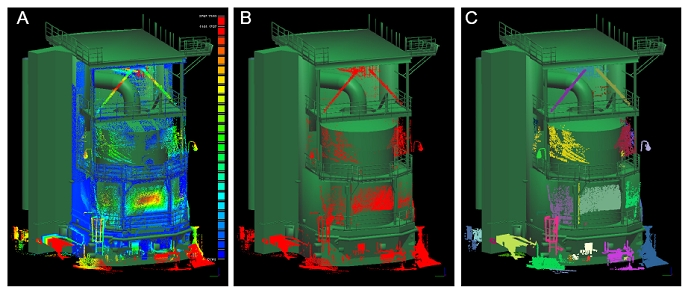
\includegraphics[width=1\textwidth]{images/Partie1_Introduction/illustration_CloudCompare.jpg}\\
\par
Depuis, CloudCompare a beaucoup �volu� et il offre d�sormais de nombreuses fonctions d'�dition (transformation rigide interactive, segmentation interactive), de recalage automatique (type ICP), de mod�lisation (calcul de maillages surfaciques type Delaunay ou Poisson), de reprojection (selon le point de vue du scanner, selon une direction principale, sur un cylindre ou un c�ne, etc.), de calcul morphologiques (rugosit�, courbure, etc.) et autres. A travers un syst�me de plugins, l'utilisateur a aussi acc�s � des fonctionalit�s et librairies externes (des algorithmes issus du monde de la recherche - reconstruction de maillage par approche de type
Poisson, filtrage des points non visibles, etc. - des p�riph�riques d'acquisition comme la Kinect de
Microsoft, ou encore des shaders �volu�s pour faciliter la visualisation des entit�s 3D - Eye Dome Lighting
 ou SSAO, etc.). \\
\par
L'originalit� de \emph{CloudCompare} tient � plusieurs aspects :
\begin{itemize}
\item les structures de donn�es utilis�es : notamment un \textquotedbl{}octree\textquotedbl{}
particulier permettant de traiter tr�s rapidement des nuages de points
volumineux (plusieurs millions de points 3D).
\item un grand nombre de choix et de m�thodes pour le calcul de distance 
entre nuages de points ou entre un nuage et un maillage triangulaire (tous bas�s sur
la notion de \textit{distance au plus proche voisin}) ;
et un calcul tr�s rapide mais moins pr�cis bas� sur une distance de \emph{Chanfrein} ;
\item la possibilit� de prendre en compte les diff�rences d'�chantillonnage entre les jeux
de donn�es compar�s ;
\item la possibilit� de filtrer le bruit de mesure a posteriori ;
\item la possibilit� de prendre en compte la visibilit� du scanner pour chaque jeu de
donn�es ;
\item la gestion de champs scalaires mutliples associ�s � un m�me nuage de points (comme des distances typiquement). Ces champs scalaires peuvent �tre affich�s par coloration dynamique des points. Ils peuvent permettre aussi de moduler l'affichage de l'entit� (par filtrage des points associ�s � certaines valeurs) ou encore de segmenter le nuage associ�. Plus g�n�ralement, ils servent d'entr�e � de nombreux alogrithmes, ils peuvent �tre compos�s ensembles, etc.
\item enfin, plusieurs types de rendus �volu�s (soit temps r�el via des shaders ou \textit{offline} via un
calcul de \textit{Portion de Ciel Visible} par exemple) permettent une forte am�lioration de la lisibilit�
des donn�es 3D � l\textquoteright{}�cran.\\
\end{itemize}
\par
Il est enfin important de noter que bien que \emph{CloudCompare} soit capable
de g�rer des maillages triangulaires, ce type d'entit� reste avant tout
pour \emph{CloudCompare} un nuage de points (les sommets du maillage) muni
d\textquoteright{}une structure particuli�re (des triangles), � c�t� de nombreuses autres
structures (octree, kd-tree, couleurs, normales, champs scalaires, photos calibr�es, etc.).
L\textquoteright{}utilisateur est donc invit� � toujours garder cette
particularit� � l\textquoteright{}esprit lorsqu\textquoteright{}il
utilise \emph{CloudCompare}, et il devra en particulier toujours faire attention
au r�le de chaque entit� 3D dans les traitements propos�s par ce logiciel.


\section{Licence\index{licence}}

Le logiciel \emph{CloudCompare} est constitu� de plusieurs
\index{composants logiciels}composants logiciels :
\begin{itemize}
\item La librairie \textbf{CClib} (algorithmes)
\item La librairie \textbf{qCC\_db} (base de donn�es)
\item Le programme \textbf{qCC} qui utilise ces librairies
\\
\end{itemize}
Installer et utiliser ces composants signifie que vous acceptez les termes
et les conditions de leurs licences respectives. La version 2.4 et les versions
ant�rieures de ces deux composants logiciels sont la propri�t� d\textquoteright{}EDF
R\&D et de TELECOM ParisTech.\\

\par
\textbf{Licence de la librairie CClib} : \\
La librairie CClib est diffus�e sous la licence GNU LGPL (GNU
Lesser General Public Licence) telle qu\textquoteright{}elle a �t�
publi�e par la FSF (Free Software Foundation) ici :
\href{http://www.gnu.org/licenses/lgpl.html}{http://www.gnu.org/licenses/lgpl.html}\\

\par
\textbf{Licence de la librairie qCC\_db} : \\
La librairie qCC\_db est diffus�e sous la licence GNU GPL (GNU General Public Licence)
telle qu\textquoteright{}elle a �t� publi�e par la FSF (Free Software Foundation) ici : \href{http://www.gnu.org/licenses/gpl.html}{http://www.gnu.org/licenses/gpl.html}\\

\par
\textbf{Licence du programme ex�cutable qCC} : \\
Le programme qCC est diffus� sous la licence GNU GPL (GNU General
Public Licence) tel qu\textquoteright{}elle a �t� publi�e par la FSF
(Free Software Foundation) ici :
\href{http://www.gnu.org/licenses/gpl.html}{http://www.gnu.org/licenses/gpl.html}\\
\\

EDF R\&D et TELECOM ParisTech accordent � l'utilisateur les droits
d'installer et d\textquoteright{}utiliser le logiciel \emph{CloudCompare}
apr�s l'avoir t�l�charg� depuis le site \href{http://www.cloudcompare.org}{http://www.cloudcompare.org}.
Le logiciel \emph{CloudCompare} est fourni en l\textquoteright{}�tat, sans
aucune garantie explicite ou implicite. Les auteurs d�clinent toute
responsabilit� pour tout dommage direct ou indirect. L\textquoteright{}utilisateur
assume tous les risques et responsabilit�s quant � la qualit� du logiciel
\emph{CloudCompare} et de son utilisation.


\section{Installation du binaire (Windows)\index{installation}}

\emph{CloudCompare} fonctionne sous les syst�mes d'exploitation Windows (XP, Vista \& Seven)
et Linux (Debian, Ubuntu, etc.) et pour des architectures 32 ou 64 bits.\\
\par
Les versions binaires de \emph{CloudCompare} pour Windows t�l�chargeables sur le site officiel
ne comportent pas de programme d'installation. Il suffit de d�compresser l'archive .zip
contenant \index{ex�cutable}l'ex�cutable et les \index{DLL (Dynamic Link Libraries)}DLLs.\\
Voici la liste minimale des fichiers que vous devez trouver apr�s d�compression
de l'archive :
\begin{itemize}
\item qCC.exe (ex�cutable principal)
\item history.txt (l'historique des modifications)
\item license.txt (la license d'utilisation)
\item CC\_DLL.dll (librairie CClib)
\item QCC\_DB\_DLL.dll (librairie qCC\_db)
\item QtCore4.dll (DLL Qt - \href{http://qt.nokia.com}{qt.nokia.com})
\item QtGui4.dll (DLL Qt - \href{http://qt.nokia.com}{qt.nokia.com})
\item QtOpenGL4.dll (DLL Qt - \href{http://qt.nokia.com}{qt.nokia.com})
\\
\end{itemize}

\par
Et de mani�re optionnelle :
\begin{itemize}
\item un certain nombre de DLLs suppl�mentaires n�cessaires � certains plugins 
(freenect.dll, etc.) ou � la prise en charge de formats de fichiers (liblas.dll, etc.)
\item un sous-r�pertoire \textit{plugins} contenant les DLLs de chaque plugin
\item un sous-r�pertoire \textit{shaders} contenant les fichiers requis par certains plugins
\item un sous-r�pertoire \textit{imageformats} contenant les librairies n�cessaires � la lecture
et l'�criture de fichiers images
\\
\end{itemize}

\par
Sous Linux, il faut imp�rativement compiler le projet pour l'utiliser (voir ci-dessous).


\section{Compilation du projet\index{compilation}}

L'int�gralit� du code de \emph{CloudCompare} est �crite en C++. Le projet utilise d�sormais le g�n�rateur de projets de compilation \emph{CMake} (\href{http://www.cmake.org/}{http://www.cmake.org}).\\
\par
Pour compiler le projet, r�f�rez vous au \emph{wiki} : \href{http://www.cloudcompare.org/doc/wiki}{http://www.cloudcompare.org/doc/wiki}\\


%---- Interface ----
\chapter{Interface}
\label{cha:Interface}

\section{Fen�tre principale}
\label{section:mainWindow}

La fen�tre principale de \emph{CloudCompare} est constitu�e des �l�ments
suivants :\\


\begin{center}
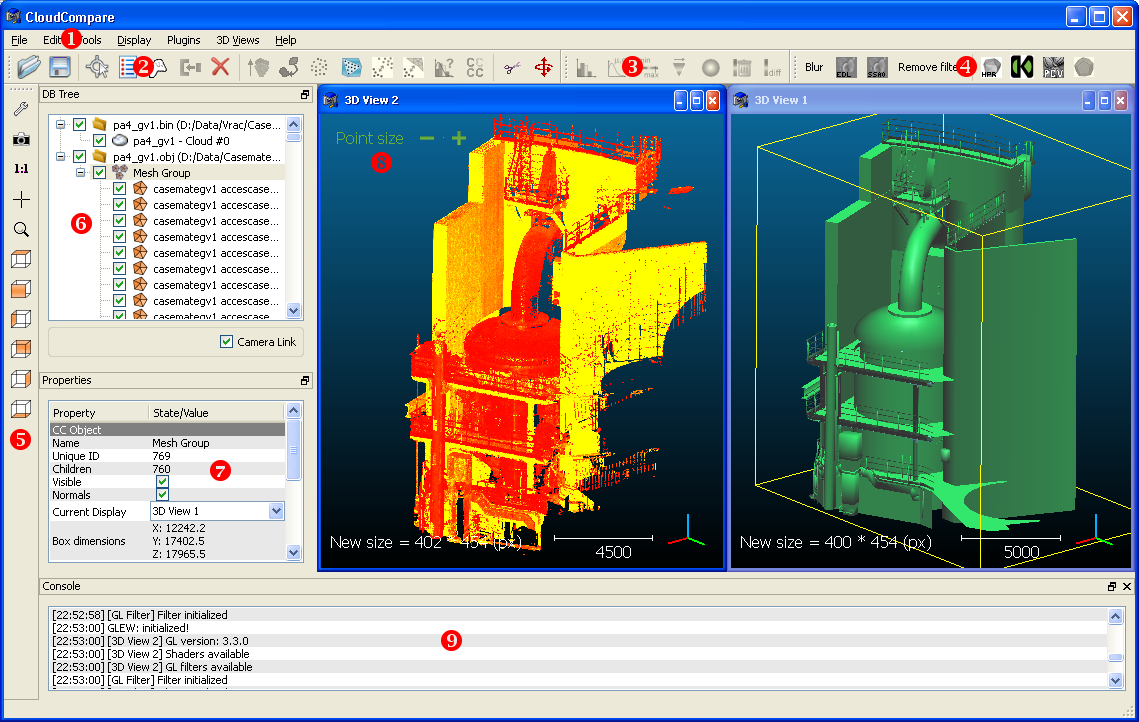
\includegraphics[width=0.9\textwidth]{images/Partie2_Interface/MainWindow}\\
\end{center}

\par
\textbf{\textcolor{red}{1}} : \index{menus, barre de}Barre de menus de l'application\\
Cette barre permet d'acc�der � la majorit� des fonctions de \emph{CloudCompare} ainsi qu'aux param�tres
de l'application et � divers outils de gestion de l'interfa�e graphique. En fonction des objets s�lectionn�s,
certains des menus ou sous-menus ne sont pas accessibles (par exemple, les menus << Edit >> et << Tools >>
restent inactifs tant qu'aucun objet n'est s�lectionn� et le sous-menu << Scalar fields >> du menu << Edit >>
ne sera accessible que si l'entit� s�lectionn�e poss�de au moins un champ scalaire).\\

\par
\textbf{\textcolor{red}{2-5}} : \index{outils, barre de}Barres d'outils\\
Les diff�rentes ic�nes de ces barres permettent d'acc�der
rapidement aux fonctions principales de \emph{CloudCompare}. Ces fonctions sont g�n�ralement aussi
accessibles via les menus situ�s au dessus (voir \textbf{\textcolor{red}{1}}) mis � part les deux
outils de modifiation interfactive des entit�s 3D (segmentation et transformation) et certains
outils de modification de l'affichage 3D (zoom, centre de rotation, points de vue pr�d�finis, etc.).
\begin{itemize}
\item la barre \textbf{\textcolor{red}{2}} (\emph{Main tools}) contient des ic�nes des fonctions de traitement
des entit�s 3D.
\item la barre \textbf{\textcolor{red}{3}} (\emph{Scalar field tools}) contient des ic�nes de fonctions de
traitement des champs scalaires.
\item la barre \textbf{\textcolor{red}{4}} (\emph{Plugins}) contient les ic�nes des plugins. La premi�re partie est
consacr�e aux plugins de type \emph{OpenGL filters} (shaders) et la seconde aux plugins standards (algorithmes). Cette
barre est remplie dynamiquement en fonction des plugins charg�s par le programme au lancement.
\item la barre \textbf{\textcolor{red}{5}} (\emph{Viewing tools}) permet de modifier les param�tres de visualisation 3D.
\\
\end{itemize}
Toutes ces barres sont d�pla�ables (par \emph{glisser-d�placer} ou \emph{drag \& drop} en anglais).
Leur visibilit� peut �tre modifi�e via le sous-menu << Display > Toolbars >>.\\

\par
\textbf{\textcolor{red}{6}} : \index{Arbre de navigation|see{navigation}}Arbre de navigation\\
Dans cette zone appara�t une repr�sentation graphique de la \emph{base de donn�es} actuellement en m�moire. Elle permet de visualiser sous forme d'arborescence l'ensemble des entit�s charg�es ou cr��es par l'application (voir section \ref{Arbre-de-navigation}). Il est notamment possible de s�lectionner une ou plusieurs entit�s en cliquant sur leur nom dans cet arbre (l'autre mani�re de s�lectionner des entit�s est de cliquer sur leur repr�sentation dans la vue 3D associ�e - voir \textbf{\textcolor{red}{8}}). Lorsque une entit� est s�lectionn�e, des informations et options sont affich�es dans la vue \textbf{\textcolor{red}{7}} (voir ci-dessous).\\

\par
\textbf{\textcolor{red}{7}} : \index{propri�t�s, fen�tre de}Fen�tre de propri�t�s\\
Si une seule entit� est s�lectionn�e, cette vue contient des informations et certaines
options d'affichage notamment (voir section \ref{Fenetre_proprietes}).\\

\par
\textbf{\textcolor{red}{8}}: \index{Vues 3D}Vues 3D\\
Ces vues permettent de visualiser en trois dimensions les entit�s g�om�triques
(nuages, maillages, etc.). \emph{CloudCompare} offre la possibilit� de cr�er plusieures vues
3D � la fois. Ces vues peuvent �tre g�r�es via le menu d�di� << 3D Views >>. Chaque entit�
peut-�tre affect�e � une vue 3D particuli�re via ses propri�t�s (voir la liste d�roulante
\emph{Current Display} des propri�t�s communes en section \ref{subsection:commonProperties}).\\

\par
\textbf{\textcolor{red}{9}} : \index{console}console\\
Cette zone contient l'historique des informations li�es � l'ex�cution de \emph{CloudCompare}
(typiquement des informations suppl�mentaires non estentielles d�livr�es par les algorithmes).
Elle peut �tre affich�e ou masqu� via la commande \emph{Console} du menu << Display >>
(raccourci clavier : F8).\\

\par
Dans la suite de cette section, nous allons d�tailler les fonctionnalit�s relatives � la manipulation et � la visualisation des diff�rentes entit�s de la base de donn�es de \emph{CloudCompare}. L'utilisateur pourra se r�f�rer directement au chapitre suivant (Chapitre~\ref{cha:Fonctions}) pour obtenir des informations d�taill�es sur les fonctions et algorithmes applicables � ces entit�s.\\



\section{Base de donn�es}

\subsection{Arbre de navigation\label{Arbre-de-navigation}\index{navigation, fen�tre de}}

\begin{center}
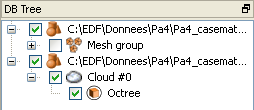
\includegraphics[width=0.4\textwidth]{images/Partie2_Interface/DBTree}
\end{center}

\par
Comme nous l'avons vu pr�c�demment, \emph{CloudCompare} affiche l'ensemble des entit�s disponibles
(charg�es ou cr�ees par l'application) dans l'arbre de navigation qui se trouve par d�faut dans la
partie sup�rieure gauche de la fen�tre principale.\\

\par
On peut y trouver les �l�ments suivants :\\
\begin{tabular}{>{\raggedright}m{0.05\textwidth}>{\raggedright}m{0.95\textwidth}}

\includegraphics[height=15px]{images/Partie2_Interface/hObjectSymbol}  & Un groupe d'entit�s.
Cet �l�ment peut correspondre par exemple � un fichier ouvert (auquel cas il contient toutes les entit�s
charg�es � partir de ce fichier). Il peut aussi �tre cr�� et peupl� manuellement (voir plus bas).\tabularnewline

\includegraphics[height=15px]{images/Partie2_Interface/CloudSymbol}  & Un nuage de points.\tabularnewline

\includegraphics[height=15px]{images/Partie2_Interface/MeshSymbol}  & Un maillage triangulaire simple.\tabularnewline
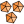
\includegraphics[height=15px]{images/Partie2_Interface/MeshGroupSymbol}  & Un ensemble de maillages triangulaires partageant
les m�mes sommets (qui sont alors contenus dans un seul nuage de points, qu'on retrouve toujours plus bas dans l'arborescence
sous le nom << vertices >>).\tabularnewline

\includegraphics[height=15px]{images/Partie2_Interface/OctreeSymbol} & Une structure de type \textit{octree}.\tabularnewline

\includegraphics[height=15px]{images/Partie2_Interface/SensorSymbol} & Un objet de type capteur laser terrestre.\tabularnewline

\includegraphics[height=15px]{images/Partie2_Interface/ImageSymbol} & Une photo non calibr�e.\tabularnewline

\includegraphics[height=15px]{images/Partie2_Interface/calibratedImageSymbol} & Une photo calibr�e.\tabularnewline

\includegraphics[height=15px]{images/Partie2_Interface/labelSymbol} & Une �tiquette 2D standard (associ�e � un ou plusieurs point).\tabularnewline

\includegraphics[height=15px]{images/Partie2_Interface/rectLabelSymbol} & Une �tiquette \textit{zone 2D} (associ�e � un point de vue).\tabularnewline

\includegraphics[height=15px]{images/Partie2_Interface/dbSymbol} & Un tableau de donn�es partag� par plusieurs entit�s (des normales par exemple).\tabularnewline

\includegraphics[height=15px]{images/Partie2_Interface/materialSymbol} & Un ensemble de mat�riaux (g�n�ralement associ� � un ou plusieurs maillages).\tabularnewline

\includegraphics[height=15px]{images/Partie2_Interface/viewportSymbol} & Un point de vue 3D (avec les param�tres de visualisation associ�s).\tabularnewline
\end{tabular}\\

\par
De mani�re classique, l'\index{arborescence|see{navigation}}arborescence peut �tre
d�velopp�e ou repli�e en cliquant respectivement sur les boutons 
\includegraphics{images/Partie2_Interface/Button+}
et 
\includegraphics{images/Partie2_Interface/Button-} situ�s � gauche des jonctions de l'arbre.\\
\par
La case � cocher situ�e � gauche du nom d'un �l�ment permet elle d'activer ou de d�sactiver la branche de l'arbre qui en part. La notion de d�sactivation est plus forte qu'un simple affichage/masquage de l'entit� (toute entit� affichable dans une vue 3D poss�de une propri�t� g�n�rique \emph{Visible} qui permet de g�rer ceci - voir plus loin). La d�sactivation d'une entit� s'applique � l'entit� elle-m�me et � toutes les entit�s qui lui sont ratach�es dans l'arboresence). Ces entit�s ne sont pas affich�es et ne sont pas non plus concern�es par certaines op�rations (comme la segmentation graphique interactive, voir section\ref{subsection:graphicalSegmentation}).\\
\par
Remarque : les groupes d'entit�s sont juste des \emph{conteneurs}. Ils n'aggr�gent pas les caract�ristiques des �l�ments qu'ils contiennent (un groupe de nuage n'est pas consid�r� comme un nuage). Typiquement, un groupe ne peut pas �tre utilis� comme entr�e pour les fonctions de \emph{CloudCompare} : il ne sert que de classeur.\\

\subsection{S�lectionner des entit�s\index{s�lectionner!des entit�s}}

Pour s�lectionner une entit�, deux possibilit�s s'offrent � l'utilisateur : cliquer avec le bouton gauche de la souris soit sur l'entr�e correspodante dans l'arbre de navigation, soit sur sa repr�sentation dans la vue 3D (ceci est vraie pour certaines entit�s seulement : nuages, maillages et �tiquettes 2D). Dans les deux cas, l'entr�e correspondante dans l'arbre de navigation appara�t surlign�e et l'entit� est entour�e d'une \index{bo�te englobante} bo�te englobante dans \index{Vue 3D}la vue 3D o� appara�t l'entit�. Lorsqu'un �l�ment est s�lectionn�,
les informations qui s'y rapportent apparaissent dans la fen�tre de propri�t�s (voir section \ref{Fenetre_proprietes}).\\
\par
Il est possible de s�lectionner plusieurs entit�s en ayant recours aux m�thodes classiques de \index{s�lection multiple|see{s�lectionner}}s�lection multiple :
\begin{itemize}
\item s�lection des entit�s une par une en cliquant dessus (dans l'arbre de navigation ou dans une vue 3D) tout en maintenant la touche CTRL enfonc�e. Pour d�-s�lectionner un objet tout en conservant ceux qui ont d�j� �t� s�lectionn�s, il faut cliquer une nouvelle fois dessus tout en maintenant la touche CTRL enfonc�e.
\item s�lection d'une s�rie continue d'entit�s avec la touche MAJ (dans l'arbre de navigation uniquement) : s�lectionner la premi�re entit�, presser et maintenir la touche MAJ enfonc�e tout en s�lectionnant la derni�re entit�.
\item toujours dans l'arbre de navigation, on peut enfin survoler les objets � s�lectionner en maintenant le bouton gauche de la souris enfonc�.\\
\end{itemize}

\par
La plupart des fonctions de \emph{CloudCompare} ne s'appliquent qu'aux entit�s s�lectionn�es.
Les entr�es des menus correspondantes ne sont d'ailleurs actives que lorsque l'utilisateur a s�lectionn�
le type et le nombre d'entit�s appropri�s (par exemple, deux nuages ou un nuage et un maillage pour le
calcul de distances).\\

\subsection{Int�ractions avanc�es avec l'arbre de navigation}

Il est possible de d�placer les entit�s dans l'arbre de navigation par \emph{drag \& drop} (pour les regrouper dans un m�me << groupe >> par exemple). Les << groupes >> sont cr�es automatiquement lors du chargement depuis un fichier (auquel cas le groupe prend le nom du fichier) mais ils peuvent aussi �tre cr��s par clic sur un �l�ment de l'arbre de navigation (ou dans une partie vide pour cr�er le groupe � la racine).\\

Attention : d�placer ainsi les entit�s change leurs relations hi�rarchiques (ce qui peut avoir des cons�quences importantes lors de certaines actions, comme la sauvegarde ou la suppression de l'entit� parente). De plus les entit�s ne peuvent pas �tre d�plac�es n'importe o� pour maintenir la coh�rence interne de la base de donn�es.\\

\begin{center}
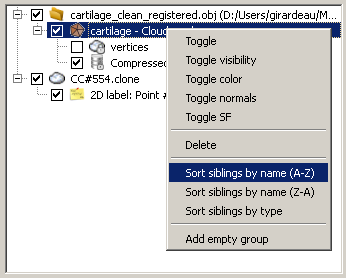
\includegraphics[width=0.4\textwidth]{images/Partie2_Interface/contextMenuRightClick}
\end{center}

\par
Un clic droit sur un �l�ment de l'arbre de navigation fait apparaitre un menu contextuel (dont le contenu d�pend de l'entit�). On retrouve toujours les entr�es suivantes :
\begin{itemize}
\item \emph{Toggle} - inverse l'�tat d'activation de l'entit�
\item \emph{Delete} - supprime l'entit�
\item \emph{Add empty group} - rajoute un << groupe >> (sous l'entit�)\\
\end{itemize}

\par
Si l'entit� est affichable en 3D (nuage, maillage, �tiquette 2D, etc.), des options suppl�mentaires permettent d'inverser l'�tat de \emph{visibilit�} de l'entit� elle-m�me et de ses composantes �ventuelles (couleurs, normales, champ scalaire, etc.).\\
\par
Enfin, si l'entit� poss�de plusieurs sous-entit�s dans l'arbre, des options permettant la r�organisation
de ces sous-entit�s peuvent apparaitre (tri automatique par nom, ou tri par type).\\

\subsection{Entit�s particuli�res}

\subsubsection{L'octree}\index{octree}

L'octree est une structure destin�e � acc�l�rer les traitements sur des donn�es spatiales.
Il s'agit d'un d�coupage r�cursif et hi�rarchique de l'espace (en \emph{cubes}).
\emph{CloudCompare} associe les nuages de points avec une telle structure dans de tr�s nombreux cas pour acc�lerer ses traitements. C'est un type d'octree particulier qui est particuli�rement rapide � construire, et optimis� pour la recherche de plus proches voisins (\textit{ce n'est par contre pas un octree efficace pour l'affichage de type L.O.D. - level of detail - typiquement}).\\
\par
D'un point de vue g�n�ral, l'octree est d�fini par \emph{niveaux de subdivison} :
\begin{itemize}
\item Le premier niveau (niveau 0) est le plus petit cube englobant enti�rement
le nuage de points (une version \textit{cubifi�e} de la boite englobante).
\item Au niveau $N+1$, l'octree est construit en subdivisant chacun des cubes du
niveau $N$ en 8 sous-cubes de m�me taille (en pratique on ne se souvient que des
sous-cubes contenant au moins un point).\\
\end{itemize}
\par
Il n'est pas inint�ressant pour l'utilisateur de comprendre le principe de cette structure, puisqu'elle occupe une place centrale dans \emph{CloudCompare}.\\
\par
Plus le niveau d'octree est �lev� :
\begin{itemize}
\item plus le nombre de cubes � traiter est �lev� : potentiellement $8^{N}=2^{3N}$
cubes au niveau $N$. Pour un ordre d'id�es, et bien que cela soit tr�s peu probable, on peut donc
avoir jusqu'� $2^{21}=2~097~152$ de cubes au niveau 7 de l'octree. Au niveau 10, on a
$2^{30}$ cubes, soit un peu plus d'un milliard ! (l� encore, cela est extr�mement peu
probable ... d'autant plus qu'il faudrait au moins autant de points). En pratique, beaucoup
de cubes sont vides et ne sont donc pas conserv�s en m�moire, d'o� une structure
g�n�ralement beaucoup plus compacte. Enfin, \emph{CloudCompare} utilise un codage sp�cial
de l'octree qui fait que sa taille est toujours �gale au nombre de points du
nuage, et ne d�pend donc pas de la r�partition spatiale de celui-ci. \textbf{C'est aussi pour cette
raison que le niveau maximal d'un octree est fix� � 10 dans la version actuelle de \emph{CloudCompare}} (ce qui permet de coder la position de chaque point et pour tous les niveaux de l'octree sur 3*10 = 30 bits, ce qui tient dans une valeur enti�re de 4 octets = 32 bits, soit un codage par point pas trop gourmand en m�moire).
\item plus les cubes sont petits : si $a_{N}$ est la taille d'une ar�te
du cube au niveau $N$ (donc $a_{0}$ est la taille du cube initial), $a_{N}=\frac{a_{0}}{2^{N}}$.
En effet, par construction, on divise par deux la taille des cubes selon chaque dimension lorsque l'on descend d'un niveau. Par exemple, les cellules de l'octree au niveau 5 d'un octree sont 32 fois plus petites que la cellule initiale englobant tout le nuage (au niveau 0).
\item plus le nombre de points par cube est faible : intuitivement, les cubes �tant plus petits, ils contiennent (statistiquement) moins de points.
\item plus l'enveloppe de l'octree (la surface globale qui serait form�e par l'ensemble des surfaces externes des cubes) est proche du nuage de points originale.\\
\end{itemize}

\begin{figure}[!htb]
\begin{center}
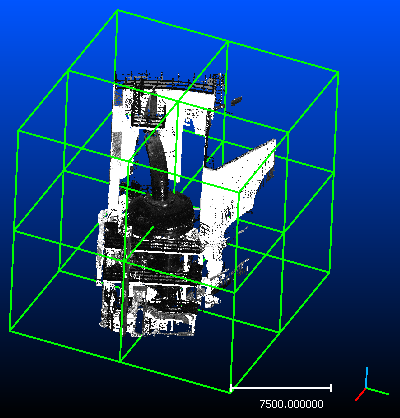
\includegraphics[width=0.3\textwidth]{images/Partie2_Interface/OctreeLevel1}\hfill{}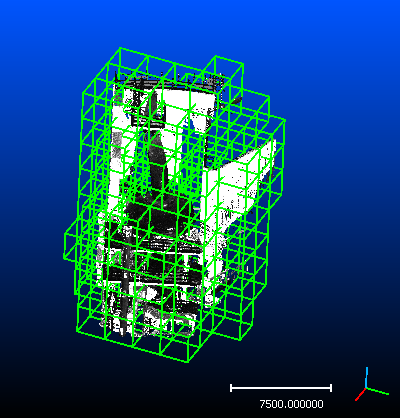
\includegraphics[width=0.3\textwidth]{images/Partie2_Interface/OctreeLevel3}\hfill{}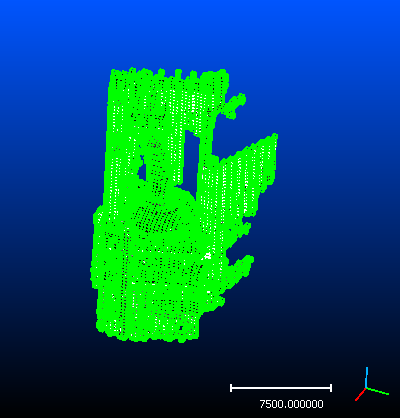
\includegraphics[width=0.3\textwidth]{images/Partie2_Interface/OctreeLevel6}\\
\caption{\label{fig:octreeLevel}Cellules � diff�rents niveaux d'octree : niveau
1 (gauche), 3 (milieu) et 6 (droite).}
\end{center}
\end{figure}

Les 3 captures d'�cran de la figure~\ref{fig:octreeLevel} donnent un aper�u de la r�partition
et de la taille des cellules d'octree � differents niveaux de subdivision.\\

Beaucoup de traitements sur les nuages de points ont recours � un octree. Lorsque cela est possible, le niveau d'octree optimal pour les calculs � effectuer est d�termin� de mani�re automatique par \emph{CloudCompare}. Toutefois, certains algorithmes peuvent demander � l'utilisateur de sp�cifier un niveau spcifique � utiliser. Dans ces situations, il s'agit g�n�ralement pour l'utilisateur de trouver un niveau qui aboutisse au meilleur compromis entre le nombre de cubes � traiter (qu'on ne veut g�n�ralement pas trop grand, donc une valeur de niveau pas trop �lev�e) et le nombre moyen de points par cube (qu'on ne veut g�n�ralement le plus petit possible, donc une valeur de niveau ... pas trop faible). Trouver le bon niveau peut parfois n�cessiter une certaine exp�rience.\\


\subsubsection{Etiquettes 2D et annotation graphique\index{etiquettes}\label{etiquettes_2D}}

CloudCompare permet d'annoter\index{annotation} un ensemble d'entit�s 3D via des �tiquettes (\textit{2D labels}) de diff�rents types.\\
\par
Remarque : ces �tiquettes peuvent �tre sauv�es via le format binaire propre � CloudCompare (BIN).\\

\par
\textbf{Etiquette standard}\label{subsection:standardLabel}\\

\begin{figure}[!htb]
\begin{centering}
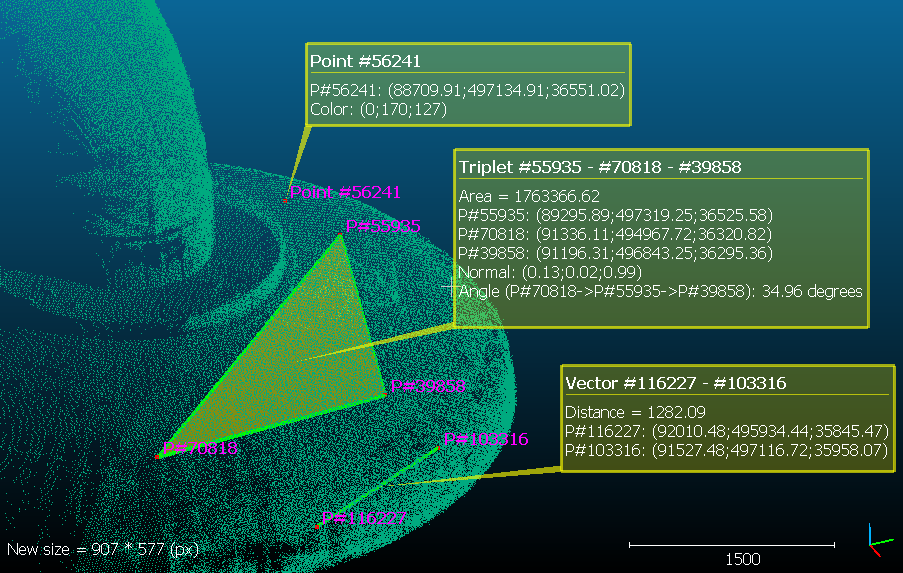
\includegraphics[width=0.8\textwidth]{images/Partie2_Interface/standardLabels}
\caption{\label{fig:standardLabels}Etiquettes standards}
\end{centering}
\end{figure}

Le premier type, \emph{2D label}, correspond aux �tiquettes (mobiles) rattach�es � un ou plusieurs points :
\begin{itemize}
\item un point : l'�tiquette continent les coordonn�es du point, son indice dans le nuage et les valeurs de ses diff�rents champs (couleur, normale, champ scalaire affich�)
\item deux points (segment) : l'�tiquette contient les coordonn�es de chaque point et leur indice respectif dans le(s) nuage(s) ainsi que la distance entre les deux points
\item trois points (triangle) : l'�tiquette contient les coordonn�es de chaque point et leur indice respectif dans le(s) nuage(s), l'aire du triangle ainsi d�fini, la normale au triangle, et enfin l'angle au niveau du premier point (\textsl{l'ordre de s�lection des points est donc important})\\
\end{itemize}

\par
La repr�sentation graphique des �tiquettes standards peut �tre modul�e en fonction des besoins : leur titre peut �tre affich� en 3D � c�t� du ou des points auxquelles elles sont associ�es, tandis que leur repr�sentation 2D peut �tre soit affich�e totalement, soit affich�e de mani�re condens�e soit encore cach�e. La repr�sentation 2D a de plus une transparence r�glable (via les param�tres d'affichage g�n�raux de CloudCompare - voir section\ref{subsection:displaySettings}). A l'instar des nuages de points ou les maillages, les �tiquettes standards peuvent �tre s�lectionn�es � l'�cran (s�lection multiple ou individuelle).\\
\par
Les �tiquettes rattach�es � un unique point peuvent �tre cr��es tr�s facilement (\textit{� la vol�e}) par un simple clic sur le point en maintenant la touche SHIFT enfonc�e. Autrement, tous les autres type d'�tiquettes peuvent �tre cr�es avec l'outil 'Point Picking' (Cf. section \ref{subsection:pointPicking}).\\

\par
\textbf{Etiquette \emph{zone 2D}}\label{subsection:zoneLabel}\\

\begin{figure}[!htb]
\begin{centering}
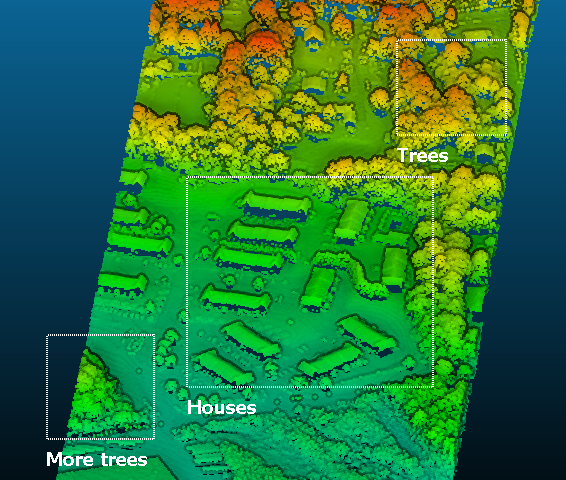
\includegraphics[width=0.5\textwidth]{images/Partie2_Interface/zoneLabels}
\caption{\label{fig:standardLabels}Etiquettes \emph{zone 2D}}
\end{centering}
\end{figure}

\par
Le second type d'�tiquette, \emph{2D area label}, correspond aux �tiquettes fixes rattach�es � un point de vue. Ce sont des zones rectangulaires (d�finies par l'utilisateur � l'�cran) associ�es � un commentaire textuel.\\

\par
Etant donn� que ce qui appara�t dans la zone d�limit�e par l'�tiquette d�pend du point de vue (orientation de la cam�ra, etc.), l'�tiquette n'apparait que lorsque la cam�ra est dans la m�me position (et avec les m�mes param�tres) que lorsqu'elle a �t� cr��e (seuls certains param�tres peuvent �tre compens�s automatiquement, comme le zoom ou le panning en mode orthographique). Pour simplifier la t�che de l'utilisateur, les �tiquettes \emph{zone 2D} sont donc capables de r�tablir ces param�tres dans la vue 3D associ�e (un bouton \emph{Apply} se trouve dans les propri�t�s de l'�tiquette - voir section \ref{subsection:zoneLabelProp}).


\section{Affichage des entit�s}

\subsection{Vues 3D\label{Contexte-graphique}\index{Vue 3D}}

\subsubsection{Pr�sentation}

Les vues 3D (voir figure~\ref{fig:Context3D}) sont les sous-fen�tres dans lesquelles sont affich�es les entit�s.
Elles poss�dent un fond (qui peut-�tre un d�grad� de couleur ou une couleur unique - voir les param�tres d'affichage
g�n�raux en section \ref{subsection:displaySettings}), par dessus lequel sont affich�es les entit�s 3D (nuages, maillages,
etc.) et encore par dessus, des �l�ments d'interface ou des entit�s 2D (�tiquettes, �chelle de couleur, etc.).\\

Voici les �l�ments standards qui composent une vue 3D :
\begin{itemize}
\item \textbf{\textcolor{red}{1}} : les entit�s 3D, �ventuellement encadr�es par leur boite englobante\footnote{Aussi appell�e \textit{bounding-box}. Il s'agit du plus petit parall�l�pip�de rectangle align� avec les axes principaux (X,Y,Z) et qui contienne l'int�gralit� des entit�s s�lectionn�es} si elles sont s�lectionn�es).
\item \textbf{\textcolor{red}{2}} : l'\index{echelle@�chelle!de distances}�chelle fournit une r�f�rence pour
l'estimation des dimensions. Sa longueur est exprim�e dans l'unit� \textit{impliticte} courante (i.e. l'unit� implicite des coordonn�es de la ou des entit�s affich�es, telles qu'elles ont �t� charg�es depuis leur fichier d'origine - \emph{CloudCompare} n'utilise pas d'unit� explicite).
\item \textbf{\textcolor{red}{3}} : le \index{tri�dre d'orientation}tri�dre d'orientation repr�sente l'orientation
courante des trois axes principaux : X (rouge), Y (vert) et Z (bleu).
\item \textbf{\textcolor{red}{4}} : nom du \index{champ scalaire}champ scalaire actif et sa
\index{rampe de couleurs}\index{echelle@�chelle!de couleurs|see{rampe de couleurs}}rampe de couleurs associ�e.
\item \textbf{\textcolor{red}{5}} : informations temporaires concernant l'affichage ou l'action en cours. Il peut s'agir de la dimension courante de la vue 3D (en pixels - apr�s un redimensionnement de la fen�tre), du type de projection utilis�, etc.
\item \textbf{\textcolor{red}{6}} : \index{�tiquette 2D}�tiquette 2D standard (ici associ�e � un point 3D d'un nuage). Ces �tiquettes s'affichent toujours par dessus les objets 3D (leur transparence est r�glable). Pour plus d'information, Cf. section\ref{etiquettes_2D}.
\item \textbf{\textcolor{red}{7}} : \index{Annotation}�tiquette \textit{zone 2D}. Ces �tiquettes particuli�res
permettent d'annoter une zone pr�cise de l'�cran et sont donc li�es � un point de vue (qu'elles sont capable de r�tablir sur demande) et non � une entit�.\\
\end{itemize}

\begin{figure}[!htb]
\begin{centering}
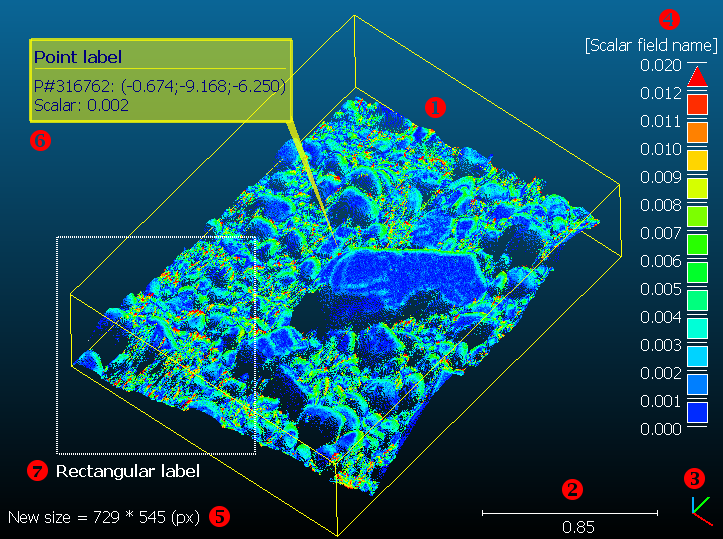
\includegraphics[width=0.8\textwidth]{images/Partie2_Interface/View3D}
\caption{\label{fig:Context3D}El�ments standards d'une vue 3D}
\end{centering}
\end{figure}

Seuls l'�chelle et le tri�dre d'orientation sont visibles en permanence.
Les autres informations d�pendent de l'�tat courant de l'application.\\

\subsubsection{Interagir avec une vue 3D\label{subsection:Interactivit�}}

Vous pouvez int�ragir avec une vue 3D en utilisant la\index{souris} souris (figure \ref{fig:mouseButtons}) :\\

\begin{figure}[!htb]
\begin{centering}
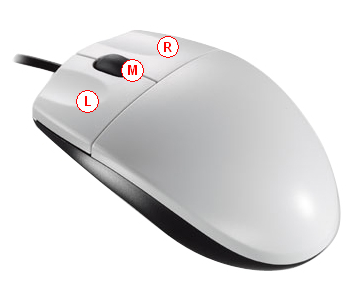
\includegraphics[width=0.4\textwidth]{images/Partie2_Interface/Souris}
\caption{\label{fig:mouseButtons}Commandes via la souris (L : [SELECTION/ROTATION], M : [ZOOM], R : [PAN])}
\end{centering}
\end{figure}


\begin{itemize}
\item \textbf{\textcolor{red}{L}} - clic gauche court : [SELECTION] cliquez sur un objet
dans la vue 3D pour le s�lectionner.
\item \textbf{\textcolor{red}{L}} - clic gauche maintenu : [ROTATION] maintenez le bouton gauche
de la souris enfonc� et d�placez la souris pour effectuer une rotation
du point de vue autour du \textit{pivot} courant (cf. sections
\ref{subsection:centeredPerspective} et \ref{subsection:viewerPerspective} ou encore
les param�tres cam�ras en section \ref{subsection:cameraSettings} ou enfin l'outil de
picking du centre de rotation en section \ref{Options-affichage}).
\item \textbf{\textcolor{red}{M}} - roulement : [ZOOM] faites rouler la molette
vers l'avant (ou vers \og le haut \fg{}) pour effectuer un \index{zoom}zoom positif
dans la vue 3D et inversement, faites rouler la molette vers l'arri�re (ou \og le
bas \fg{}) pour effectuer un zoom n�gatif.
\item \textbf{\textcolor{red}{R}} - clic droit court : sur les �tiquettes 2D, un clic droit court
permet de la condenser ou inversement de r�tablir son extension maximale.
\item \textbf{\textcolor{red}{R}} - clic droit maintenu : [PANNING] maintenez le bouton droit
de la souris enfonc� et d�placez la souris pour effectuer une translation du point de vue
dans le plan �cran.\\
\end{itemize}

Par d�faut, la visualisation se fait selon une projection orthographique (sans perspective) et le
centre de rotation est positionn� sur le centre de la boite englobant toutes les entit�s affich�es
dans la vue 3D. Lors du changement de point de vue (rotation, translation), les gros
nuages de points ou les gros maillages sont temporairement sous �chantillonn�s de mani�re � permettre
le rendu interactif des mouvements (ce comportement est param�trable - voir section\ref{subsection:displaySettings}).\\

\subsubsection{Utiliser plusieurs vues 3D\label{Environnement-multi-contextes}}

Dans CloudCompare, un nombre quelconque de vues 3D peut �tre cr��, et chaque entit� peut �tre
assign�e s�par�mment � une vue 3D particuli�re.\\

Pour cr�er une nouvelle vue 3D, cliquez sur la commande
\emph{New} dans le menu << 3D views >>, ou utilisez le raccourci clavier
CTRL+F3. Une nouvelle fen�tre appara�t alors (par d�faut elle sera maximis�e).\\

\par
Pour partager l'espace d'affichage entre les diff�rentes vues 3D,
diff�rents choix s'offrent � l'utilisateur :
\begin{itemize}
\item \emph{Tile} (partitionnement) : chaque fen�tre occupe une portion
"�quivalente de l'espace disponible, les fen�tres ne se chevauchent pas.
\item \emph{Cascade}  : chaque fen�tre occupe la m�me portion d'espace
pr�d�finie, elles sont d�cal�es de mani�re r�guli�re en se chevauchant.
\item redimensionnement manuel : de mani�re classique chaque vue 3D
peut-�tre d�plac�e et redimensionn�e, en s'aidant notamment des boutons 
\includegraphics{images/Partie2_Interface/ReduceContext}(minimiser
la vue) et 
\includegraphics{images/Partie2_Interface/MinimizeContext}(r�duire
la vue) disponibles en haut � droite de chaque fen�tre.\\
\end{itemize}

\par
Il est aussi possible de naviguer entre les diff�rentes vues via les commandes
\emph{Next} et \emph{Previous} du menu << 3D views >>, ou en acc�dant directement
� la vue d�sir�e en cliquant sur son nom dans ce m�me menu.\\

\par
Pour fermer une vue 3D, utilisez l'entr�e \emph{Close} du menu << 3D views >> (apr�s
avoir activ� cette fen�tre en cliquant dessus) ou plus simplement utilisez le bouton 
\includegraphics{images/Partie2_Interface/CloseContext} de la fen�tre.\\

\par
Enfin, pour changer la \index{afficher!des objets}vue 3D dans laquelle une entit�
appara�t, s�lectionnez cette entit� puis modifiez la valeur courante de la liste
d�roulante \emph{Current Display} dans la fen�tre de propri�t�s.

\begin{center}
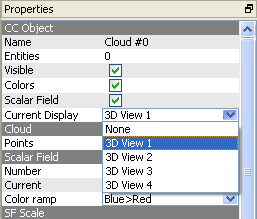
\includegraphics[width=0.4\textwidth]{images/Partie2_Interface/ChangeContext}
\par
\end{center}

Remarque : il est possible de n'afficher une entit� dans aucune vue 3D en choisissant
\emph{None} comme \textit{contexte} de destination.\\


\subsubsection{Camera link\label{subsection:cameraLink}}

Les vues 3D sont ind�pendantes les unes des autres, et les changements de point de vue dans une vue 3D particuli�re n'ont a priori aucune r�percussion sur les autres vues 3D. Toutefois, il est possible de synchroniser les mouvements de cam�ra pour qu'ils soient appliqu�s � toutes les \index{Vues 3D} vues 3D en m�me temps. Pour ce faire il suffit de cocher l'option
\emph{Camera link} situ�e juste sous l'arbre de navigation.

\begin{center}
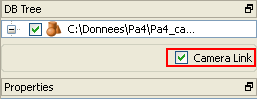
\includegraphics[width=0.4\textwidth]{images/Partie2_Interface/CameraLink}\\

\par\end{center}


\subsection{Options d'affichage\label{Options-affichage}}

\subsubsection{Barre d'outils \textit{Viewing Tools}}

Un certain nombre d'ic�nes et d'outils permettent � l'utilisateur de contr�ler l'affichage courant.
La majeure partie d'entre eux sont accessibles via la \index{outils, barre de}barre d'outils \emph{Viewing tools} :
\begin{center}
\begin{tabular}{>{\centering}m{0.05\textwidth}>{\raggedright}m{0.95\textwidth}}
\multicolumn{2}{c}{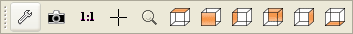
\includegraphics[height=21px]{images/Partie2_Interface/ViewToolBar}}\tabularnewline

\includegraphics[height=15px]{images/Partie2_Interface/cc_settings} & Changer les param�tres \index{eclairage@�clairage}d'affichage g�n�raux (couleurs, mat�riaux, taille de la police, pr�cision num�rique des valeurs affich�es, etc. - voir section\ref{subsection:displaySettings}).\tabularnewline

\includegraphics[height=15px]{images/Partie2_Interface/Camera} & Changer les param�tres de cam�ra de la fen�tre 3D courante (orientation et centre de rotation, etc. - voir section\ref{subsection:cameraSettings}).\tabularnewline

\includegraphics[height=15px]{images/Partie2_Interface/ZoomGlobal} & \index{zoom}Zoomer et recentrer la \index{point de vue}cam�ra pour rendre visibles toutes les entit�s affich�es dans la vue 3D courante.\tabularnewline
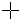
\includegraphics[height=15px]{images/Partie2_Interface/cc_pickCenter} & S�lection du centre de rotation par picking d'un point � l'�cran.\tabularnewline

\includegraphics[height=15px]{images/Partie2_Interface/ZoomCenter} & Zoomer et recentrer la cam�ra sur la ou les entit�s s�lectionn�es. Aucun effet si aucun objet n'est s�lectionn�.\tabularnewline

\includegraphics[height=15px]{images/Partie2_Interface/ChangeView} & Les 6 derniers boutons permettent de basculer entre diff�rents points de vue pr�d�finis (dans l'ordre o� les boutons apparaissent : haut, avant, gauche,
arri�re, droit, bas). Ces points de vue sont d�finis par rapport au \index{tri�dre d'orientation}tri�dre d'orientation. \tabularnewline
\end{tabular}\\
\end{center}

\subsubsection{Menu \textit{Display}}

D'autres fonctionnalit�s relatives � l'affichage sont accessibles via le menu \emph{Display} :
\begin{itemize}
\item \emph{Full screen} : basculer la fen�tre principale entre l'affichage standard et l'affichage \index{plein �cran}plein
�cran (raccourci clavier: F11).
\item \emph{Refresh} : forcer l'actualisation de l'affichage (raccourci clavier : F5).
\item \emph{Test frame rate} : lancer un test d'estimation du \index{rafra�chissement, taux de}taux de rafra�chissement
(exprim� en 'f.p.s' = \textit{frame per second} ou images par seconde en fran�ais) pour la vue 3D courante. En th�orie, plus il y a de triangles ou de points � afficher, plus le taux de rafra�chissement devrait �tre faible. Il est admis qu'en de�� d'une vingtaine d'images par seconde, l'humain per�oit l'affichage comme �tant saccad� (au del� de 24 f.p.s, l'affichage est per�u comme �tant fluide).
\item \emph{Toggle centered perspective} : basculer entre la projection par d�faut (parall�le orthographique) et la projection perspective avec le centre de rotation de la cam�ra plac� par d�faut sur le centre de la boite englobant toutes les entit�s affich�es (raccourci clavier : F3).
\item \emph{Toggle viewer based perspective} : basculer entre la projection par d�faut (parall�le orthographique) et la projection perspective avec le centre de rotation de la cam�ra plac� par d�faut en son centre optique (l'oeil virtuel de l'utilisateur) (raccourci clavier : F4).
\item \emph{Light > Toggle sun light} : activer ou \index{eclairage@�clairage}d�sactiver
la lumi�re globale (raccourci clavier : F6).
\item \emph{Light > Toggle custom light }: activer ou d�sactiver
la lumi�re personnalis�e (raccourci clavier : F7). Cette source de lumi�re peut �tre d�pla��e en maintenant la touche CTRL
enfonc�e tout en faisant un \emph{pan} avec la souris � l'�cran - voir section\ref{subsection:Interactivit�}).\\
\end{itemize}

\par
Remarque : les effets d'ombrage permis par les normales d'un nuage ou d'un maillage ne sont visibles que si au moins une source lumineuse est active.\\

\subsubsection{Taille des points 3D\label{pointSizeModification}}

La taille des points affich�s dans une vue 3D est modifiable via des \textit{interacteurs} qui apparaissent
directement en surimpression de la vue lorsque la souris survole son coin haut-gauche.

\begin{center}
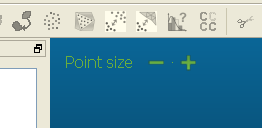
\includegraphics[width=0.3\textwidth]{images/Partie2_Interface/PointSizeDlg}
\par\end{center}

Pour modifier la \index{taille des points}taille d'affichage des points, il suffit de cliquer sur '-' ou '+'. Un point de r�f�rence � la taille courante appara�t entre les deux interacteurs.\\



\section{Fen�tre de propri�t�s}\index{propri�t�s, fen�tre de}\label{Fenetre_proprietes}

La fen�tre de propri�t�s contient toutes les informations sur l'entit� s�lectionn�e, ainsi que des options modifiables par l'utilisateur (visiblit� de certains composants, etc.).

\subsection{Propri�t�s communes des entit�s affichables}\label{subsection:commonProperties}

Certains champs sont communs � (presque) toutes les entit�s affichables. On les retrouve dans la section \emph{CC Object} :
\begin{center}
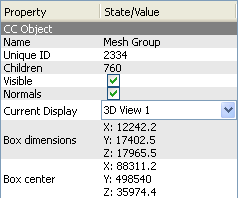
\includegraphics[width=0.4\textwidth]{images/Partie2_Interface/CommonProperties}
\par\end{center}
\begin{itemize}
\item \emph{Name} : \index{renommer}nom de l'entit�. Il peut �tre modifi� en cliquant sur l'entr�e correspondant � l'entit� dans l'arbre de navigation (voir \ref{Arbre-de-navigation}) ou encore en utilisant le raccourci clavier F2.
\item \emph{Unique ID} : toutes les entit�s CloudCompare sont repr�sent�es en interne par un identifiant unique.
\item \emph{Children} : le nombre de sous-�l�ments (ou \textit{enfants}) rattach�s � cette entit�. Dans la capture ci-dessus par exemple, l'objet s�lectionn� est un groupe de maillages regroupant 758 sous-maillages, un nuage de points et un tableau de normales compress�es, soit 760 sous-entit�s au total).
\item \emph{Visible} : sp�cifie si l'entit� doit �tre affich�e dans la vue 3D associ�e ou non. La propri�t� 'Visible' n'est pas h�r�ditaire (contrairement � l'�tat d'activation de l'entit�, qui correspond � la case � cocher pr�sente au niveau de l'arbre de navigation et qui concerne toutes les entit�s pr�sentes dans le reste de la branche). Si l'entit� est s�lectionn�e, la boite englobante reste visible m�me si la propri�t� \emph{Visible} est d�sactiv�e.
\item \emph{Colors} (optionnelle) : si l'entit� s�lectionn�e poss�de des couleurs, une case � cocher \emph{Colors} apparait ici. Elle permet de sp�cifier si ces couleurs doivent �tre utilis�es lors de l'affichage de l'entit� ou non. Remarque : la propri�t� \emph{Scalar field} (voir ci-dessous) est toujours prioritaire par rapport � \emph{Colors}.
\item \emph{Normals} (optionnelle) : si l'entit� s�lectionn�e poss�de des normales, une case � cocher \emph{Normals}  apparait ici. Elle permet de sp�cifier si ces normales doivent �tre utilis�es lors de l'affichage de l'entit� ou non. Les normales\index{normales}\index{eclairage@�clairage} permettent d'obtenir un rendu visuel semi-r�aliste des objets en faisant varier la teinte des points ou facettes associ�ess en fonction de la position de l'�clairage. Si les normales sont d�sactiv�es, la surface de l'objet est affich�e dans une couleur uniforme (effet \og silhouette \fg{}, avec une perte de la perception des profondeurs). \textit{Le plugin \emph{qEDL} (voir section\ref{qEDL}) est une excellente alternative aux normales. Il simule en temps r�el un �clairage encore plus r�aliste, sans information autre que la position des points ou des objets.}
\item \emph{Scalar field} (optionnelle) : si l'entit� s�lectionn�e poss�de un ou plusieurs champs scalaires, une case � cocher \emph{Scalar field}  apparait ici. Elle permet de sp�cifier si le champ scalaire couramment affich� (voir la liste d�roulante \emph{Current} dans la section \emph{Scalar field} des proprit�s) doit �tre utilis� lors de l'affichage de l'entit� ou non. Si un champ scalaire courant est d�fini dans la liste d�roulante \emph{Current}, alors ce champ scalaire sera toujours affich� en priorit� par rapport aux �ventuelles couleurs de l'entit�.
\item \emph{Current display} : cette liste d�roulante permet de choisir la vue 3D dans laquelle l'objet sera affich�
(cf. section \ref{Environnement-multi-contextes}).
\item \emph{Box dimensions} : les dimensions de la boite englobante de l'entit�.
\item \emph{Box center} : le centre de la boite englobante de l'entit�.\\
\end{itemize}
\par


\subsection{Propri�t�s propres aux nuages de points}\label{subsection:pointCloudProperties}

La section \emph{Cloud} est r�serv�e aux nuages de points. Elle contient les champs suivants :
\begin{itemize}
\item \emph{Points} : le nombre de points du nuage.
\item \emph{Global shift}\index{centrage automatique au chargement} : la translation qui a �t� �ventuellement appliqu�e au chargement du nuage par CloudCompare (g�n�ralement pour rammener ses coordonn�es � des valeurs compatibles avec un stockage en flottant sur 32 bits). C'est typiquement le cas des nuages exprim�s dans des syst�mes de coordonn�es � l'�chelle d'un pays (UTM, etc.), avec des valeurs d�passant les millions. Dans ce cas, CloudCompare propose � l'utilisateur de recentrer automatiquement l'entit�. Cette translation est conserv�e tout au long de la vie de l'entit� puis elle sera �ventuellement r�-appliqu�e aux points lors la sauvegarde de l'entit� (si le format le permet).
\\
\end{itemize}

\begin{center}
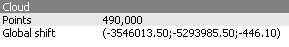
\includegraphics[width=0.5\textwidth]{images/Partie2_Interface/PointCloudProperties}
\end{center}

\subsection{Propri�t�s propres aux maillages ou groupes de maillages}\label{propMaillages}

\begin{center}
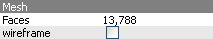
\includegraphics[width=0.4\textwidth]{images/Partie2_Interface/MeshProperties}\\
\end{center}

\index{maillage}
Les entit�s maillages ou groups de maillages deux types d'entit�s partagent les m�mes propri�t�s :
\begin{itemize}
\item \emph{Faces} : le nombre de facettes composant le maillage. Dans le cas d'un groupe de maillages, ce nombre correspond au nombre total de facettes de tous les sous-maillages rattach�s � ce groupe.
\item \emph{Wireframe} : \index{fil de fer, rendu}\index{WireFrame|see{fil de fer}}permet
d'activer le rendu en \og fil de fer \fg{} du maillage (seules les arr�tes des triangles sont affich�es et non l'int�rieur - voir figure \ref{fig:MeshWireframeRendering}).\\
\end{itemize}

\begin{figure}[!htb]
\begin{center}
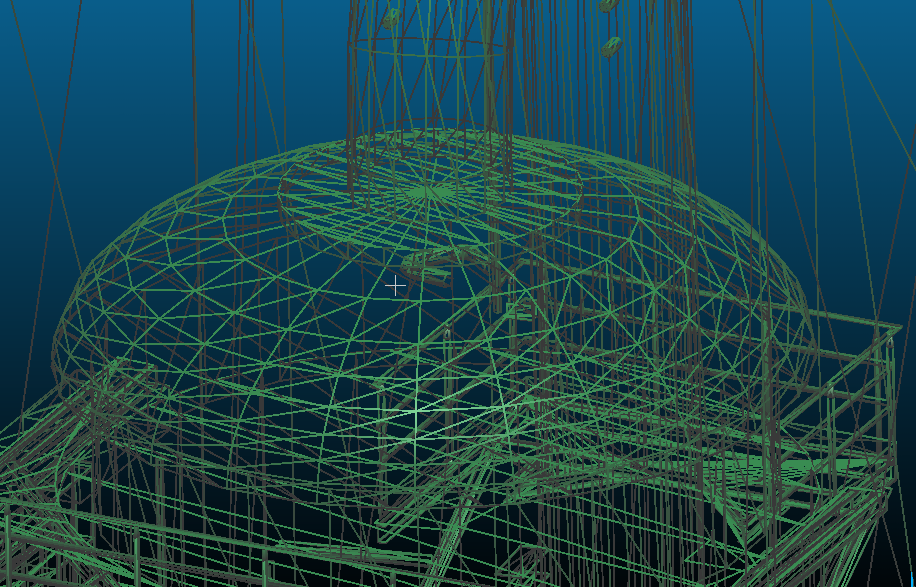
\includegraphics[width=0.6\textwidth]{images/Partie2_Interface/MeshWireframeRendering.png}
\caption{\label{fig:MeshWireframeRendering}Exemple de rendu en \textit{fil de fer} d'un maillage}
\end{center}
\end{figure}


\subsection{Propri�t�s communes aux nuages et maillages}


\subsubsection{Champs scalaires (Scalar fields)\label{Champs-scalaires}\index{champ scalaire}}

Certains traitements effectu�s sur les nuages de points permettent d'associer � chaque point une valeur num�rique (un \textit{scalaire}). L'ensemble de ces valeurs scalaires constitue une structure appel�e \emph{Champ Scalaire}
(ou \emph{Scalar field}). Les champs scalaires sont toujours rattach�s � un nuage de points. N�anmoins, pour une meilleure ergonomie, les maillages dont les sommets portent des champs scalaires se comportent comme s'ils portaient eux-m�me ces champs scalaires (ils sont d'ailleurs aussi capables de les utiliser lors de leur affichage 3D). Les propri�t�s propres � ces champs scalaires apparaissent donc de la m�me mani�re au niveau d'un nuage de point qu'au niveau d'un maillage dont les sommets portent un champ scalaire.\\

\begin{center}
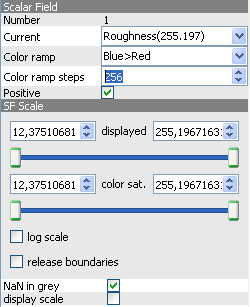
\includegraphics[width=0.4\textwidth]{images/Partie2_Interface/SFProperties}\\
\end{center}

Il est possible de rattacher plusieurs champs scalaires � un m�me nuage, mais un seul peut �tre actif (i.e. \textit{affich�}) � un instant donn�. Le nombre de champs scalaires associ�s � une entit� correspond d'ailleurs � la premi�re entr�e (\emph{Number}) de la section \emph{Scalar Field}.
\par
En dessous se trouve une liste d�roulante (\emph{Current}) permettant de sp�cifier le champ scalaire actif. Chaque champ scalaire � un nom unique. Celui-ci peut-�tre modifi� par l'utilisateur via la commande << Edit > Scalar fields > Rename >> (Cf. section\ref{subsection:sfRename}).
\par
Ensuite vient l'entr�e \emph{Color ramp} permettant de choisir la rampe de couleur\index{rampe!de couleurs} utilis�e pour l'affichage du champ scalaire sous forme de fausses couleurs (voir la section suivante pour plus de d�tails). Elle est suivie de l'entr�e \emph{Color ramp steps} qui permet de sp�cifier le nombre de couleurs diff�rentes utilis�es pour l'affichage en fausses couleurs. Par exemple, utiliser un nombre tr�s faible de couleurs sur une entit� dense permet d'obtenir un effet \textit{lignes de niveau}.
\par
Enfin, la derni�re entr�e de la section \emph{Scalar Field} est la case � cocher \emph{Postive} qui permet de sp�cifier si le champ scalaire doit �tre consid�r� comme strictement positif (auquel cas toutes les valeurs n�gatives sont consid�r�es comme �tant des valeurs invalides, de type \emph{NaN} = \textit{not a number}). Sinon, CloudCompare consid�re toutes les valeurs comme �tant valides. Cette propri�t� influe directement sur la mani�re dont la correspondance \textit{valeur scalaire - couleur} est calcul�e (voir ci-dessous).

\subsubsection{Rampe de couleurs (SF Scale)\label{Rampe-de-couleurs}\index{Rampe de couleur}}

La section \emph{SF Scale} est consacr�e � l'affichage du champ scalaire actif en fausses couleurs. Elle est en pratique toujours pr�sente si un champ scalaire est activ� (i.e. s�lectionn� dans la liste d�roulante \emph{Current} - voir ci-dessus).\\

Diff�rentes \index{rampes de couleurs} rampes de couleurs (ou encore \textit{�chelles de couleurs}) sont disponibles. Chacune correspond � un d�grad� de couleurs, la premi�re couleur �tant associ�e � la valeur minimale \emph{de saturation} du champ scalaire et la derni�re couleur � la valeur maximale \emph{de saturation}. Les couleurs interm�diaires sont associ�es aux valeur scalaires �quivalentes de mani�re lin�aire.\\
\par
Remarque : dans le cas d'un champ scalaire non strictement positif, il est possible de sp�cifier une �chelle de couleur avec saturation \emph{absolue}, auquel cas l'�chelle de couleur courante est coup�e en deux et est utilis�e de mani�re sym�trique pour les valeurs n�gatives ou positives (voir plus bas).

\begin{center}
\begin{tabular}{>{\raggedright}p{0.15\textwidth}>{\centering}p{0.8\textwidth}}
 & valeur minimale\hfill{}valeur maximale\tabularnewline
Bleu � rouge : & 
\includegraphics[angle=270,width=0.7\textwidth]{images/Partie2_Interface/ScalarRampBlueRed}\tabularnewline
Niveaux de gris : & 
\includegraphics[angle=270,width=0.7\textwidth]{images/Partie2_Interface/ScalarRampGrey}\tabularnewline
Rouge � jaune : & 
\includegraphics[angle=270,width=0.7\textwidth]{images/Partie2_Interface/ScalarRampYellowRed}\tabularnewline
Rouge � blanc : & 
\includegraphics[angle=270,width=0.7\textwidth]{images/Partie2_Interface/ScalarRampRedWhite}\tabularnewline
\end{tabular}
\par
\end{center}

\emph{CloudCompare} permet � l'utilisateur de param�trer finement \index{plage!de saturation}\index{plage!d'affichage} la mani�re dont les valeurs du champ scalaire courant sont affich�es en fausses couleurs (et ce de mani�re dynamique). Quatre valeurs cl�s sont modifiables interactivement :
\begin{center}
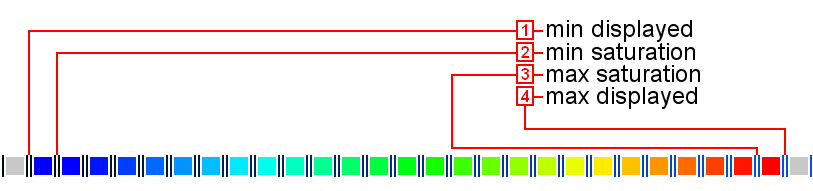
\includegraphics[width=1\textwidth]{images/Partie2_Interface/SFViewerCursors}
\par\end{center}
\begin{itemize}
\item \textbf{\textcolor{red}{1}} : \index{min!displayed value|see{plage d'affichage}}
Valeur minimale affich�e (\textsl{min displayed value}). Toutes les valeurs scalaires inf�rieures sont ignor�es (et sont alors consid�r�es comme �tant de type \emph{NaN} - voir plus bas).
\item \textbf{\textcolor{red}{2}} : \index{min!saturation value|see{plage de saturation}}
Valeur minimale de saturation (\textit{min saturation value}). Tous les valeurs inf�rieures (et donc comprises entre \textit{min displayed} et \textit{min saturation}) sont affich�es avec la (m�me) couleur, \og la
plus faible \fg{} de la rampe (ici en bleu).
\item \textbf{\textcolor{red}{3}} : \index{max!saturation value|see{plage de saturation}}
Valeur maximale de saturation (\textit{max saturation value}). Tous les valeurs sup�rieures (et donc comprises entre \textit{max saturation} et \textit{max displayed}) sont affich�es avec la (m�me) couleur, \og la
plus forte \fg{} de la rampe (ici en rouge).
\item \textbf{\textcolor{red}{4}} : \index{max!displayed value|see{plage d'affichage}}
Valeur maximale affich�e (\textit{max displayed value}). Toutes les valeurs scalaires sup�rieures sont ignor�es (et sont alors consid�r�es comme �tant de type \emph{NaN} - voir plus bas).\\
\end{itemize}
\par
La mani�re dont sont trait�es les \index{NaN|see{valeurs ignor�es}}\index{valeurs ignor�es}valeurs de type \emph{NaN} (valeurs invalides ou volontairement ignor�es par l'utilisateur via le r�glagle des valeurs \textit{min displayed} \textbf{\textcolor{red}{(1)}} et \textit{max displayed}) \textbf{\textcolor{red}{(4)}} se r�gle via la case � cocher \emph{Nan in grey}. Si celle-ci est coch�e, les points associ�s � ces valeurs scalaires sont affich�s avec une couleur grise par d�fault. Sinon ces points ne sont pas affich�s.\\

Les quatre valeurs cl�s pr�sent�es pr�c�demment permettent donc de d�finir plusieurs plages :
\begin{itemize}
\item les valeurs affichables, pour lesquelles les points sont effectivement affich�s en fausses couleurs. Le comportement en dehors de cette plage d�pend de la propri�t� \emph{Nan in grey}.
\item la plage de saturation, en dehors de laquelle la variation des couleurs est d�sactiv�e. La borne inf�rieure de cet intervalle est associ�e � la premi�re couleur de l'�chelle, la borne sup�rieure � la derni�re
couleur, et le reste des couleurs est r�parti lin�airement entre ces bornes.\\
\end{itemize}

\par
\emph{CloudCompare} v�rifie en permanence la coh�rence des valeurs saisies : on ne peut pas avoir \textbf{\textcolor{red}{(1)}}~$>$~\textbf{\textcolor{red}{(4)}} ni \textbf{\textcolor{red}{(2)}}~$>$~\textbf{\textcolor{red}{(3)}}. Toute modification valide d'une de ces valeurs est imm�diatement r�percut�e sur l'affichage, de mani�re interactive.Par d�faut les valeurs de saturation ne peuvent donc pas sortir des bornes 'min displayed value' \textbf{\textcolor{red}{(1)}} et 'max displayed value' \textbf{\textcolor{red}{(4)}}, et ces bornes sont impos�es par les donn�es elles-m�me (\emph{CloudCompare} calcule automatiquement ces bornes � partir des valeurs effectives du champ scalaire). Or, il arrive que pour des raisons esth�tiques ou pratiques l'utilisateur veuille voir apparaitre des bornes diff�rentes (en particulier au niveau de la repr�sentation graphique de l'�chelle de couleur dans la vue 3D), ou une saturation qui commence par exemple � partir de 0 dans tous les cas de figure. Il existe donc la propri�t� \emph{release boundaries} qui permet une fois activ�e de modifier manuellement les bornes 'min displayed' et 'max displayed' (il suffit pour cela de modifier manuellement les valeurs textuelles correspondantes en les rempla�ants par les nouvelles bornes d�sir�es).\\
\par
D'autres options sont disponibles :
\begin{itemize}
\item l'option \emph{log scale} permet d'afficher les fausses couleurs (et les valeurs textuelles correspondantes � l'�cran) selon une �chelle logarithmique.
\item comme �voqu� plus haut, dans le cas d'un champ scalaire non strictement positif, une option \emph{absolute saturation} apparait. Si l'utlisateur la coche, alors les valeurs 'min staturation' \textbf{\textcolor{red}{(2)}} et 'max saturation' \textbf{\textcolor{red}{(3)}} changent de sens : elles deviennent forc�ment positives et concernent � la fois les valeurs n�gatives et les valeurs positives (par sym�trie). La variation automatique des couleurs ne se passera donc qu'entre -'max saturation' et -'min stauration' et entre +'min stauration' et +'max stauration'. Les couleurs stagneront en dessous de -'max saturation' (couleur \textit{minimale} de la rampe - \textbf{bleu} typiquement), entre  -'min stauration' et +'min stauration' (couleur \textit{centrale} de la rampe - \textbf{vert} typiquement) et enfin au dessus de +'max saturation' (couleur \textit{maximale} de la rampe - \textbf{rouge} typiquement).\\
\end{itemize}

\par
Enfin, la rampe de couleurs avec les valeurs num�riques remarquables associ�es (min, max, valeurs de saturation, etc.) peut �tre affich�e � c�t� des entit�s dans la m�me vue 3D (cf. figure de la section \ref{Contexte-graphique}). Il faut cocher la case \emph{display scale} en fin de section \emph{SF scale}. Une seule rampe de couleur peut-�tre affich�e � la fois. De plus, si l'entit� associ�e est cach�e ou d�sactiv�e, la rampe de couleur ne sera pas affich�e.
\par


\subsection{Propri�t� de l'octree\index{octree, propri�t�s}\label{subsection:octreeProp}}

L'octree est indissociable du nuage de points auquel il est rattach�. Il s'agit d'une structure abstraite, disponible dans l'interface de \emph{CloudCompare} et affichable uniquement � titre informatif (elle peut aussi �tre supprim�e pour lib�rer de la m�moire si besoin). L'affichage de la structure propos� par \emph{CloudCompare} ne permet de visualiser qu'un niveau � la fois. Vous pouvez changer le \index{octree}niveau d'affichage de l'octree en incr�mentant/d�cr�mentant le champ \emph{Display level} de la section \emph{Octree}.

\begin{center}
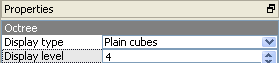
\includegraphics[width=0.4\textwidth]{images/Partie2_Interface/OctreeDisplayLevel}\\
\par
\end{center}

Les niveaux qui peuvent �tre affich�s vont de 1 � 10. Le niveau 0 ne peut �tre s�lectionn� (il n'est dailleurs en pratique jamais utilis�, pas m�me pour les calculs, puisque l'octree au niveau 0 correspond ni plus ni moins au nuage dans son int�gralit�, contenu dans une unique cellule).\\
\par
Il se peut que l'affichage ralentisse consid�rablement au del� d'un certain niveau de subdivision (en fonction des capacit�s de l'ordinateur sur lequel le programme s'ex�cute), � cause du nombre cons�quent d'�l�ments � afficher.\\
\par
L'octree peut �tre visualis� sous diff�rentes formes :
\begin{itemize}
\item Fil de fer (Wire) : \index{fil de fer, rendu}seules les arr�tes des cubes sont repr�sent�es (attention : lourd).
\item Points : chaque cube est repr�sent� par le centre de gravit� des points qui y sont inclus.
\item Surfacique (Plain cubes) : la surface des cubes est affich�e int�gralement (attention : tr�s lourd).\\
\end{itemize}
Le mode d'affichage courant de l'octree est controll� par la liste d�roulante \emph{Display type}.

\begin{center}
\includegraphics[width=0.4\textwidth]{images/Partie2_Interface/OctreeDisplayType}\\
\par
\end{center}

\subsection{Popri�t�s des �tiquettes standards\index{etiquette standard, propri�t�s}\label{subsection:stdLabelProp}}

Les �tiquettes 2D \textit{standards} sont des �tiquettes graphiques qui s'affichent en surimpression de la vue 3D et qui peuvent �tre associ�es � un ou plusieurs points (voir section \ref{subsection:standardLabel}).\\

\begin{center}
\includegraphics[width=0.4\textwidth]{images/Partie2_Interface/StandardLabelProperties}\\
\end{center}

Outre les options standards des objets affichables dans les vues 3D (voir section \ref{subsection:commonProperties}), ces �tiquettes poss�dent plusieurs champs regroup�s dans la section \emph{Label} :
\begin{itemize}
\item \emph{Body} - le corps de l'�tiquette (g�n�r� automatiquement). Pour information (et pour export, via copier-coller, si n�cessaire).
\item \emph{Show 2D label} - permet de cacher la partie 2D de l'�tiquette
\item \emph{Show 3D legend(s)} - permet de cacher la rappel du nom de l'�tiquette � c�t� du ou des points associ�s en 3D
\end{itemize}

\subsection{Popri�t�s des �tiquettes zone 2D\index{etiquette zone, propri�t�s}\label{subsection:zoneLabelProp}}

Les �tiquettes \textit{zone 2D} sont des �tiquettes graphiques qui s'affichent en surimpression de la vue 3D et qui sont associ�e � un point de vue (voir section \ref{subsection:zoneLabel}).\\

\begin{center}
\includegraphics[width=0.4\textwidth]{images/Partie2_Interface/ZoneLabelProperties}\\
\end{center}

Les �tiquettes \textit{zones 2D}, outre leur nom (qui appara�t en dessous du rectangle correspondant � l'�tiquette - ce nom est d'ailleurs modifiable comme pour toute entit�) n'ont qu'un bouton \emph{Apply} dans leurs propri�t�s. Celui-ci provoque l'application des param�tres de cam�ra associ�s � l'�tiquette dans la vue 3D (et donc cela force l'apparition de l'�tiquette, qui ne se dessine � l'�cran que si les param�tres de cam�ra courants co�ncident avec ceux de la cam�ra lors de la cr�ation de l'�tiquette).

\subsection{Popri�t�s des points de vues\index{point de vue, propri�t�s}\label{subsection:viewportProp}}

Il est possible � tout moment de sauver le point de vue courant (avec tous les param�tres de visualisation associ�s, comme la taille des points, etc.) via la commande << Display > Save viewport as object >> ou le raccourci clavier Ctrl+V. L'objet correspondant \textit{Viewport} se comporte exactement comme une �tiquette zone (mis � part qu'il n'a pas de repr�sentation associ�e).\\

\subsection{Popri�t�s des images\index{image}\label{subsection:imageProp}}

Des images (calibr�es ou non) peuvent �tre associ�es aux entit�s 3D. Dans le cas des images calibr�es (i.e. pour lesquelles on dispose de toutes les informations de calibrage intrins�ques et extrins�ques par rapport aux donn�es) il est possible de les afficher en surimpression de la vue 3D.\\
\par
Ces images peuvent �tre import�es via les formats E57, ICM ou encore via l'import de fichiers Bundler (OUT).\\

\begin{figure}[!htb]
\begin{center}
\includegraphics[width=0.9\textwidth]{images/Partie2_Interface/CalibratedImageGlobal}
\caption{\label{fig:CalibratedImageFig}Vue d'une image calibr�e en surimpression d'un nuage}
\end{center}
\end{figure}

\par
Les images ont toutes en commun la section \emph{Image} :
\begin{itemize}
\item \emph{Width} - largeur de l'image (en pixels)
\item \emph{Height} - hauteur de l'image (en pixels)
\item \emph{Alpha} - curseur permettant de r�gler la transparence (entre 0 et 100\%)
\end{itemize}

\par
La section \emph{Calibrated Image} est par contre reserv�e aux images calibr�es :
\begin{itemize}
\item \emph{Apply viewport} - change les param�tres de la vue 3D associ�e � l'image pour co�ncider avec ceux de l'appareil
\item \emph{f.o.v.} - \textit{field of view} ou ouverture angulaire (en degr�s)
\item \emph{Optical center} - centre optique
\item \emph{Orientation} - direction de vis�e
\item \emph{Angle} - Angle de rotation autour de l'axe de vis�e (en degr�s)\\
\end{itemize}

\subsection{Popri�t�s des capteurs laser (terrestres)\index{capteur, propri�t�s}\label{subsection:sensorProp}}

Les objets capteurs terrestres (\textit{Ground Based Lidar sensor}) ont une repr�sentation \textit{in situ} symbolique (un cube sur un tr�pied). Ils ont aussi une section propre dans la fen�tre de propri�t�s (section \emph{GBL sensor}) :
\begin{itemize}
\item \emph{dPhi} - le pas angulaire selon l'axe de rotation principal (en radians)
\item \emph{dTheta} - le pas angulaire selon l'axe de rotation secondaire (en radians)
\item \emph{Uncertainty} - l'incertitude en profondeur (utilis�e lors de la comparaison de nuages de points)
\item \emph{Display scale} - �chelle relative de la repr�sentation symbolique
\end{itemize}

\begin{figure}[!htb]
\begin{center}
\includegraphics[width=0.8\textwidth]{images/Partie2_Interface/gblSensorProperties}\\
\caption{\label{fig:gblSensorPropertiesFig}Repr�sentation symbolique d'un capteur laser terrestre}
\end{center}
\end{figure}


\section{Modification interactive des entit�s}

\subsection{Segmentation manuelle}\index{segmentation manuelle}
\label{subsection:graphicalSegmentation}

L'outil \textit{segmentation manuelle} (ou \textit{segmentation graphique interactive}) est accesible via l'ic�ne \includegraphics[height=15px]{images/Partie2_Interface/BtnSegment.png} de la barre d'outils sup�rieure (\textit{Main toolbar}). Il permet de "d�couper" manuellement � l'�cran la ou les entit�s s�lectionn�es.
\\
\par
Cet outil permet en effet de d�finir un contour � l'�cran (voir figure~\ref{fig:graphicalSegmentationExample}), puis de choisir si l'ont veut "garder" les points ou les triangles pr�sents � l'int�rieur ou � l'ext�rieur de
ce contour. Le processus est r�p�table � volont�, et les points/triangles rejet�s sont cach�s au fur et � mesure.
Si l'utilisateur valide sa segmentation, les entit�s s�lectionn�es sont chacune divis�es en deux : une partie correspondant aux points/triangles s�lectionn�s et l'autre avec les points/triangles restants.\\
\par
Note : dans le cas des maillages, les triangles pr�sents sur la fronti�re du contour ne sont pas \textit{d�coup�s} � proprement parler (on ne garde que les triangles dont les 3 sommets sont totalement inclus dans la fronti�re, et les autres triangles sont consid�r�s comme �tant \textit{� l'ext�rieur}).\\
\par
Deux types de contours sont disponibles :
\begin{itemize}
\item contour de type 'polyligne' : l'utilisateur peut d�finir les sommets successifs d'une polyligne par clics gauches successifs � l'�cran. Une fois le premier clic effectu�, CloudCompare fait apparaitre en temps r�el la forme de la polyligne en suivant le pointeur de la souris comme si celui-ci correspondait � un nouveau sommet. Un clic droit permet de figer le contour (n�cessaire pour effectuer une segmentation - voir ci-dessous). Enfin, tout clic gauche intervenant apr�s que le contour ait �t� fig� r�initialise celui-ci.
\item contour de type 'rectangle' : ce mode permet de d�finir des contours rectangulaires � l'�cran. Un simple clic droit permet de d�finir le premier coin du contour puis un second le coin oppos�. Il n'est pas n�cessaire de maintenir le bouton enfon�� entre les deux clics.\\
\end{itemize}

\begin{figure}[!htb]
\begin{centering}
\includegraphics[width=0.8\textwidth]{images/Partie2_Interface/graphicalSegmentation.jpg}
\caption{\label{fig:graphicalSegmentationExample}Outil de segmentation manuelle}
\end{centering}
\end{figure}

\par
En pratique, l'outil s'active dans la vue 3D courante (d'ailleurs seules les entit�s affich�es dans cette vue sont pris en compte par CloudCompare). L'interface principale de CloudCompare est \textit{gel�e} (la plupart des ic�nes et menus ne sont plus accessibles, mis � part les options d'affichage). Celle-ci est r�tablie quand l'utilisateur quitte l'outil (derni�re ic�ne � droite en forme de croix rouge).\\
Une barre d'ic�nes appara�t dans le coin haut-droit de la vue 3D :
\begin{itemize}
\item la premi�re ic�ne permet de mettre en pause la segmentation (ce qui permet de r�cup�rer le comportement normal de la souris et de faire tourner les entit�s 3D entre deux phases de contourage/d�coupe par exemple). Attention, si la segmentation est mise en pause, le contour actuellement dessin� dispara�t. Et si une segmentation est valid�e (voir plus bas), le processus est automatiquement mis en pause.
\item l'ic�ne suivante permet de choisir le mode de s�lection (polyligne - par d�faut - ou rectangulaire). En mode 'polyligne' il est toujours possible de d�finir un contour rectangulaire en maintenant la touche CTRL et le bouton gauche de la souris enfonc�s.
\item l'ic�ne suivante permet d'appliquer la segmentation selon le contour courant et en gardant affich�s les points \emph{� l'int�rieur} du contour. Les autres points sont alors cach�s et la segmentation est mise en pause. Le contour doit �tre ferm�.
\item l'ic�ne suivante permet d'appliquer la segmentation inverse (en gardant affich�s les points \emph{� l'ext�rieur} du contour).
\item l'ic�ne suivante correspond � une r�initialisation compl�te de la s�lection (tous les points redeviennent
visibles).
\item l'avant derni�re ic�ne permet de valider la segmentation globale et de quitter (les entit�s s�lectionn�es seront chacune scind�es en deux).
\item enfin la derni�re ic�ne permet d'annuler la segmentation et de quitter (aucune op�ration ne sera effectu�e).\\
\end{itemize}

\subsection{Rotation/translation manuelle}\index{translation manuelle}\index{rotation manuelle}
\label{subsection:graphicalTransformation}

L'outil \textit{transformation manuelle} (ou \textit{transformation graphique interactive}) est accessible via l'ic�ne \includegraphics[height=15px]{images/Partie2_Interface/BtnMove.png}. Il permet d'appliquer une rotation et/ou une translation manuelle aux entit�s s�lectionn�es.\\
\par
A l'instar de l'outil de segmentation interactive (voir ci-dessus), l'outil s'active dans la vue 3D courante (et seules les entit�s affich�es dans cette vue sont pris en compte par CloudCompare). L'interface principale de CloudCompare est aussi \textit{gel�e}. Trois ic�nes apparaissent en haut � droite de la vue 3D :
\begin{center}
\includegraphics[width=0.15\textwidth]{images/Partie2_Interface/BtnTranslateRotate}\\
\end{center}
\begin{itemize}
\item la premi�re permet de r�initialiser la transformation appliqu�es aux entit�s s�lectionn�es.
\item la seconde permet de valider la transformation et de quitter.
\item la derni�re permet d'annuler la transformation et de quitter.\\
\end{itemize}

\par
La transformation se fait interactivement avec la souris, en utilisant les m�mes conventions que pour la
transformation du point de vue (Cf. section~\ref{subsection:Interactivit�}) : le bouton gauche permet de tourner les entit�s (par rapport au centre de gravit� des boites englobantes de toutes les unit�s s�lectionn�es)
et le bouton droit permet de translater les entit�s dans le plan de l'�cran. Dans ce mode, seules les entit�s s�lectionn�es bougeront, les autres restant fixes. \\
\par
Note: si le processus est valid� par l'utilisateur, la transformation effectivement appliqu�e est affich�e dans la console (sous forme textuelle). \textit{Cette information peut-�tre r�cup�r�e par copier-coller.}



\section{Barres de progression}\index{progression, barre de}

Certains traitements ou op�rations de \emph{CloudCompare} n�cessitent un temps de traitement relativement long,
pouvant aller de quelques secondes � quelques minutes selon les capacit�s de l'ordinateur sur lequel l'application s'ex�cute, ainsi que le param�trage de la fonction et la complexit� inh�rente au traitement effectu�. La barre de progression est une fen�tre apparaissant durant les calculs non imm�diats, donnant un aper�u de l'�tat d'avancement du traitement.\\

\begin{center}
\includegraphics[width=0.2\textwidth]{images/Partie2_Interface/ProgressBar}\\
\end{center}

Parmi les commandes affichant une barre de progression, certaines laissent la possibilit� d'arr�ter\index{arr�ter un calcul} le calcul en cours d'ex�cution, via un bouton \emph{Cancel} (l'arr�t du processus n'est pas forc�ment imm�diat, le syst�me ne prenant en compte l'appui sur le bouton que lorsqu'il est suffisamment "disponible"). Lorsque ce bouton n'est pas visible, le traitement ne peut �tre interrompu avant la fin.

\section{Barres d'outils\index{outils, barre de}}

Vous trouverez ci dessous la liste des boutons disponibles dans les
diverses barres d'outils de \emph{CloudCompare}.

\begin{center}
\begin{longtable}{|>{\centering}m{0.07\textwidth}|>{\raggedright}m{0.4\textwidth}|>{\raggedright}m{0.5\textwidth}|}
\hline
\textbf{Bouton} & \textbf{Commande} & \textbf{Description}\tabularnewline
\hline
\endhead
\hline
\textbf{Bouton} & \textbf{Commande} & \textbf{Description}\tabularnewline
\hline
\endfirsthead
\hline
\hline
\multicolumn{3}{|c|}{Barre d'outils \emph{Main tools}}\tabularnewline
\multicolumn{3}{|c|}{\includegraphics[height=21px]{images/Partie2_Interface/MainToolBar}}\tabularnewline
\hline
\includegraphics[height=15px]{images/Partie2_Interface/BtnOpen} & \index{ouvrir des objets}Open & cf. section \ref{subsection:openFile} \tabularnewline
\hline
\includegraphics[height=15px]{images/Partie2_Interface/BtnSave} & Save & cf. section \ref{subsection:saveFile} \tabularnewline
\hline
\includegraphics[height=15px]{images/Partie2_Interface/pointPickingBtn} & Point picking & cf. section \ref{subsection:pointPicking}\tabularnewline
\hline
\includegraphics[height=15px]{images/Partie2_Interface/pointListPickingBtn} & Point list picking & cf. section \ref{subsection:pointListPicking}\tabularnewline
\hline
\includegraphics[height=15px]{images/Partie2_Interface/BtnClone} & Clone & cf. section \ref{subsection:clone}\tabularnewline
\hline
\includegraphics[height=15px]{images/Partie2_Interface/BtnFuse} & Fuse & cf. section \ref{subsection:fuse}\tabularnewline
\hline
\includegraphics[height=15px]{images/Partie2_Interface/BtnDelete} & Delete & Supprimer les objets s�lectionn�s\tabularnewline
\hline
\includegraphics[height=15px]{images/Partie2_Interface/BtnRegister} & Register & cf. section \ref{subsection:register} \tabularnewline
\hline
\includegraphics[height=15px]{images/Partie2_Interface/BtnAlign} & Align & cf. section\ref{subsection:align} \tabularnewline
\hline
\includegraphics[height=15px]{images/Partie2_Interface/BtnSubsample} & Subsample & cf. section \ref{subsection:subsample}\tabularnewline
\hline
\includegraphics[height=15px]{images/Partie2_Interface/BtnSamplePts} & Sample points & cf. section \ref{subsection:samplePoints} \tabularnewline
\hline
\includegraphics[height=15px]{images/Partie2_Interface/BtnCCDist} & Cloud/Cloud distance & cf. section \ref{subsection:cloud2cloudDist} \tabularnewline
\hline
\includegraphics[height=15px]{images/Partie2_Interface/BtnCMDist} & Cloud/Mesh distance & cf. section \ref{subsection:cloud2meshDist} \tabularnewline
\hline
\includegraphics[height=15px]{images/Partie2_Interface/BtnStatTest} & Statistical test & cf. section \ref{subsection:statisticalTest} \tabularnewline
\hline
\includegraphics[height=15px]{images/Partie2_Interface/BtnLabel} & Label connected components & cf. section \ref{subsection:labelConnectedComponents} \tabularnewline
\hline
\includegraphics[height=15px]{images/Partie2_Interface/BtnSegment} & Segment & cf. section \ref{subsection:graphicalSegmentation} \tabularnewline
\hline
\includegraphics[height=15px]{images/Partie2_Interface/BtnMove} & Translate/Rotate & cf. section \ref{subsection:graphicalTransformation} \tabularnewline
\hline
\hline
\multicolumn{3}{|c|}{Barre d'outils \emph{Scalar Field Tools}}\tabularnewline
\multicolumn{3}{|c|}{\includegraphics[height=21px]{images/Partie2_Interface/SFToolBar}}\tabularnewline
\hline
\includegraphics[height=15px]{images/Partie2_Interface/BtnHisto} & Show histogram & Afficher l'histogramme\index{histogramme} du champ scalaire courant\tabularnewline
\hline
\includegraphics[height=15px]{images/Partie2_Interface/BtnComputeStat} & Compute statistical parameters & cf. section \ref{subsection:computeStatParams} \tabularnewline
\hline
\includegraphics[height=15px]{images/Partie2_Interface/BtnFilterValue} & Filter by value & cf. section \ref{subsection:scalarFieldFilterByValue} \tabularnewline
\hline
\includegraphics[height=15px]{images/Partie2_Interface/BtnGradient} & Gradient & cf. section \ref{subsection:scalarFieldGradient} \tabularnewline
\hline
\includegraphics[height=15px]{images/Partie2_Interface/BtnGaussianFilter} & Gaussian filter & cf. section \ref{subsection:scalarFieldGaussianFilter} \tabularnewline
\hline
\includegraphics[height=15px]{images/Partie2_Interface/BtnSFRemove} & Delete current scalar field & Supprimer le champ scalaire actif du nuage s�lectionn�\tabularnewline
\hline
\includegraphics[height=15px]{images/Partie2_Interface/BtnDiff} & Difference & cf. section \ref{subsection:scalarFieldDiff}\tabularnewline
\hline
\hline
\multicolumn{3}{|c|}{Barre d'outils \emph{Plugins}}\tabularnewline
\multicolumn{3}{|c|}{\includegraphics[height=21px]{images/Partie2_Interface/PluginToolBar}}\tabularnewline
\multicolumn{3}{|c|}{\textit{peut contenir des �l�ments diff�rents que ceux list�s ici (en fonction des plugins disponibles)}}\tabularnewline
\hline
\includegraphics[height=15px]{images/Partie2_Interface/cc_qEDL} & Eye Dome Lighting (shader) & cf. section \ref{subsection:qHPR} \tabularnewline
\hline
\includegraphics[height=15px]{images/Partie2_Interface/cc_qSSAO} & Screen Space Ambient Occlusion (shader) & cf. section \ref{subsection:qSSAO} \tabularnewline
\hline
\includegraphics[height=15px]{images/Partie2_Interface/cc_qHPR} & Hidden Points Removal & cf. section \ref{subsection:qHPR} \tabularnewline
\hline
\includegraphics[height=15px]{images/Partie2_Interface/cc_qKinect} & Kinect Cloud Capture & cf. section \ref{subsection:qKinect} \tabularnewline
\hline
\includegraphics[height=15px]{images/Partie2_Interface/cc_qPCL} & PCL bridge & cf. section \ref{subsection:qPCL} \tabularnewline
\hline
\includegraphics[height=15px]{images/Partie2_Interface/cc_qPCV} & ShadeVis Ambient Occlusion & cf. section \ref{subsection:qPCV} \tabularnewline
\hline
\includegraphics[height=15px]{images/Partie2_Interface/cc_qPoissonRecon} & Poisson Surface Reconstruction & cf. section \ref{subsection:qPoissonRecon} \tabularnewline
\hline
\includegraphics[height=15px]{images/Partie2_Interface/cc_qRANSAC_SD} & Ransac Shape Detection & cf. section \ref{subsection:qRansacSD} \tabularnewline
\hline
\hline
\multicolumn{3}{|c|}{Barre d'outils \emph{Viewing Tools}}\tabularnewline
\multicolumn{3}{|c|}{\includegraphics[height=21px]{images/Partie2_Interface/ViewToolBar}}\tabularnewline
\multicolumn{3}{|c|}{\textit{cette barre d'outils est pr�sent�e en d�tail en section \ref{Options-affichage}}}\tabularnewline
\hline
\end{longtable}
\par\end{center}

Les barres d'outils peuvent �tre affich�es ou cach�es via le sous-menu << Display > Toolbars >>.

\section{Raccourcis clavier\index{raccourcis clavier}}

Voici les raccourcis clavier disponibles dans \emph{CloudCompare} :
\begin{center}
\begin{longtable}{|>{\raggedright}p{0.1\textwidth}|>{\raggedright}p{0.15\textwidth}|>{\raggedright}p{0.45\textwidth}|>{\raggedright}p{0.15\textwidth}|}
\hline
\textbf{Touche(s)} & \textbf{Commande} & \textbf{Action} & \textbf{Remarque}\tabularnewline
\hline
\endhead
\hline
\textbf{Touche(s)} & \textbf{Commande} & \textbf{Action} & \textbf{Remarque}\tabularnewline
\hline
\endfirsthead
\hline
F1 & Help & \index{aide}affiche l'aide de \emph{CloudCompare} & \tabularnewline
\hline
F2 & Rename & \index{renommer}renomme l'entit� s�lectionn�e & l'entit� doit �tre s�lectionn�e dans l'arbre de navigation\tabularnewline
\hline
F3 & Toggle centered perspective & \index{point de vue}active / d�sactive la projection prespective avec centre de rotation au niveau des entit�s & cf. section \ref{Options-affichage}\tabularnewline
\hline
CTRL~+~F3 & New 3D View & ouvrir une nouvelle vue 3D & \tabularnewline
\hline
F4 & Toggle viewer based perspective & \index{point de vue}active / d�sactive la projection prespective avec centre de rotation confondu avec l'oeil de l'utilisateur & cf. section \ref{Options-affichage}\tabularnewline
\hline
CTRL~+~F4 & \index{Vue 3D}Close 3D View & fermer la vue 3D courante & \tabularnewline
\hline
F5 & Refresh & rafra�chir l'affichage & \tabularnewline
\hline
F6 & Toogle sun light & \index{eclairage@�clairage}active / d�sactive la source lumineuse globale & cf. section \ref{Options-affichage}\tabularnewline
\hline
F7 & Toggle custom light & active / d�sactive la source lumineuse secondaire & cf. section \ref{Options-affichage}\tabularnewline
\hline
F8 & Toggle console& \index{console}affiche / cache la console & \tabularnewline
\hline
F11 & Full screen & \index{plein �cran}active / d�sactive l'affichage en plein �cran & \tabularnewline
\hline
CTRL~+~O & Open & \index{ouvrir un fichier}pour ouvrir un fichier & cf. section \ref{subsection:openFile} \tabularnewline
\hline
CTRL~+~S & Open & \index{sauver un fichier}pour sauver les entit�s s�lectionn�es  & cf. section \ref{subsection:saveFile} \tabularnewline
\hline
ALT~+~C & Set Unique Color & pour appliquer une couleur unique aux entit�s s�lectionn�es  & cf. section \ref{subsection:setUniqueColor} \tabularnewline
\hline
CTRL~+~V & Save Viewport & \index{sauver un point de vue}cr�� un objet \emph{Point de vue} correspondant au point de vue actuel (vue 3D active)  & cf. section \ref{subsection:viewportProp} \tabularnewline
\hline
V & Toggle entity visibility & inverse l'�tat d'affichage des entit�s s�lectionn�es & cf. section \ref{subsection:commonProperties} \tabularnewline
\hline
N & Toggle normals visibility & inverse l'�tat d'affichage des normales des entit�s s�lectionn�es & cf. section \ref{subsection:commonProperties} \tabularnewline
\hline
C & Toggle normals visibility & inverse l'�tat d'affichage des couleurs des entit�s s�lectionn�es & cf. section \ref{subsection:commonProperties} \tabularnewline
\hline
S & Toggle normals visibility & inverse l'�tat d'affichage du champ scalaire (courant) des entit�s s�lectionn�es & cf. section \ref{subsection:commonProperties} \tabularnewline
\hline
Del/Suppr & Delete & \index{supprimer}supprime les entit�s s�lectionn�es & \tabularnewline
\hline
SHIFT~+~left clic & Create 2D Label & \index{etiquette, cr�er}cr�� une �tiquette 2D standard associ�e au point d�sign� par le clic gauche (dans la vue 3D) & cf. section \ref{subsection:standardLabel} \tabularnewline
\hline
\end{longtable}
\par\end{center}


%---- Fonctions ----
\chapter{Fonctions}
\label{cha:Fonctions}

Dans ce chapitre sont d�taill�es les fonctions accessibles via le menu principal. Elles sont class�es par ordre d'apparition.

\section{Menu 'File'}
\label{sec:fileMenu}

\subsection{Open (file)}
\label{subsection:openFile}

\begin{figure}[!htb]
\begin{center}
\includegraphics[width=0.5\textwidth]{Partie3_Fonctions/fileOpenDlg.png}
\caption{\label{fig:fileOpenDlg}Interface de s�lection d'un fichier}
\end{center}
\end{figure}

\index{fichiers!ouvrir}
Permet de charger un fichier via une interface standard (figure~\ref{fig:fileOpenDlg}).\\
\par
Remarques :
\begin{itemize}
\item Raccourci clavier : \textcolor{red}{CTRL+O}
\item Si le chargement du fichier est r�ussi,  les entit�s correspondantes seront automatiquement affich�es dans la vue 3D active.
\item Le menu d�roulant \emph{Look in} / \emph{Regarder dans} permet d'acc�der � divers chemins usuels, ainsi qu'aux
chemins r�cemment utilis�s
\item Le menu d�roulant \emph{Files of type} / \emph{Fichiers du type} permet de choisir un filtre pour l'affichage des fichiers tout en donnant � CloudCompare une information sur le type de fichier � ouvrir (si le filtre est << All (*.*) >>, CloudCompare tentera de d�tecter automatiquement le bon type en fonction de son extension)
\end{itemize}

\subsubsection{Formats support�s}

Pour une liste des formats support�s, se r�f�rer � la section~\ref{section:fileFormats} des annexes.

\subsubsection{Moyen alternatifs de chargement de fichiers}

Il existe d'autres moyen de charger des fichiers dans CloudCompare:
\begin{itemize}
\item via la ligne de commande (voir annexes~\ref{subsection:commandeLine})
\item ou par \textit{drag \& drop} des fichiers (s�lectionn�s dans l'explorateur de Windows typiquement) directement dans une vue 3D de CloudCompare.\\
\end{itemize}

Note : dans ces deux cas CloudCompare tentera de deviner le format de fichier via leur extension.

\subsubsection{Cas des entit�s ayant des coordonn�es tr�s grandes}

Si l'entit� charg�e a des coordonn�es tr�s grandes (au moins une des composante sup�rieure � $10^6$), CloudCompare le signifiera � l'utilisateur et lui proposera de recentrer automatiquement l'entit� (voir figure~\ref{fig:recenterDialog}). Par d�faut le recentrage se fait sur le premier point lu dans le fichier. Ce m�canisme permet d'�viter de perdre de l'information car CloudCompare stocke les coordonn�es des points sur 32 bits.\\

L'information de recentrage est conserv�e avec le nuage de points (voir les propri�t�s du nuage en section~\ref{subsection:pointCloudProperties}). Elle sera conserv�e telle quelle si le fichier est sauvegard� dans le format binaire BIN. Et CloudCompare pourra m�me r�tablir les coordonn�es originales si l'entit� est sauv�e dans les formats supportants les coordonn�es sur 64 bits (LAS et E57) ou les formats ASCII (ASCII, OBJ, MA, VTK). Attention n�anmoins, certaines op�rations peuvent faire perdre cette information � CloudCompare (fusion avec un nuage non recentr�, etc.)\\

\begin{figure}[!htb]
\begin{center}
\includegraphics[width=0.7\textwidth]{Partie3_Fonctions/ccRecenterDialog.png}
\caption{\label{fig:recenterDialog}Interface de recentrage d'un nuage au chargement}
\end{center}
\end{figure}

Remarque: si l'utilisateur charge plusieurs fichiers � la fois (via une s�lection mutliple dans la boite de dialogue de chargement par exemple) et que CloudCompare d�tecte un d�passement de coordonn�es pour l'un des nuages, l'utilisateur a alors le choix d'appliquer un recentrage � chaque nuage individuellement ou � tous les nuages qui suivent (et qui n�cessitent un recentrage).


\subsection{Save (file)}
\label{subsection:saveFile}

\index{fichiers!sauvegarder}
\index{fichiers!formats}
Permet de sauvegarder dans un fichier l'entit� s�lectionn�e (voire plusieurs entit�s � la fois si le
format de fichier choisi le permet). Le fichier est d�sign� via une interface standard (figure~\ref{fig:fileOpenDlg}).\\
\par
Remarques :
\begin{itemize}
\item Le menu d�roulant \emph{Look in} / \emph{Regarder dans} permet d'acc�der � divers chemins usuels, ainsi qu'aux chemins r�cemment utilis�s
\item D�rouler le menu \emph{Files of type} permet de filtrer les fichiers du r�pertoire courant
affich�s et de d�signer le format de sauvegarde (en fonction du type et du nombre d'entit�s s�lectionn�es, diff�rents formats seront disponibles). Si le nom de fichier rentr� par l'utilisateur n'a pas d'extension, l'extension par d�faut pour ce format sera automatiquement rajout�e.
\end{itemize}


\section{Menu 'Edit'}
\label{sec:editMenu}

%Submenu Colors
\subsection{Colors > Set Unique}
\label{subsection:setUniqueColor}

\begin{figure}[!htb]
\begin{center}
\includegraphics[width=0.5\textwidth]{Partie3_Fonctions/colorSelectionDlg.png}
\caption{\label{fig:colorSelectionDlg}Interface de s�lection d'une couleur unique}
\end{center}
\end{figure}

\index{couleurs}
Permet de d�finir une couleur qui sera appliqu�e � tous les points/sommets des entit�s 3D s�lectionn�es. 
Le choix est manuel, et se fait via une interface classique proposant divers modes de s�lection (figure~\ref{fig:colorSelectionDlg}) :
\begin{itemize}
\item soit en choisissant une couleur \emph{basique} (en haut � gauche),
ou une couleur pr�c�demment sauvegard�e (\emph{custom} - en bas � gauche)
\item soit en cliquant sur la zone color�e (en haut � droite) et en faisant varier l'intensit� avec l'ascenseur
en d�grad� (� droite)
\item soit en rentrant manuellement les param�tres dans les trois champs HSV ou RGB (en bas � droite)
\end{itemize}
\par
Raccourci clavier : \textcolor{red}{ALT+C}


\subsection{Colors > Colorize}
\label{subsection:colorize}

\index{couleurs}
M�me interface que la fonction "Set Unique" (\ref{subsection:setUniqueColor} - voir ci-dessus).\\
\par
Cette fonction permet de modifier les couleurs actuelles des points par multiplication des composantes de la couleur actuelle par celles de la couleur s�lectionn�e.\\
\par
Soit $(r,g,b)$ les composantes rouge, vert et bleu d'un point, et $(r_m,g_m,b_m)$ la couleur � \textit{multiplier} :\\
	\[
		(r',g',b')=(r*\frac{r_m}{255},g*\frac{g_m}{255},b*\frac{b_m}{255})\\
	\]
Remarque : si l'entit� n'a pas de couleur, alors la fonction se comportera comme "Set Unique".

\subsection{Colors > Height Ramp}
\label{subsection:heightRamp}

\begin{figure}[!htb]
\begin{center}
\includegraphics[width=0.4\textwidth]{Partie3_Fonctions/heightRampDlg.png}
\caption{\label{fig:heightRampDlg}Interface de s�lection d'une rampe de couleur}
\end{center}
\end{figure}

\begin{figure}[!htb]
\begin{center}
\includegraphics[width=0.5\textwidth]{Partie3_Fonctions/HeightRamp.jpg}
\caption{\label{fig:heightRampExample}Exemple d'un d�grad� selon Z (couleurs par d�faut)}
\end{center}
\end{figure}

\index{couleurs}
L'utilisateur � le choix entre appliquer une rampe par d�faut (figure~\ref{fig:heightRampExample})
ou alors une rampe dont il d�finit les deux couleurs extr�mes (figure~\ref{fig:heightRampDlg}).
Il faut pour cela d�sactiver la case � cocher \emph{Use default ramp}. Les deux couleurs extr�mes du d�grad� peuvent alors �tre d�finies en cliquant sur les boutons color�s \emph{First color} et \emph{Second color} (qui
font appara�tre des interfaces de s�lection de couleur �quivalentes � celle de la m�thode \emph{Set Unique} - Cf. section~\ref{subsection:setUniqueColor}).\\
\par
Via la liste d�roulante \textit{direction}, l'utilisateur doit aussi d�finir selon quelle direction le d�grad� sera appliqu� (parmi les 3 directions principales : X, Y ou Z).


%Submenu Normals
\subsection{Normals > Compute}
\label{subsection:computeNormals}

\begin{figure}[!htb]
\begin{center}
\includegraphics[width=0.4\textwidth]{Partie3_Fonctions/computeNormalsDlg.png}
\caption{\label{fig:computeNormalsDlg}Interface pour le calcul des normales}
\end{center}
\end{figure}

\index{normales}
\textcolor{red}{Cette fonction ne permet pas de calculer des normales sign�es. Pour ceci utilisez la m�thode \textit{Estimate Normals and Curvature} de la librairie PCL via le plugin qPCL (voir \ref{subsection:qPCL}).}
\\
\par
Cette fonction permet de calculer les normales (non sign�es) d'un nuage de points.\\
\par
L'utilisateur peut sp�cifier le mod�le d'approximation locale de la surface parmi :
\begin{itemize}
\item Plane : plan aux moindres carr�s (le plus rapide)
\item Height function : quadrique (le plus pr�cis)
\item Triangulation : triangulation 2D$\frac{1}{2}$ de type Delaunay (int�rm�diaire)\\
\end{itemize}

L'utilisateur doit aussi sp�cifier la taille du voisinage pour la mod�lisation locale (\textit{local radius} : plus celui-ci est grand et plus le r�sultat sera lisse ... et le calcul lent).\\

Enfin, si une direction privil�gi�e pour les normales est disponible, l'utilisateur peut la sp�cifier pour aider CloudCompare � \textit{signer} les normales. Il faut activer la case � cocher \textsl{Prefered orientation} et sp�cifier une des 6 orientations par d�faut (-X,+X,-Y,+Y,-Z,+Z). Autrement, l'utilisateur peut tenter sa chance aupr�s de la m�thode \emph{Resolve direction} (Cf. section~\ref{subsection:resolveNormalsDirection}).

\subsection{Normals > Convert to HSV}
\label{subsection:convertToHSV}

Cette fonction permet de convertir les normales d'un nuage en couleur (voir figure \ref{fig:computeNormalsDlg}) via deux transformations successives :
\begin{itemize}
	\item une premi�re transformation des normales en indication de pendage (\textit{Strike and dip} en anglais - Cf. \href{http://en.wikipedia.org/wiki/Strike_and_dip}{wikipedia})
	\item puis une seconde transformation des informations de pendage vers l'espace HSV (\textit{Hue Saturation Value} ou  \textit{Teinte, Saturation, Valeur} en fran�ais) : $strike \rightarrow H$ ; $dip \rightarrow S$ ; $V = constante$.\\
\end{itemize}

\begin{figure}[!htb]
\begin{center}
\includegraphics[width=0.65\textwidth]{Partie3_Fonctions/convertToHSV.png}
\caption{\label{fig:computeNormalsDlg}Exemple de conversion de normales vers l'espace de couleur HSV}
\end{center}
\end{figure}

La m�thode cr�� le champ \textit{Couleur} si besoin (et sinon �crase la champ existant). Elle cache aussi automatiquement les normales.
\subsection{Normals > Invert}
\label{subsection:invertNormals}

\index{normales}
\index{inversion}
Inverse les normales des entit�s s�lectionn�es (nuages ou maillages).\\
\par
\emph{Note : cela permet notamment de corriger le probl�me du sens des triangles (direct ou indirect)
de certains maillages\index{maillage}}.

\subsection{Normals > Resolve direction}
\label{subsection:resolveNormalsDirection}

\index{normales}
\textcolor{red}{Cette fonction est une �bauche. Pour obtenir des normales sign�es, utilisez la m�thode \textit{Estimate Normals and Curvature} de la librairie PCL via le plugin qPCL (voir \ref{subsection:qPCL}).}\\

\par
Cette fonction tente de r�soudre le sens des normales d'un nuage de proche en proche, par propagation d'un ou plusieurs fronts sur le nuage (algorithme de type \emph{Fast Marching}).\\
\par
La propagation se fait sur une grille 3D (ici l'octree) et il faut donc choisir un niveau d'octree
auquel appliquer l'algorithme. Le choix du bon param�tre n'est malheureusement pas �vident, car un niveau
faible va entra�ner des cellules de taille importante, d'o� une propagation ais�e et rapide mais une mauvaise
prise en compte des circonvolutions locales, alors qu'un niveau �lev� va entra�ner l'inverse. De plus, plus
la propagation est difficile - i.e. par morceaux - plus le risque de voir des zones proches ayant des sens
oppos�s est forte. Il faut donc essayer l'algorithme � diff�rents niveaux d'octree, en commen�ant typiquement
� 5 ou 6, puis augmenter le niveau jusqu'� trouver une valeur satisfaisante.\\
\par
Note: la r�solution du sens des normales est au sens global pr�s, il peut donc �tre n�cessaire d'utiliser la fonction Invert\index{inversion} (Cf. section~\ref{subsection:invertNormals}) pour obtenir le r�sultat final recherch�.


%Submenu Octree
\subsection{Octree > Compute}
\label{subsection:computeOctree}

\index{octree}
Cette fonction calcule une structure octree (subdivision r�cursive de l'espace) pour le ou les nuages de points
s�lectionn�s. Une fois l'octree calcul� avec succ�s, il est affich� automatiquement (Cf. section~\ref{subsection:octreeProp}).\\
Remarque : l'utilisateur n'a jamais besoin de d�clencher le calcul de l'octree lui m�me, CloudCompare le fera automatiquement si besoin. Cette fonction permet juste d'afficher l'octree si celui-ci n'a pas d�j� �t� calcul�.

\subsection{Octree > Resample}
\label{subsection:resampleWithOctree}

\begin{figure}[!htb]
\begin{center}
\includegraphics[width=0.25\textwidth]{Partie3_Fonctions/resampleWithOctreeDlg.png}
\caption{\label{fig:resampleWithOctreeDlg}Interface pour r�-�chantillonnage par Octree}
\end{center}
\end{figure}

\index{echantillonner@�chantillonner!re-echantillonner@r�-�chantillonner}
Fonction de r�-�chantillonnage (grossier) d'un nuage. L'utilisateur sp�cifie un nombre approximatif de points (via
l'interface~\ref{fig:resampleWithOctreeDlg}), et \emph{CloudCompare} d�termine alors le niveau d'octree ayant un
nombre de cellules le plus proche de cette valeur. Le nuage r�-�chantillonn� est alors form� en rempla�ant chaque
cellule par un point \emph{repr�sentatif} (actuellement, le centre de gravit� des points pr�sents � l'int�rieur de
la cellule).\\
\par
Remarque : cette m�thode est diff�rente de la m�thode \emph{Subsample} (Cf. section~\ref{subsection:subsample})
car elle cr�e de nouveaux points 3D � des positions diff�rentes de celles des points d'origine, contrairement � la m�thode \emph{Subsample} qui ne fait que s�lectionner des points existants dans le nuage d'origine.


%Submenu Mesh
\subsection{Mesh > Delaunay 2D}
\label{subsection:computeDelaunay2DMesh}

\index{Delaunay|see{triangulation}}
\index{maillage!calculer � partir d'un nuage|see{triangulation}}
\index{triangulation}

Cette fonction permet de calculer un maillage 2D$\frac{1}{2}$ de type Delaunay � partir d'un nuage de points.\\
\par
Puisque la m�thode produit un maillage 2D$\frac{1}{2}$ � partir d'un nuage de points 3D, CloudCompare doit projeter pr�alablement celui-ci sur un plan avant de calculer sa triangulation associ�e. Ainsi cette m�thode est-elle d�clin�e en deux versions :
\begin{itemize}
\item \emph{axis aligned plane} : \emph{CloudCompare} estime que les altitudes sont port�es par l'axe principal Z et les points sont donc projet�s sur le plan (XY)
\item \emph{best LS plane} : approche plus g�n�rique, o� les points sont projet�s sur le plan interpolant le mieux
le nuage au sens des moindres carr�s (cette m�thode est particuli�rement adapt�e aux nuages assez \emph{plats} dont les altitudes ne sont pas forc�ment port�es par Z).
\end{itemize}

\subsection{Mesh > Best fitting quadric }
\label{subsection:computeBestFitQuadric}

\index{Quadrique}

\textcolor{red}{Cette m�thode est une m�thode \textit{recherche} (c.�.d. utilis�e pour des tests) non d�taill�e.}

\subsection{Mesh > Sample Points}
\label{subsection:samplePoints}
\index{echantillonner@�chantillonner!des points sur un maillage}

Cette fonction �chantillonne de mani�re al�atoire des points sur une surface d�crite par un maillage triangulaire (voir figure~\ref{fig:pointsSampling}).\\

\begin{figure}[!h]
\begin{center}
\includegraphics[width=0.9\textwidth]{Partie3_Fonctions/pointsSampling.jpg}
\caption{\label{fig:pointsSampling}Illustration du principe de l'�chantillonnage de points sur un maillage}
\end{center}
\end{figure}

\par
Cette fonction g�n�re un nouveau nuage de points. L'utilisateur � le choix via l'interface~\ref{fig:samplePointsOnMeshDlg} de sp�cifier :
\begin{itemize}
\item soit le nombre total de points d�sir� (approximatif).
\item soit la densit� par unit� de surface. Attention, la surface est exprim�e dans l'unit� implicite (au carr�) des sommets du maillage. Pour conna�tre la surface totale du maillage \index{surface, mesurer}, vous pouvez appeler pr�alablement la fonction << Mesh > Measure surface >> (section~\ref{subsection:measureSurface}).\\
\end{itemize}

\begin{figure}[!h]
\begin{center}
\includegraphics[width=0.3\textwidth]{Partie3_Fonctions/samplePointsOnMeshDlg.png}
\caption{\label{fig:samplePointsOnMeshDlg}Interface pour l'�chantillonnage de points sur un maillage}
\end{center}
\end{figure}


\subsection{Mesh > Smooth (Laplacian)}
\label{subsection:samplePoints}
\index{echantillonner@�chantillonner!des points sur un maillage}

Cette fonction lisse un maillage par approche de type Laplacien (voir figure~\ref{fig:laplacianSmooth}). Attention, ce type d'approche ne conserve pas la volume du maillage. De plus, les sommets du maillage sont d�plac�s.\\

\begin{figure}[!h]
\begin{center}
\includegraphics[width=0.9\textwidth]{Partie3_Fonctions/meshLaplacianSmooth.png}
\caption{\label{fig:laplacianSmooth}Maillage avant (� gauche) et apr�s (� droite) lissage de type \textit{Laplacien}}
\end{center}
\end{figure}

\par
Avant d'appliquer cette fonction, CloudCompare demande � l'utilisateur de d�finir deux param�tres :
\begin{itemize}
\item le nombre d'it�rations : plus les it�rations sont nombreuses, plus le lissage est fort... et plus la m�thode est longue.
\item la force du lissage � chaque it�ration : plus celle-ci est �lev�e, et plus le lissage est fort (ce qui peut permettre de diminuer le nombre d'it�rations - voir ci-dessus) mais plus les risques de probl�mes topologiques sont �lev�s.\\
\end{itemize}

\subsection{Mesh > Measure Surface}
\label{subsection:measureSurface}

\index{maillage}
\index{surface, mesurer}
Calcule la surface du maillage.\\
\par
Cette surface est exprim�e dans l'unit� implicite (au carr�) des sommets du maillage.

\subsection{Mesh > Scalar Field > Smooth}
\label{subsection:smoothMeshSF}

\begin{figure}[!htb]
\begin{center}
\includegraphics[width=0.9\textwidth]{Partie3_Fonctions/smoothAndEnhanceMeshSF.png}
\caption{\label{fig:smoothAndEnhanceMeshSF}Exemple de r�sultats obtenus avec les options \emph{smooth} et \emph{enhance} d'un champ scalaire port� par les sommets d'un maillage}
\end{center}
\end{figure}

\index{champ scalaire}
\index{lissage|see{filtrage}}
\index{filtrage}
Cette m�thode lisse spatialement les valeurs d'un champ scalaire port� par les sommets d'un maillage, en utilisant la topologie du maillage. La valeur scalaire au niveau d'un sommet est remplac�e par une moyenne (pond�r�e par la distance) des valeurs scalaires port�es par les sommets voisins.\\
\par
Remarque : cette fonction est beaucoup plus rapide que la fonction \emph{Gaussian filter}\index{filtrage!gaussien}
(section~\ref{subsection:scalarFieldGaussianFilter}) appliqu�e � un nuage de points non structur�. Elle ne permet par contre pas de r�gler la taille du \textit{noyau} de lissage.

\subsection{Mesh > Scalar Field > Enhance}
\label{subsection:enhanceMeshSF}

\index{contraste!r�haussage}

Cette m�thode r�hausse le \textit{contraste} d'un champ scalaire\index{champ scalaire} port� par les sommets d'un maillage, en utilisant la topologie du maillage. La valeur scalaire au niveau d'un sommet est modifi�e pour augmenter le contraste en prenant en compte les valeurs scalaires port�es par les sommets voisins (et leur distance respective).\\
\par
Cette fonction est l'inverse de \emph{Mesh > Scalar Field > Smooth} (voir section~\ref{subsection:smoothMeshSF}).


%Submenu Sensor
\subsection{Sensor > Ground-Based Lidar > Show depth buffer}
\label{subsection:showGBLDepthBuffer}

\index{profondeur, carte de}
\index{capteur}

\begin{figure}[!h]
\begin{center}
\includegraphics[width=0.7\textwidth]{Partie3_Fonctions/gblDepthBuffer.png}
\caption{\label{fig:gblDepthBuffer}Carte de profondeur associ�e � une entit� scanner (\textit{GBL sensor})}
\end{center}
\end{figure}


Affiche la carte de profondeur associ�e � un \emph{capteur} (GBL sensor - voir figure~\ref{fig:depthBuffer}). Elle correspond aux points 3D affich�s en fausses couleurs (en fonction de la distance par rapport au capteur) et projet�s dans le repaire polaire du scanner (li� � la rotation des mirroirs).

\subsection{Sensor > Ground-Based Lidar > Export depth buffer}
\label{subsection:exportGBLDepthBuffer}

\index{profondeur, carte de}
Cette fonction permet d'exporter la carte de profondeur associ�e � un \emph{capteur} sous la forme
d'un fichier texte.\\
\par
L'utilisateur est invit� � sp�cifier un nom de fichier dans lequel seront sauvegard�es toutes les
informations relatives � la carte de profondeur (voir section~\ref{subsection:depthMapFileDescription}).

\subsection{Sensor > Create}
\label{subsection:sensorProjection}

\index{capteur}
Cette fonction permet ce cr�er une entit� \emph{capteur} (de type scanner laser terrestre par d�faut) associ� � un nuage. Le nuage doit �tre s�lectionn� avant d'appeler cette fonction.\\
\par
Cela permet de mod�liser a posteriori le scanner qui a permis l'acquisition du nuage de points s�lectionn�. L'objet scanner peut-�tre utilis� notamment pour filter les points \textit{non comparables} lors du calcul de distance entre deux nuages de points (Cf. section~\ref{subsection:cloud2cloudDist}).\\

\begin{figure}[!htb]
\begin{center}
\includegraphics[width=0.4\textwidth]{Partie3_Fonctions/sensorProjectionDlg.png}
\caption{\label{fig:sensorProjectionDlg}Interface de param�trage pour la cr�ation d'un \emph{capteur}}
\end{center}
\end{figure}

Lors de la cr�ation d'un \emph{capteur}, de nombreux param�tres sont r�glables (via les diff�rents onglets de
l'interface~\ref{fig:sensorProjectionDlg}) :
\begin{itemize}
\item \emph{rotation order} : ordre des rotations du scanner (moteur, miroir). Nous utilisons ici les angles
$\theta$ et $\phi$ suivant les conventions habituelles des coordonn�es sph�riques :
$\theta$ repr�sente l'angle (le d�battement) horizontal du \emph{capteur},
$\phi$ repr�sente l'angle vertical du \emph{capteur}. Il existe deux choix actuellement :
$\theta$ puis $\phi$ (type \emph{GS} de \emph{Trimble}) ou $\phi$ puis $\theta$ (type \emph{Soisic} de \emph{Trimble}).
\item \emph{Position (center)/(X,Y,Z)} : position X,Y,Z du centre optique du scanner (exprim�e dans le r�f�rentiel
du nuage de point)
\item \emph{Position (center)/Sensor base} : �cart entre l'�metteur laser et le r�cepteur (utile pour un capteur
� triangulation comme le \emph{Soisic} typiquement).
\item \emph{Orientation} : rep�re du capteur exprim� par rapport au rep�re du nuage (trois vecteurs).
Par d�faut, la matrice form�e par ces trois vecteurs est lais�e � l'identit�, ce qui revient � avoir une
orientation \emph{droite} selon les 3 axes du rep�re courant.
\item \emph{Angular steps/dPhi} : pas angulaires (en degr�s) du capteur selon $\phi$.
\item \emph{Angular steps/dTheta} : pas angulaires (en degr�s) du capteur selon $\theta$.
\item \emph{Other/Uncertainty} : l'incertitude sur la mesure laser, en pourcentage (d�duite automatiquement
lors de la projection).
\item \emph{Other/Max. range} : la port�e maximale (d�duite automatiquement lors de la projection).\\
\end{itemize}
\par
Une fois les param�tres renseign�s, \emph{CloudCompare} cr�� un objet \emph{GBL sensor} associ� au nuage.
Celui-ci contient entre autre une carte de profondeur du nuage (voir section~\ref{subsection:showGBLDepthBuffer}).
Enfin l'objet \textbf{capteur} est affichable \emph{en situation} sous la forme d'un petit capteur 3D sch�matique
\index{afficher!des capteurs} (voir figure~\ref{fig:gblDepthBuffer} et section~\ref{subsection:sensorProp}).

\subsection{Sensor > Modify}
\label{subsection:modifySensor}

\index{capteur}
Permet de modifier les param�tres d'une entit� \emph{capteur} (\textit{GBL sensor}).\\
\par
L'utilisateur peut mettre � jour les param�ters de l'entit� \emph{capteur} via la m�me bo�te de dialogue que dans le cas de la cr�ation d'une entit� \emph{capteur} (voir~\ref{subsection:sensorProjection}).

\input{methods/computeSensorRanges}
\input{methods/computeSensorScatteringAngles}

%Submenu Scalar Fields
\subsection{Scalar Fields > Gradient}
\label{subsection:scalarFieldGradient}

\begin{figure}[!htb]
\begin{center}
\includegraphics[width=0.6\textwidth]{Partie3_Fonctions/sfGradientExample.jpg}
\caption{\label{fig:sfGradientExample}Interface de param�tre pour le calcul des normales}
\end{center}
\end{figure}

\index{champ scalaire}
\index{gradient}
Cette fonction permet de calculer les normes du gradient du champ scalaire actif.\\
\par \emph{CloudCompare} demande � l'utilisateur de pr�ciser si le champ scalaire correspond � une distance\index{distances} euclidienne (telles que les distances calcul�es entre deux nuages ou entre un nuage et un maillage - voir~\ref{subsection:cloud2cloudDist} ou \ref{subsection:cloud2meshDist}). Si oui, l'algorithme filtrera les valeurs aberrantes (qui sont alors facilement d�tectables car dans ce cas la valeur absolue du gradient ne peut �tre sup�rieure � 1).
\\
\par
Remarques :
\begin{itemize}
\item L'algorithme cr�e un nouveau type de champ scalaire (\emph{Gradient norms}).
\item Comme pour du traitement d'image 2D classique, le gradient permet notamment de mettre en valeur les zones de fortes variations du champ scalaire (on met ainsi en �vidence les bords des zones de changement par exemple - voir
figure~\ref{fig:sfGradientExample}).
\item Comme pour du traitement d'image 2D classique, il est souvent n�cessaire d'appliquer un filtre\index{filtrage!gaussien} gaussien aux donn�es avant et/ou apr�s un calcul du gradient (Cf. section~\ref{subsection:scalarFieldGaussianFilter}).
\item Le fait que la valeur de la norme du gradient ne soit jamais sup�rieure � 1 est vrai en r�alit� pour tout champ scalaire dont les valeurs varient proportionnellement � la distance entre les points (c'est donc le cas d'un champ de distances).
\end{itemize}

\subsection{Scalar Fields > Gaussian Filter}
\label{subsection:scalarFieldGaussianFilter}

\index{filtrage!gaussien}
\index{contraste!lissage|see{filtrage}}
\index{champ scalaire}

Application d'un filtre gaussien au champ scalaire actif.
\\
\par
L'utilisateur doit d�finir le noyau \emph{sigma} du filtre gaussien. Pour r�gler ce param�tre simplement, on peut se servir de l'octree\index{octree}, en prenant typiquement comme valeur la taille d'une cellule au niveau 8 pour un filtrage doux, 7 pour un filtrage relativement fort, etc. (la taille d'une cellule est affich�e au niveau de la console lorsqu'on affiche un \emph{rendu} du nuage via l'octree - Cf. section~\ref{subsection:octreeProp}).
\\
\par
Remarques :
\begin{itemize}
\item A partir de \emph{sigma}, on peut d�duire tr�s simplement le rayon de la sph�re en 3D d�limitant le voisinage qui sera consid�r� autour de chaque point. On calcule en effet pour chaque point la moyenne des valeurs scalaires de ses voisins, pond�r�e par la distance selon une loi gaussienne. Etant donn� que $3\sigma$ correspond � un �crasement du poids de 99,9\%, CloudCompare ne consid�re pas les points plus �loign�s.
\item Plus le noyau est grand, plus le calcul est lent.
\item Cette fonction est tr�s utile pour lisser le r�sultat d'un calcul du gradient\index{gradient} (section~\ref{subsection:scalarFieldGradient}) mais aussi d'un calcul de Portion de Ciel Visible (section~\ref{subsection:PCV}) sur un nuage de points par exemple.
\end{itemize}

\input{methods/scalarFieldBilateralFilter}
\subsection{Scalar Fields > Filter by Value}
\label{subsection:scalarFieldFilterByValue}

\begin{figure}[!htb]
\begin{center}
\includegraphics[width=0.32\textwidth]{Partie3_Fonctions/sfFilterByValueDlg.png}
\caption{\label{fig:sfFilterByValueDlg}Interface de param�trage pour le filtrage des points selon la valeur du champ scalaire actif}
\end{center}
\end{figure}

\index{champ scalaire}
\index{segmentation}
Cette fonction permet de segmenter un nuage en d�finissant un intervalle de valeurs scalaires (figure~\ref{fig:sfFilterByValueDlg}). Un nouveau nuage sera cr�� avec tous les points dont les valeurs scalaires (tir�es du champ scalaire actif) sont inclues dans cet intervalle. Lors de l'appel de la fonction, les valeurs par d�faut de la boite de dialogue correspondent aux valeurs \textit{min displayed} et \textit{max displayed} des param�tres d'affichage du champ scalaire actif (voir section~\ref{Champs-scalaires}).

\subsection{Scalar Fields > Arithmetic}
\label{subsection:scalarFieldDiff}

\index{champ scalaire}
\index{diff�rence}

\begin{figure}[!h]
\begin{center}
\includegraphics[width=0.3\textwidth]{Partie3_Fonctions/sfArtithmetic.png}
\caption{\label{fig:sfArtithmetic}Interface de la m�thode << Scalar Fields > Arithmetic >>}
\end{center}
\end{figure}

Cet outil permet d'effectuer des op�rations �l�mentaires (addition, soustraction, multiplication et division) entre des champs scalaires d'un m�me nuage.\\
\par
Pour appeler cette m�thode, un seul nuage doit �tre s�lectionn�. L'utilisateur doit alors choisir un champ scalaire $A$ et un champ scalaire $B$ ainsi qu'un type op�ration (voir figure~\ref{fig:sfArtithmetic}). Un champ scalaire $champ_{C} = champ_{A} op champ_{B}$ sera alors cr��.\\
\par
Remarque : le champ scalaire cr�� ($C$) est par d�faut sign�, m�me si les champs $A$ et $B$ sont non sign�s. Si cela est n�cessaire, l'utilisateur peut manuellement sp�cifier que ce champ scalaire est non sign� (voir section~\ref{Champs-scalaires} - case � cocher \emph{Postive}).


\subsection{Scalar Fields > Multiply}
\label{subsection:scalarFieldMultiply}
\index{champ scalaire}
\textcolor[rgb]{1.00,0.00,0.00}{Cette fonction n'est pas encore int�gr�e � la version 2.4 de \emph{CloudCompare}.}\\

\subsection{Scalar Fields > Convert to RGB}
\label{subsection:scalarFieldConvertToRGB}
\index{champ scalaire}
\index{couleurs}
Cette m�thode sauve le champ scalaire actif tel qu'affich� sous formes de couleurs (RGB).\\
\par
Si l'entit� poss�de d�j� des couleurs, \emph{CloudCompare} donne deux options � l'utilisateur : il est possible d'�craser les couleurs existantes ou de les \textit{multiplier} (voir l'outil << Colorize >> en section~\ref{subsection:colorize}).

\subsection{Scalar Field > Rename}
\label{subsection:sfRename}
\index{champ scalaire}

Cet outil permet de renommer le champ scalaire actif.


%Submenu Bounding-box
\subsection{Bounding-box > Fit principal components}
\label{subsection:bbPCA}
\index{boite englobante}

\textcolor{red}{Cette m�thode est une m�thode \textit{recherche} (c.�.d. utilis�e pour des tests).}

Cet outil permet de calculer une boite englobante \textit{optimale} par analyse en composantes principales.


%No submenu
\subsection{Point picking}
\label{subsection:pointPicking}

L'outil de \textit{picking} de points permet de s�lectionner un ou plusieurs points 3D (parmi les nuages affich�s) pour afficher des �tiquettes avec des informations diverses (notamment des mesures entre points : distance, angle, etc.).

\begin{figure}[!h]
\begin{center}
\includegraphics[width=0.7\textwidth]{Partie3_Fonctions/pointPicking.png}
\caption{\label{fig:pointPicking}Interface de \textit{picking} de points 3D}
\end{center}
\end{figure}

L'outil de picking de points s'active dans la vue 3D courante. Une barre d'ic�nes appara�t alors dans son coin haut-droit et l'interface principale de CloudCompare est \textit{gel�e} (la plupart des ic�nes et menus ne sont plus accessibles, mis � part les options d'affichage). Celle-ci est r�tablie quand l'utilisateur quitte l'outil (derni�re ic�ne � droite en forme de croix rouge).\\
En pratique, cet outil permet de cr�er des �tiquettes (voir section~\ref{etiquettes_2D} associ�e � un ou plusieurs points ou � une zone de l'�cran. Les 3 premi�res ic�nes de la barre d'outil permettent de cr�er une �tiquette li�e � un, deux ou trois points respectivement :
\begin{itemize}
\item 1 point : l'utilisateur s�lectionne un point et une �tiquette 2D standard appara�t avec les informations relatives � ce point (coordonn�es, indice dans le nuage, couleur, valeur scalaire active, etc.). 
\item 2 points : l'utilisateur s�lectionne deux points successivement (lors de la s�lection du premier point, l'�tiquette pr�c�dente appara�t) et des informations sur le segment ainsi d�fini sont alors affich�es (dont particuli�rement la distance entre les deux points).
\item 3 points : l'utilisateur s�lectionne trois points successivement (lors de la s�lection du premier point et du second point, les deux �tiquettes pr�c�dentes appara�ssent) et des informations sur le triplet de points ainsi d�fini sont alors affich�es (dont particuli�rement la normale et la surface du triangle correspondant ainsi que l'angle au niveau du premier point).
\item La quatri�me ic�ne permet de cr�er une �tiquette de type \emph{zone 2D}.
\item La cinqui�me ic�ne (disquette) permet de sauver l'�tiquette courante sous la forme d'une vraie entit� (autrement la cr�ation d'une nouvelle �tiquette ou quitter l'outil entraine la supression de l'�tiquette courante).
\item L'ic�ne suivante permet de r�initialiser l'outil (suppression de l'�tiquette courante).
\item Et enfin la derni�re ic�ne permet de quitter l'outil (suppression de l'�tiquette courante).
\end{itemize}



\subsection{Point list picking}
\label{subsection:pointListPicking}

L'outil de \textit{picking} d'une liste de points permet de s�lectionner interactivement une liste de points 3D d'un nuage (et de la sauver dans un fichier ou un nouveau nuage).

\begin{figure}[!h]
\begin{center}
\includegraphics[width=0.9\textwidth]{Partie3_Fonctions/pointListPicking.png}
\caption{\label{fig:pointPicking}Interface de \textit{picking} d'une liste de points 3D}
\end{center}
\end{figure}

L'outil de picking d'une liste de points s'active dans la vue 3D courante et pour un nuage de point qui doit �tre pr�alablement s�lectionn�. Une interface appara�t alors dans son coin haut-droit et l'interface principale de CloudCompare est \textit{gel�e} (la plupart des ic�nes et menus ne sont plus accessibles, mis � part les options d'affichage). Celle-ci est r�tablie quand l'utilisateur quitte l'outil (derni�re ic�ne � droite en forme de croix rouge).\\
Cet outil permet de s�lectionner une liste de points (par clicks successifs sur les points dans la vue 3D). Chaque point est ajout� � un tableau qui affiche les points dans leur ordre de s�lection avec 5 colonnes : l'indice du point dans la liste (cet indice appara�t aussi � c�t� du point dans la vue 3D) ; l'indice du point dans le nuage ; et les coordonn�es du point dans les 3 derni�res colonnes (X, Y et Z).\\
Une fois la liste form�e, il est possible de l'exporter avec l'ic�ne ``disquette'' (celle-ci fait appara�tre une liste d�roulante) :
\begin{itemize}
\item (x,y,z) : exporte la liste sous la forme d'un fichier de points (ASCII - un point par ligne) avec uniquement les coordonn�es des points (x,y,z)
\item (local index,x,y,z) : exporte la liste sous la forme d'un fichier de points (ASCII - un point par ligne) avec les coordonn�es des points pr�c�d�es de l'indice du point dans la liste (i,x,y,z)
\item (new cloud) : exporte la liste sous la forme d'un nouveau nuage de points\\
\end{itemize}

Les autres ic�nes permettent de :
\begin{itemize}
\item supprimer le dernier point dans la liste (premi�re ic�ne - ``fl�che'' qui se mord la queue)
\item valider la s�lection et fermer l'outil (ic�ne avec symbole vert). Dans ce cas les points de la liste sont conserv�s dans un sous groupe \textit{Picked points list} sous forme d'�tiquettes (cach�es en 2D par d�faut). Si une liste de points est associ�e � un nuage, ouvrir � nouveau l'outil avec ce nuage r�tablira automatiquement la liste dans le tableau (qui pourra donc �tre modifi�e � nouveau).
\item annuler la s�lection et fermer l'outil (ic�ne avec une croix rouge). Dans ce cas toutes les modifications apport�es sont annul�es (si une liste pr��xistait elle sera r�tablie).\\
\end{itemize}

Il est aussi possible de changer la taille des marqueurs de points (via le champ \textit{marker size} en bas � gauche) et aussi de changer l'indice de d�part de la liste (champ \textit{local start index}).\\


\subsection{Clone}
\label{subsection:clone}
\index{cloner}

Cr�� une nouvelle entit� identique en tout point � celle s�lectionn�e (et ind�pendante de cette derni�re).
Toute modification de l'entit� clon�e n'aura aucun impact sur l'entit�e d'origine (et inversement).\\

\par
Remarques :
\begin{itemize}
\item actuellement seuls les nuages et les maillages peuvent �tre clon�s.
\item attention � la consommation m�moire !
\end{itemize}

\subsection{Fuse}
\label{subsection:fuse}
\index{fusionner}

Fusionne deux (ou plus) entit�s s�lectionn�es. \textcolor{red}{Attention : les listes fusionn�es sont supprim�es � l'issue de cette op�ration.}\\

\par
Remarques :
\begin{itemize}
\item actuellement seuls les nuages ou les maillages peuvent �tre fusion�s.
\item toutes les caract�ristiques des entit�s sont conserv�es. Les entit�s ne poss�dant pas initialement telle ou telle caract�ristique (couleur, normale, champs scalaires, etc.) la gagneront, avec des �l�ments par d�faut (couleur blanche, normale nulle, valeur scalaire de type \textit{NaN}, etc.).
\end{itemize}

\subsection{Apply transformation}
\label{subsection:applyTransformation}

\begin{figure}[!h]
\begin{center}
\includegraphics[width=0.5\textwidth]{Partie3_Fonctions/applyTransformation.png}
\caption{\label{fig:applyTransformation}Interface de d�finition d'une transformation 3D (\textit{avec aide affich�e})}
\end{center}
\end{figure}

Cet outil permet � l'utilisateur de sp�cifier une transformation 3D (matrice $4\times4$ compos�e d'une matrice de rotation dans la partie sup�rieure � gauche et d'un vecteur translation dans la partie sup�rieure de la derni�re colonne). Cette transformation (ou son inverse si la case � cocher \textit{Apply inverse transformation} est activ�e) peut alors �tre appliqu�e aux entit�es s�lectionn�es.\\
\par
Remarques :
\begin{itemize}
\item une aide peut-�tre affich�e en appuyant sur le bouton en haut � gauche (voir figure~\ref{fig:applyTransformation}).
\item apr�s une transformation manuelle (voir section~\ref{subsection:graphicalTransformation}) ou un recalage de type ICP (voir section~\ref{subsection:register}) CloudCompare affiche dans la console la transformation appliqu�e aux entit�s. Cette transformation peut-�tre s�lectionn�e dans la console et r�cup�r�e - en \textit{copiant} le texte avec CTRL+C - puis \textit{coll�e} - CRTL+V - dans l'outil (attention, il faut faire attention aux premiers caract�res du texte coll� qui correspondent � l'heure du message et qui doivent donc �tre supprimm�s avant d'appliquer la transformation !). Ceci permet notamment soit d'annuler une transformation (en appliquant la transformation inverse) ou alors d'appliquer la m�me transformation � une autre entit�e apr�s un recalage (on peut en effet vouloir segmenter/nettoyer un nuage avant d'appliquer l'algorithme ICP - pour obtenir un meilleur recalage - puis appliquer la transformation obtenue au nuage d'origine).\\
\end{itemize}


\subsection{Multiply}
\label{subsection:multiply}

\begin{figure}[!h]
\begin{center}
\includegraphics[width=0.4\textwidth]{Partie3_Fonctions/Multiply.png}
\caption{\label{fig:multiplyDlg}Bo�te de dialogue pour la multiplication des coordonn�es}
\end{center}
\end{figure}

Multiplie les coordonn�es des points des entit�s s�lectionn�es par des constantes.\\
\par
L'utilisateur saisit les 3 coefficients multiplicateurs suivant chaque axe $(f_{X},f_{Y},f_{Z})$ via une bo�te de dialogue (voir~\ref{fig:multiplyDlg}).


\subsection{Subsample}
\label{subsection:subsample}

\begin{figure}[!h]
\begin{center}
\includegraphics[width=0.4\textwidth]{Partie3_Fonctions/subsamplingDlg.png}
\caption{\label{fig:subsamplingDlg}Interface de param�trage pour le sous-�chantillonnage de nuages}
\end{center}
\end{figure}

\index{echantillonner@�chantillonner!sous-echantillonner@sous-�chantillonner}
Fonction de sous-�chantillonnage des points d'un nuage.\\
\par
Diff�rentes m�thodes sont disponibles. Le choix (ainsi que le param�trage) se fait via une bo�te de dialogue (voir figure~\ref{fig:subsamplingDlg}) :
\begin{itemize}
\item \emph{Random} : sous-�chantillonnage al�atoire (les points sont tir�s au hasard). L'utilisateur choisit le nombre de points restants.
\item \emph{Space} : sous-�chantillonnage spatial. L'utilisateur choisit la densit� du nuage r�sultant via l'espace moyen inter-points maximal (valeur approximative).
\item \emph{Octree} : sous-�chantillonnage rapide via l'octree\index{octree}. On garde un point par cellule de
l'octree � un niveau donn� de subdivision. L'utilisateur choisit le niveau de subdivision (plus le niveau est faible et moins le nombre de points est important).\\
\end{itemize}
\par
Remarques :
\begin{itemize}
\item Le \textbf{sous}-�chantillonnage diff�re du \textbf{r�}-�chantillonnage (cf. section~\ref{subsection:resampleWithOctree}) dans le sens o� il ne cr�e pas de nouveaux points mais se contente de s�lectionner un sous-ensemble de points � partir du nuage source.
\item La m�thode de sous-�chantillonnage rapide via l'octree choisit le point le plus proche du centre dans chaque cellule. Ainsi l'�cart entre les points est � peu pr�s constant (si le nuage initial est suffisamment dense).
\end{itemize}

\subsection{Synchronize}
\label{subsection:synchronize}

\index{translation}
Fonction permettant d'aligner deux entit�s : elle applique simplement une translation � la deuxi�me entit�e pour faire co�ncider son centre de gravit� avec celui de la premi�re entit�.
\\
\par
Remarque : pour appeler cette fonction, il faut s�lectionner deux entit�s et uniquement deux.

\input{methods/toggleFeatures}

\section{Menu 'Tools'}
\label{sec:editMenu}

%Submenu Projection
\subsection{Tools > Projection > Unroll}
\label{subsection:unroll}

\begin{figure}[!htb]
\begin{center}
\includegraphics[width=0.6\textwidth]{Partie3_Fonctions/unrollDlg.png}
\caption{\label{fig:unrollDlg}Interface de param�trage pour l'outil de \emph{d�veloppement} d'un nuage}
\end{center}
\end{figure}

\index{developper@d�velopper}
\index{derouler@d�rouler|see{d�velopper}}
Cette fonction permet de \emph{d�velopper} sur un plan un nuage de point consid�r� comme �tant port� par une
forme de r�volution (cylindre ou un cone). Voir figure~\ref{fig:unrollExample}.
\\
\par
Il faut pour cela renseigner diff�rents param�tres d�finissant la forme de r�volution :
\begin{itemize}
\item le type (cylindre ou cone)
\item la dimension selon laquelle est positionn�e l'axe de d�veloppement (X, Y ou Z pour l'instant)
\item un point par lequel passe cet axe (dans le cas o� la checkbox \emph{auto axis} est s�lectionn�e, ce point est automatiquement
remplac� par le centre de gravit� du nuage)
\item le rayon du cylindre ou la base du cone
\item et l'angle d'ouverture du cone le cas �ch�ant\\
\end{itemize}
\par
\textcolor[rgb]{1.00,0.00,0.00}{Attention, pour optimiser la m�moire, cette fonction applique la transform�e
directement sur l'entit� s�lectionn�e ! Il peut �tre n�cessaire d'utiliser avant l'outil de clonage\index{cloner} -
voir section~\ref{subsection:clone}.}

\begin{figure}[!htb]
\begin{center}
\includegraphics[width=0.9\textwidth]{Partie3_Fonctions/unroll.jpg}
\caption{\label{fig:unrollExample}Exemple de r�sultat : nuage de points cylindrique (� gauche), et sa d�velopp�e
(� droite)}
\end{center}
\end{figure}

\subsection{Tools > Projection > Height Grid Generation}

\label{subsection:heightGridGeneration}

\index{projection!sur grille}
\index{grille|see{projection sur grille}}
Cette fonction permet de projeter un nuage de point sur une grille
r�guli�re suivant l'axe Z.\\

\begin{figure}[!h]
\begin{centering}
\includegraphics[width=0.45\textwidth]{Partie3_Fonctions/heightGridGenerationDlg.png}
\caption{\label{fig:heightGridGenerationDlg}Interface de param�trage pour
l'outil de projection d'un nuage sur une grille}
\end{centering}
\end{figure}

Une interface (figure~\ref{fig:heightGridGenerationDlg}) permet
de r�gler diff�rents param�tres :
\begin{itemize}
\item \emph{grid step} : le pas de la grille exprim� dans l'unit� des coordonn�es du nuage de points
\item \emph{type of projection} : ce param�tre peut prendre l'une des 2
valeurs suivantes :

\begin{itemize}
\item \textit{maximum height} : soit E$_{ij}$ le sous-ensemble de points du nuage
qui est projet� dans la case (i,j) de la grille. Pour chaque case (i,j)
de la grille, on retient comme altitude Z celle du point le plus haut
dans E$_{ij}$.
\item \textit{average height} : pour chaque case (i,j) de la grille, on
retient comme altitude Z l'altitude moyenne des points de E$_{ij}$.
\end{itemize}
\item \emph{fill empty cells with} : certaines cases de la grille r�guli�re
restent vides apr�s projection (aucun point du nuage ne s'y projette).
Ce param�tre indique avec quelle valeur l'on doit renseigner ces cases et peut prendre l'une des 3 valeurs suivantes :

\begin{itemize}
\item \textit{minimum height :} les cases vides sont renseign�es avec l'altitude
Z minimale parmi tous les points du nuage.
\item \textit{average height} : les cases vides sont renseign�es avec l'altitude
Z moyenne de tous les points du nuage.
\item \textit{maximum height} : les cases vides sont renseign�es avec l'altitude
Z maximale parmi tous les points du nuage.\\
\end{itemize}
\end{itemize}
\par
Cette fonction g�n�re deux fichiers (dans le r�pertoire du binaire
de \emph{CloudCompare} par d�faut) :
\begin{itemize}
\item \emph{height\_grid\_image.tiff} : l'image raster 2D cod�e sur 256 niveaux
de gris correspondant aux altitudes Z des points projet�s dans les cases de la grille ;
\item \emph{height\_grid\_text\_file.txt} : les donn�es de la grille sous un format ASCII (fichier exploitable
simplement par un programme).\\
\end{itemize}
\par
Voir figure~\ref{fig:heightGridGenerationExample} pour exemple de r�sultat produit par cette fonction.

\begin{figure}[!htb]
\begin{centering}
\includegraphics[width=0.95\textwidth]{Partie3_Fonctions/HeightGridImageExample.jpg}
\par\end{centering}
\caption{\label{fig:heightGridGenerationExample}Exemple de r�sultat : vue 3D � gauche, image 2D des hauteurs � droite}
\end{figure}


%Submenu Registration
\subsection{Tools > Registration > Register}
\label{subsection:register}

\begin{figure}[!htb]
\begin{center}
\includegraphics[width=0.4\textwidth]{Partie3_Fonctions/registrationDlg.png}
\caption{\label{fig:registrationDlg}Interface de param�trage pour l'outil de recalage de deux entit�s}
\end{center}
\end{figure}

\index{recalage}
Cette fonction permet de recaler deux nuages de points (algorithme \emph{"Iterative Closest Point"} de Besl et McKay, IEEE Trans. PAMI 1992).
\\
\par
\textcolor[rgb]{1.0,0.0,0.0}{Attention : pour que ce recalage fonctionne, il est n�cessaire que les deux nuages soit � peu pr�s align�s.\\}
\par
Cette fonction ne permet en aucun cas d'aligner des nuages positionn�s et orient�s de mani�re quelconque.
Son r�le est essentiellement d'affiner le recalage des nuages de points dont on estime qu'ils sont grossi�rement align�s. La fonction \emph{Align}
d�crite en section \ref{subsection:align} permet de faire en sorte que les nuages soient approximativement align�s et la
fonction \emph{Register} peut �tre utilis�e sur les deux nuages r�sultant de cette fonction \emph{Align}.
\\
\par
La zone sup�rieure (\emph{Model and Data}) de la fen�tre de param�trage permet � l'utilisateur d'attribuer interactivement le r�le\index{role@r�le}
de chaque entit�. Le \emph{Model} est le nuage de r�f�rence (qui ne bouge pas) et \emph{Data} d�signe le nuage � recaler (il pourra bouger si n�cessaire).
Pour aider l'utilisateur, \emph{CloudCompare} force la coloration des entit�s et leur affichage (\emph{model} en rouge et \emph{data} en jaune)
selon le m�me principe que l'interface de choix des r�les avant un calcul de distances (voir paragraphe ci-dessous).
Un bouton permet d'intervertir ces roles si besoin (\emph{swap}).
\\
\par
La partie inf�rieure (\emph{Registration parameters}) correspond aux param�tres de l'algorithme de recalage en tant que tel.
Voici leur d�tail :
\begin{itemize}
\item \emph{Stop criterion} : l'utilisateur choisit soit un nombre d'it�rations fixe (ceci permet d'�viter un temps de calcul trop long,
mais ne garantit pas la qualit� du recalage) ou au contraire une diminution de l'erreur minimale entre deux it�rations
pour justifier d'autres it�rations : autrement, l'algorithme s'arr�te, estimant que le gain en pr�cision est insuffisant
(ce qui garantit une meilleure qualit� mais peut prendre potentiellement beaucoup de temps).
\item \emph{Enable furthest point removal} : heuristique adapt�e au recalage d'entit�s l�g�rement diff�rentes (puisque
\emph{CloudCompare} est justement fait pour comparer des nuages potentiellement diff�rents, alors que l'algorithme est pens�
pour recaler des nuages repr�sentant les m�mes objets !). Cet heuristique consiste � �carter les points
trop �loign�s � chaque it�ration du recalage (et ce de plus en plus), pour �viter que les diff�rences entre les nuages
ne fassent trop \emph{glisser} la position finale du nuage recal�).

\textcolor[rgb]{1.0,0.0,0.0}{Donc cette option ne doit pas �tre coch�e si les deux nuages repr�sentent les m�mes objets.}
\end{itemize}

\subsection{Tools > Registration > Align}
\label{subsection:align}

\begin{figure}[!htb]
\begin{center}
\includegraphics[width=0.6\textwidth]{Partie3_Fonctions/alignDlg.png}
\caption{\label{fig:alignDlg}Interface de param�trage pour l'outil de recalage grossier de deux entit�s}
\end{center}
\end{figure}

Cette fonction permet de recaler\index{recalage}\index{aligner des nuages|see{recalage}} grossi�rement deux nuages de points (algorithme \emph{"4 points Congruent Sets For Robust
Registration"} de Aiger, Mitra et Cohen-Or, Siggraph 2008).
\\
\par
Une premi�re zone de saisie (en haut � gauche) permet d'indiquer les 2 nuages � recaler et leurs r�les\index{role@r�le}
respectifs (\emph{Model and Data} : le \emph{Model} est le nuage de r�f�rence (qui ne bouge pas) sur lequel viendra s'aligner (si possible)
le nuage \emph{Data}.
Comme le recalage calcul� est un recalage rigide, seules des translations et des rotations peuvent �tre appliqu�es
� l'ensemble du nuage \emph{Data}.
Plusieurs autres param�tres doivent �tre renseign�s par l'utilisateur pour une utilisation optimale de cette m�thode.
\\
\par
\emph{Sampling} : cette zone concerne l'�tape pr�alable de sous-�chantillonnage\index{echantillonner@�chantillonner!sous-echantillonner@sous-�chantillonner}
des nuages de points. Cela permet d'am�liorer sensiblement l'efficacit� de l'algorithme.
En effet, quelques dizaines de milliers de points suffisent g�n�ralement � obtenir un bon
recalage, alors que la complexit� de l'algorithme augmente rapidement en fonction du nombre de points. L'utilisateur devrait toujours
chercher � minimiser le nombre de points pris en compte, quitte � relancer l'algorithme avec plus de points si besoin.
Voici les param�tres du sous-�chantillonnage :
\begin{itemize}
\item \emph{Method} : m�thode de sous-�chantillonnage (voir section~\ref{subsection:subsample}). S�lectionnez \emph{None} pour ne pas sous-�chantillonner
\item \emph{Model} : un slider et/ou un champ avec variateur permet de choisir le nombre de points conserv� pour le nuage de r�f�rence
\item \emph{Data} : idem, un slider et/ou un champ avec variateur permet de choisir le nombre de points conserv� pour le nuage recal�\\
\end{itemize}
\par
\emph{Registration parameters} : cette zone correspond aux param�tres de l'algorithme de recalage en tant que tel.
Nous expliquons en d�tail ces param�tres :
\begin{itemize}
\item \emph{Number of trials} : l'algorithme proc�de par essais successifs et ne retient que celui ayant fourni le meilleur r�sultat.
Ce champ permet de choisir le nombre d'essais � effectuer. Plus la valeur saisie est grande, plus le calcul sera long, mais plus la
probabilit� d'obtenir de bons r�sultats sera �lev�e. Il peut donc �tre n�cessaire d'adapter ce param�tre en fonction du nombre de points
composant les nuages pour obtenir un bon alignement dans un temps raisonnable. Pour donner un ordre d'id�e, une cinquantaine d'essais
pour recaler deux nuages de 5000 points chacun permet d'obtenir un r�sultat convenable en quelques minutes (de l'ordre de 2 � 5 minutes,
tout d�pend de l'ordinateur sur lequel le programme s'ex�cute).
\item \emph{Overlap} : ce param�tre, compris entre 0.0 et 1.0, correspond � une estimation du taux de recouvrement entre les deux nuages
lorsqu'ils sont correctement align�s. Un taux de recouvrement de 1 signifie que les deux nuages se recouvrent quasiment enti�rement, 0
signifiant que les nuages sont disjoints (dans ce cas, le recalage n'a pas beaucoup de sens). Une estimation tr�s approximative
du recouvrement est en g�n�ral suffisante, il ne s'agit en aucun cas de renseigner avec pr�cision la valeur effective.
\item \emph{Delta} : ce param�tre correspond � une estimation a priori de la distance moyenne qui existera entre les points des deux nuages
apr�s qu'ils aient �t� recal�s. Il sert de crit�re d'arr�t et agit comme une tol�rance � l'erreur : plus il est proche de 0, plus on contraint
les nuages � �tre proches, mais plus la probabilit� de trouver une bonne solution est faible. En principe, si \emph{Delta} vaut z�ro, le 
programme ne pourra pas trouver d'alignement entre les deux nuages. En r�gle g�n�rale, pour obtenir de bons r�sultats, \emph{Delta} doit 
correspondre � la r�solution (inverse de la densit�) du nuage de r�f�rence. L'interface propose un bouton \emph{Estimate} qui permet 
d'estimer de mani�re automatique ce param�tre en se basant sur un calcul de la densit� moyenne du nuage de r�f�rence.
\item \emph{Limit max. number of candidates} : lorsque ce champ est activ� (pour cel�, cocher la case qui y est associ�), il est possible de fixer
le nombre maximal de candidats que le programme est autoris� � traiter pour chaque essai. En effet, lors d'un essai, le processus recherche
dans le nuage servant de donn�es des ensembles de points pouvant mener � un bon recalage. Ces ensembles sont calcul�s en fonction des param�tres cit�s
pr�c�demment, et le programmme peut �tre amen� � trouver un nombre �norme de candidats (quelques centaines de milliers d'ensembles). Ce param�tre permet
de ne s�lectionner parmi ces candidats que ceux qui sont consid�r�s comme �tant les meilleurs, et donc de raccourcir consid�rablement le temps de
traitement de chaque essai. En contrepartie, on se prive potentiellement de trouver le meilleur recalage � cause de l'heuristique utilis�e pour retenir
les meilleurs candidats. Lorsque ce champ est d�sactiv�, le nombre maximal de candidats est illimit�, ce qui peut conduire � de tr�s grands temps de calcul.
\end{itemize}

\begin{figure}[!htb]
\begin{center}
\includegraphics[width=0.8\textwidth]{Partie3_Fonctions/alignExample}
\caption{\label{fig:alignExample}Alignement de deux nuages se recouvrant partiellement.
A gauche la configuration initiale, � droite le r�sultat du recalage avec un recouvrement estim� � 90\%
(\emph{Overlap}~$=\:0,9$) et une vingtaine d'essais (\emph{Number of trials}).}
\end{center}
\end{figure}

\par
Les param�tres \emph{Delta} et \emph{Overlap} n�cessitent donc que l'utilisateur ait une id�e a priori de ce que seront les nuages apr�s avoir
�t� align�s.
\\
\par
La figure \ref{fig:alignExample} pr�sente le r�sultat obtenu en alignant deux scans d'une peluche relev�s sous deux angles sensiblement
diff�rents. En th�orie, la fonction \emph{Align} est capable de traiter des nuages avec des taux de recouvrement beaucoup plus faibles que ceux
pr�sent�s en exemple.
\\
\par
Les alignement calcul�s via cette fonctionnalit� d�pendent grandement de la configuration des nuages � traiter. En effet, leur g�om�trie
ainsi que le degr� de ressemblance les rendent plus ou moins facilement comparables. De ce fait, il se peut que les r�sultats fournis dans
certains cas semblent relativement mauvais. Dans ces situations, vous pouvez alors utiliser la fonction de recalage fin d�crite en
section~\ref{subsection:register}. Il est m�me conseill�, de mani�re g�n�rale, d'avoir recours au recalage fin apr�s utilisation de cette
fonctionnalit�.
\\
\par
\textcolor[rgb]{1.0,0.0,0.0}{Cette fonction cr�e une copie du nuage \emph{Data} align� sur le nuage \emph{Model}.
Il n'est donc pas n�cessaire de cloner les nuages avant, puisqu'ils ne sont pas modifi�s directement.}


%Submenu Distance
\subsection*{Choix des r�les (interface g�n�rique)}
\label{subsection:chooseRole}

\index{role@r�le}

\par
\normalsize
Cette interface g�n�rique (figure~\ref{fig:chooseRoleDlg}) est utilis�e par toutes les m�thodes de calcul de distance,
ainsi qu'un certain nombre d'autres m�thodes (qui l'utilisent comme telle ou sous une forme �quivalente). Elle permet
� l'utilisateur d'attribuer interactivement un r�le sp�cifique � deux entit�s qui ont �t� s�lectionn�es en m�me temps.
\emph{CloudCompare} force la coloration des entit�s en fonction du r�le qui leur a �t� affect�. 
Dans le cas des distances par exemple, le nuage de r�f�rence est repr�sent� en jaune et le nuage � comparer 
(celui qui portera le champ scalaire apr�s calcul), en rouge. 
Un bouton \emph{swap} permet d'intervertir le r�le (et donc la coloration) des deux entit�s.

\begin{figure}[!h]
\begin{center}
\includegraphics[width=0.9\textwidth]{Partie3_Fonctions/chooseRoleDlg.jpg}
\caption{\label{fig:chooseRoleDlg}Interface standard de choix des r�les des entit�s}
\end{center}
\end{figure}

\subsection{Tools > Distances > Cloud/Cloud dist.}
\label{subsection:cloud2cloudDist}

\begin{figure}[!htb]
\begin{center}
\includegraphics[width=0.3\textwidth]{Partie3_Fonctions/cloud2cloudDistDlg.png}
\caption{\label{fig:cloud2cloudDistDlg}Interface de param�trage pour le calcul de distances entre deux nuages de points}
\end{center}
\end{figure}

Cette fonction permet de calculer les distances\index{distances} (approximatives ou exactes) entre deux nuages de points.
\\
\par
Lors de l'appel de cette fonction, et apr�s avoir choisi le r�le\index{role@r�le} de chaque nuage
(Cf. section~\ref{subsection:chooseRole}), un premier calcul de distances approximatives entre les deux nuages
(distances de Chanfrein, calcul�es via l'octree) est effectu� de mani�re automatique. Cela permet d'afficher
dans la partie sup�rieure de l'interface~\ref{fig:cloud2cloudDistDlg} (\emph{Approx. results}) diverses
informations sur les distances qui peuvent alors �tre calcul�es pr�cis�ment.
\\
\par
Ces informations sont :
\begin{itemize}
\item \emph{Min. dist.} : distance (approximative) minimale
\item \emph{Max. dist.} : distance (approximative) maximale
\item \emph{Mean. dist.} : distance (approximative) moyenne
\item \emph{Sigma} : �cart type
\item \emph{Max relative error} : erreur relative maximale de l'approximation (exprim�e sous forme d'une fonction de
$d$ - la distance, car cette erreur est d�pendante de la distance r�elle des points, et g�n�ralement d�cro�t
rapidement quand $d$ cro�t, ce qui veut dire que l'approximation de la distance minimale est g�n�ralement tr�s
mauvaise, mais celle de la distance maximale peut-�tre assez fiable).\\
\end{itemize}
\par
L'utilisateur peut enfin afficher l'histogramme des distances approximatives calcul�es (en appuyant sur l'icone
\includegraphics{images/Partie3_Fonctions/cc_histogramIcon}), mais celui-ci est g�n�ralement assez peu d�taill� �tant donn� le principe du calcul des distances de
Chanfrein via l'octree.
\\
\par
La partie inf�rieure (\emph{Precise results}) permet le param�trage du calcul pr�cis des distances.
L'utilisateur peut saisir les valeurs suivantes :
\begin{itemize}
\item \emph{Local model} : indique quelle \index{modele@mod�le}une mod�lisation locale sera appliqu�e au nuage de r�f�rence pour am�liorer la pr�cision
du calcul de distance nuage � nuage (dans une certaine mesure). Cette technique permet une am�lioration de la pr�cision globale (et non forc�ment locale).
Cette am�lioration d�pend du mod�le choisi, et se fait au prix d'un certain ralentissement de la fonction (qui d�pend lui aussi du
mod�le choisi) :
\begin{itemize}
\item {NONE} : pas de mod�lisation locale (comportement par d�faut), on calcule la distance au point le plus proche.
\item {Least Square Plane} : approximation locale du nuage par un plan (ajust� aux moindres carr�s) - peu pr�cis mais rapide.
\item {2D$\frac{1}{2}$ triangulation} : approximation locale du nuage par une triangulation de Delaunay 2D$\frac{1}{2}$ (apr�s
projection des points sur un plan ajust� aux moindres carr�s) - vitesse et pr�cision interm�diaires.
\item {Height Function} : approximation locale du nuage par une fonction de hauteur du type $z = ax+by+cx^2+dy^2+exy$ (l� encore,
apr�s projection des points sur un plan ajust� aux moindres carr�s) - meilleure pr�cision mais vitesse r�duite.
\end{itemize}
\item \emph{Max. dist} : permet � l'utilisateur de d�finir une distance au del� de laquelle il n'est pas n�cessaire de calculer
une distance pr�cise. Cela permet d'am�liorer fortement les performances du calcul, en particulier sur des nuages ayant peu
de zones communes (en �vitant ainsi de calculer des distances �loign�es - les plus co�teuses - alors que leur connaissance
pr�cise est g�n�ralement inutile). \emph{Les points concern�s conservent alors leur distance approximative. Les informations
affich�es dans la partie sup�rieure peuvent grandement aider � fixer cette valeur limite.}
\item \emph{Octree level} : \index{octree}ce param�tre de l'algorithme est normalement adapt� au mieux par \emph{CloudCompare}, mais il est
possible de le forcer au cas o� l'heuristique de d�termination est d�faillante.\\
\end{itemize}
\par
Remarques :
\begin{itemize}
\item Cette fonction rajoute un champ scalaire \emph{C2C Distances} au nuage de r�f�rence.
\item \textcolor[rgb]{1.00,0.00,0.00}{Pour calculer les distance pr�cises il est n�cessaire d'appuyer sur le bouton rouge \emph{Compute}.}
Autrement, seules les distances approximatives sont conserv�es.
\item Toutes les distances calcul�es par cette fonction ou rentr�es en param�tre sont exprim�es dans la m�me
unit� que les coordonn�es du nuage de points (il n'y a plus d'unit� explicite dans \emph{CloudCompare 2.1}).
\end{itemize}

\subsection{Tools > Distances > Cloud/Mesh dist.}
\label{subsection:cloud2meshDist}

\begin{figure}[!htb]
\begin{center}
\includegraphics[width=0.4\textwidth]{Partie3_Fonctions/cloud2MeshDistExample.jpg}
\caption{\label{fig:cloud2MeshDistExample}Exemple de r�sultat de calcul de distances entre un nuage et un maillage}
\end{center}
\end{figure}


Cette fonction permet de calculer les distances\index{distances} (approximatives ou exactes) entre un nuage de points et un maillage.
\\
\par
Cette fonction est largement �quivalente au calcul de distances entre nuages (section~\ref{subsection:cloud2cloudDist}) mis � part
quelques d�tails :
\begin{itemize}
\item si un seule des deux entit�s s�lectionn�es est un maillage, le choix des r�les (section~\ref{subsection:chooseRole}) n'est
pas n�cessaire (le maillage est forc�ment l'entit� de r�f�rence).
\item si les deux entit�s s�lectionn�es sont des maillages, les sommets de l'entit� \emph{compar�e} seront utilis�s en guise de
\emph{nuage}. Il peut �tre int�ressant d'utiliser la fonction d'�chantillonnage\index{echantillonner@�chantillonner!des points sur un maillage} de points sur un maillage (Cf.
section~\ref{subsection:samplePoints}) pr�alablement, pour avoir une meilleure vision des diff�rences entre maillages
(si cela est le r�sultat escompt�).
\item cette fonction rajoute un champ scalaire \emph{C2M Distances} au nuage de r�f�rence (nuage compar�).
\item le choix d'une mod�lisation locale (\emph{Local model}) n'est pas possible puisque l'entit� de r�f�rence est ici un maillage.
\end{itemize}

\subsection{Tools > Distances > Closest Point Set}
\label{subsection:closestPointSet}

Cette fonction calcule pour chaque point du nuage \emph{de r�f�rence}, le point le plus proche dans le nuage \emph{compared}.
L'ensemble de ces "points les plus proches" forme un nouveau nuage (\emph{Closest Point Set} ou CPS).
\\
\par
Remarques
\begin{itemize}
\item Pour appeler cette fonction, il faut s�lectionner exactement deux nuages de points.
\item On retrouve l'interface g�n�rique de choix du r�le\index{role@r�le} de chaque liste (Cf. section~\ref{subsection:chooseRole},
qui permet � l'utilisateur de pr�ciser quel est le nuage d'o� sont extraits les points du CPS (nuage \emph{compared})et quel est le nuage
de r�f�rence.
\item Le r�sultat est un nuage qui a exactement le m�me nombre de points que le nuage de r�f�rence, et dont 
chaque point appartient au nuage \emph{compared} (par d�finition). Par construction, il peut y avoir des doublons. 
C'est un r�sultat qui est utilis�, par exemple, par l'algorithme de recalage\index{recalage} entre deux nuages de 
points (Cf. section~\ref{subsection:register}).
%On peut aussi l'utiliser pour obtenir la partie d'un maillage "la plus proche" d'un nuage de point (en effet, lorsque le nuage
%est compos� des sommets d'un maillage, \emph{CloudCompare} segmente automatiquement le maillage en m�me temps que les sommets -
%ceci est un comportement g�n�rique).
\end{itemize}


%Submenu Statistics
\subsection{Tools > Statistics > Compute stat. params}
\label{subsection:computeStatParams}

\begin{figure}[!htb]
\begin{center}
\includegraphics[width=0.4\textwidth]{Partie3_Fonctions/computeStatParamsExample.jpg}
\caption{\label{fig:computeStatParamsExample}Exemple d'estimation automatique des param�tres d'une loi normale pour un champ scalaire}
\end{center}
\end{figure}

\index{statistiques!param�tres}
\index{Weibull|see{statistiques}}
\index{normale, loi|see{statistiques}}
Cette fonction calcule les param�tres de la loi statistique choisie (Gauss ou Weibull) � partir des valeurs du champ scalaire
actif du nuage s�lectionn�. La fonction renvoie typiquement la moyenne et l'�cart-type du champ scalaire courant si
la loi est Normale, ou les param�tres $(a,b)$ si c'est une loi de Weibull (auquel cas \emph{CloudCompare} affiche 
aussi des estimations de la moyenne et de l'�cart-type dans la console\index{console} - voir section~\ref{section:mainWindow}).
\\
\par
La m�thode repr�sente graphiquement l'ad�quation entre la loi calcul�e (trait blanc) et l'histogramme\index{histogramme} du champ scalaire\index{champ scalaire}
dans une fen�tre qui appara�t � la fin du calcul (voir figure\ref{fig:computeStatParamsExample}). Les valeurs des param�tres
de la loi sont affich�es en haut de la fen�tre. \emph{CloudCompare} renvoie enfin, via la console, la distance du $\chi^{2}$
entre la distribution estim�e et les valeurs du champ scalaire.
\\
\par
Remarque : les param�tres de la loi ainsi estim�s pourront typiquement �tre utilis�s dans la fonction de test statistique local\index{statistiques!test}
(voir section~\ref{subsection:statisticalTest}), qui permet de filtrer un nuage de point dont on a calcul� les 
distances\index{distances} par rapport � un nuage (ou un maillage) de r�f�rence.

\subsection{Tools > Statistics > Statistical test}
\label{subsection:statisticalTest}

\begin{figure}[!htb]
\begin{center}
\includegraphics[width=0.4\textwidth]{Partie3_Fonctions/statisticalTestDlg.png}
\caption{\label{fig:statisticalTestDlg}Exemple d'estimation automatique des param�tres d'une loi normale pour un champ scalaire}
\end{center}
\end{figure}

\index{champ scalaire}
\index{statistiques!test}
\index{statistiques!param�tres}
\index{Gauss|see{loi normale}}
Cette fonction, centrale dans \emph{CloudCompare}, permet d'appliquer un test du $\chi^{2}$ local sur un nuage de point muni d'un champ scalaire.
Le test du $\chi^{2}$ est appliqu� � chaque point � partir de l'histogramme des valeurs scalaires de ses $n$ voisins ($n$ �tant
un des param�tres de l'algorithme). Le test confronte cet histogramme\index{histogramme} avec une distribution th�orique � deux param�tres ($\mu$
et $\sigma$ dans le cas d'une loi normale par exemple).
\\
\par
Avant de sp�cifier les param�tres, l'utilisateur doit choisir le type de distribution th�orique (il a le choix actuellement entre
\emph{Gauss} et \emph{Weibull}). Le r�sultat est un nouveau champ scalaire (une valeur pour chaque point - la m�trique du $\chi^{2}$ -
qui donne une information sur la concordance locale entre la valeur scalaire et la distribution test�e). La th�orie du test du
$\chi^{2}$ nous fournit un seuil (calcul� � partir de la marge d'erreur $p(\chi^{2})$, dernier param�tre de l'algorithme) qui permet
de classer les points en fonction de leur non-appartenance � la loi test�e. Cette loi repr�sentera typiquement le bruit de mesure,
et on obtiendra ainsi l'ensemble des points dont la distance (� l'autre nuage/maillage) ne fait pas partie du bruit de mesure (par exemple).
Ainsi, on aura les points qui ont effectivement subi une modification, un changement, et on �vitera de prendre en compte des points
en r�alit� immobiles mais dont la distance n'est pas nulle car elle est bruit�e. Une fois le nuage s�par� en deux classes,
on peut garder le groupe des points \emph{hors distribution} (voir figure~\ref{fig:statisticalTestExample}, en rouge) et les
segmenter\index{segmentation} par exemple en fonction de la proximit� relative des points (par une extraction des composantes connexes - Cf.
section~\ref{subsection:labelConnectedComponents}).\index{composantes connexes}

\begin{figure}[!htb]
\begin{center}
\includegraphics[width=0.8\textwidth]{Partie3_Fonctions/statisticalTestExample.jpg}
\caption{\label{fig:statisticalTestExample}Champ des �carts initial (en haut � gauche), filtrage statistique (en haut � droite),
puis extraction des points \emph{hors distribution th�orique} (en bas � gauche) et enfin extraction des composantes connexes
(en bas � droite).}
\end{center}
\end{figure}

Remarques :
\begin{itemize}
\item Pour appeler cette fonction, il faut s�lectionner une seule entit� 3D, munie d'un champ scalaire actif.
\item Pour r�gler le param�tre $p(\chi^{2})$, il est important de comprendre que le test du $\chi^{2}$ permet uniquement de rejeter
l'hypoth�se selon laquelle \emph{les valeurs du champ scalaire prises sur le voisinage de chaque point suivent la loi test�e}, mais
pas l'inverse. Ainsi, plus la marge d'erreur est faible, et plus le seuil du $\chi^{2}$ sera grand (on rejette moins souvent
l'hypoth�se cit�e pr�c�demment, et on classe donc moins de points comme \emph{ne suivant pas la loi test�e}).
\item \textcolor[rgb]{1.00,0.00,0.00}{Inversement, plus $p(\chi^{2})$ est grand, plus on aura de points "hors la loi", color�s en rouge.}
Notez que ce param�tre sert uniquement � pr�-positionner les potentiom�tres de r�glage des couleurs (seuils de coupure et de saturation
des valeurs du champ scalaire) pour l'affichage du r�sultat � l'�cran (Cf. section~\ref{Champs-scalaires}). Ces potentiom�tres peuvent
�tre ensuite d�plac�s par l'utilisateur avant extraction effective des points (par appel de la fonction \emph{Scalar Fields > Filter
by Value}, qui va cr�er un nouveau nuage de points ne comportant que les points pr�sentement affich�s � l'�cran, c.�.d. les points ne
suivant pas la distribution th�orique). De plus, la distance du $\chi^{2}$ est extr�mement divergente et ceci donne une grande marge
de manoeuvre � l'algorithme. Ainsi, une modification relativement grande du seuil de coupure n'aura que peut d'effet sur la
classification. Au pire, on risque de rater un tout petit nombre de points (au niveau des bordures des zones limites).
\item Pour obtenir des r�sultats pr�cis, il faut par contre conna�tre ou mesurer la distribution du bruit de mesure
(une sorte de bruit moyen, en premi�re approximation, comprenant l'erreur de mesure d�e au capteur, � la surface scann�e, � la lumi�re,
� la temp�rature ambiante lors de la mesure, � la cr�ation du maillage dans le cas d'une comparaison nuage/maillage, etc.).
Les param�tres de la distribution statistique correspondante peuvent donc �tre d�finis � partir de connaissances a priori
mais peuvent aussi �tre d�termin�s � partir d'un champ scalaire (une portion du nuage typiquement) avec la fonction de calcul de param�tres statistiques
� partir d'un champ scalaire (Cf. section~\ref{subsection:computeStatParams}).
\item L'algorithme cr�e un nouveau champ scalaire nomme (\emph{Chi2 Distances}). Ce champ est ajout� au nuage de points courant.
\end{itemize}


%Submenu Segmentation
\subsection{Tools > Segmentation > Label Connected Components}
\label{subsection:labelConnectedComponents}

\begin{figure}[!htb]
\begin{center}
\includegraphics[width=0.2\textwidth]{Partie3_Fonctions/labelConnectedComponentsDlg.png}
\caption{\label{fig:labelConnectedComponentsDlg}Interface de param�trage de la m�thode d'extraction des composantes connexes}
\end{center}
\end{figure}

\index{composantes connexes}
Cette fonction permet de d�composer un nuage de points en sous-nuages compacts.
Si le nuage s�lectionn� est compos� de plusieurs groupes de points suffisamment dissoci�s (distants)
les uns des autres, il est possible de le subdiviser assez simplement via l'octree\index{octree}.
Ceci est fait dans \emph{CloudCompare} gr�ce � une approche d'\emph{extraction des composantes connexes}.
C'est un algorithme courant, g�n�ralement appliqu� aux images 2D binaires et qui a �t� �tendu ici � une
grille 3D binaire. Cette fonction produit en sortie une entit� par sous-nuage de points (regroup�es dans
un nouveau groupe d'entit� au niveau de l'arbre de navigation de \emph{CloudCompare}).
La figure~\ref{fig:statisticalTestExample} en bas � droite est une bonne illustration de son utilit�.
\\
\par
L'utilisateur choisit principalement le niveau d'octree auquel l'algorithme sera appliqu� (\emph{Octree Level}).
Celui-ci va en fait d�finir grossi�rement le seuil de distance au-del� duquel les groupes de points (les
\emph{composantes connexes}) seront consid�r�s comme non connexes. Plus le niveau d'octree est grand, plus le
seuil de distance est faible, plus on extraira de sous-groupes (ce qui n'est pas forc�ment souhaitable).
\\
\par
Un deuxi�me param�tre important est le nombre minimal de points par composante connexe (\emph{Min. points}).
Si un groupe est compos� d'un nombre de points inf�rieur � ce nombre, alors il ne sera pas extrait sous la
forme d'une nouvelle entit�. Ceci permet de limiter le nombre de nuages cr��s par l'algorithme.
\\
\par
Enfin, l'option \emph{random colors} permet de dire � \emph{CloudCompare} de g�n�rer des couleurs au hasard
pour chaque nouveau nuage.\\
\par
Remarques :
\begin{itemize}
\item Plus le niveau d'octree est grand et plus la m�moire n�cessaire (la RAM) est importante. Le niveau d'octree est donc un param�tre
sensible qu'il est difficile de r�gler a priori, sans exp�rience. Une approche par niveaux successifs peut donc �tre n�cessaire (en commen�ant
typiquement au niveau 7). On peut aussi afficher l'octree (repr�sentation \emph{Wire} ou
\emph{Cubes}, Cf. section~\ref{subsection:affichageOctree}) pour estimer visuellement les tailles des cellules aux diff�rents niveaux.
\item Pour appeler cette fonction, il faut s�lectionner une seule entit� 3D.
\end{itemize}

\subsection{Tools > Segmentation > K-Means}
\label{subsection:classifyWithKmeans}

\index{segmentation}
\textcolor[rgb]{1.00,0.00,0.00}{Cette fonction n'est pas encore int�gr�e � la version 2.1 de \emph{CloudCompare}.}

\subsection{Tools > Segmentation > Front propagation}
\label{subsection:segmentWithFrontPropag}

\index{segmentation}
\textcolor[rgb]{1.00,0.00,0.00}{Cette fonction n'est pas encore int�gr�e � la version 2.1 de \emph{CloudCompare}.}


%Submenu Other
\input{methods/computeDensity}
\input{methods/computeCurvature}
\input{methods/computeRoughness}
\input{methods/computePlaneOrientation}


\section{Menu 'Display'}
\label{sec:displayMenu}
\subsection{Display > Full Screen}
\label{subsection:fullscreen}

\index{plein �cran}
\par
Cette fonction permet d'afficher la fen�tre principale de \emph{CloudCompare} en plein �cran. Dans
ce mode, la totalit� de l'�cran est occup� par l'application. La barre de titre de \emph{CloudCompare}
ainsi que la barre de tache de Windows ne sont plus accessibles, ce qui am�liore le confort visuel
mais emp�che les manipulations habituelles sur les fen�tres (d�placement, r�duction, changement
de fen�tre active, ...).
\par
Pour repasser en affichage normal, il suffit de cliquer une nouvelle fois sur la commande \emph{Full screen},
ou d'utiliser la touche de raccourci associ�e (F11).\\
\par
Note : il est tout de m�me possible de changer de fen�tre active, m�me en affichage plein �cran,
en maintenant la touche ALT enfonc�e, puis en pressant la touche TAB de mani�re � faire d�filer le s�lecteur
(cf. figure \ref{fig:altTab}) jusqu'� l'application souhait�e. Lorsque la touche ALT est relach�e, Windows active
la fen�tre de l'application ainsi s�lectionn�e. Cette commande est utilisable pour toute application.\\

\begin{figure}[!htb]
\begin{center}
\includegraphics[width=0.5\textwidth]{Partie3_Fonctions/altTab.png}
\caption{\label{fig:altTab}S�lecteur d'application sous Windows}
\end{center}
\end{figure}

\par
\textcolor[rgb]{1.00,0.00,0.00}{Raccourci clavier : F11}

\subsection{Display > Refresh}
\label{subsection:resfresh}

\index{actualiser l'affichage}
La commande Refresh permet d'actualiser l'affichage dans les contextes graphiques.\\
\par
\textcolor[rgb]{1.00,0.00,0.00}{Raccourci clavier : F5}

\subsection{Display > Test Frame Rate}
\label{subsection:renderToFile}

\index{rafra�chissement, taux de}
\index{contexte graphique}
\par
Cette fonction permet d'estimer le \index{rafra�chissement, taux de} taux de
rafra�chissement de l'affichage dans \emph{CloudCompare}. Cette valeur, exprim�e en images
par secondes (FPS : Frame Per Second), correspond � la fr�quence � laquelle
l'application actualise l'affichage.
\par
Le test doit durer une dizaine de secondes, et se caract�rise par une rotation
autour des objets visibles dans le contexte graphique actif. Une fois le test termin�,
le r�sultat est affich� dans la zone d'information du contexte graphique.\\
\par
Note :  ce taux d�pend directement du nombre de triangles et de points � afficher.
Pour des raisons de confort visuel (cf. section \ref{Options-d'affichage}),
il est pr�f�rable de faire en sorte que le taux de rafra�chissement soit
de l'ordre de 25 FPS ou plus.
\\
\par
\textcolor[rgb]{1.00,0.00,0.00}{Raccourci clavier : F12}

\subsection{Display > Toggle Centered Perspective}
\label{subsection:centeredPerspective}

\par
Dans le processus d'affichage, la projection\index{projection!pour visualisation} d�finit la mani�re dont les
objets 3D sont dessin�s � l'�cran de visualisation 2D.
L'affichage de \emph{CloudCompare} propose deux types de projections :
\begin{itemize}
\item parall�le orthographique : les points sont projet�s orthogonalement sur le plan image.
Le champ de vision correspond � un cylindre.
\item perspective\index{perspective|see{projection pour visualisation}} : les points sont projet�s vers un unique point n'appartenant
pas au plan image. Le champ de vision correspond � un c�ne.
\end{itemize}
Le plan image peut �tre assimil� � l'�cran de visualisation.
\\
\par
Dans \emph{CloudCompare}, la commande \emph{Toggle Centered Perspective} permet de basculer entre
l'affichage par projection orthographique, qui est le mode d'affichage par d�faut, et
l'affichage par projection perspective.
Lorsque cette commande est activ�e, le centre de rotation du point de vue est automatiquement
plac� sur le centre de la sc�ne observ�e. Lors des phases interactives (mouvement de souris
dans un contexte graphique - cf. section \ref{subsection:Interactivit�}), la cam�ra tournera donc
autour des objets de la sc�ne.
\\
\par
Si elle est sollicit�e une seconde fois, cette commande r�tablit l'affichage suivant une projection orthographique.\\
\par
\textcolor[rgb]{1.00,0.00,0.00}{Raccourci clavier : F3}

\subsection{Display > Toggle Viewer Based Perspective}
\label{subsection:viewerPerspective}

\index{projection!pour visualisation}
\par
Cette commande intervient sur l'affichage interactif dans les contextes graphiques
\index{contexte graphique}en permettant de basculer entre le point de vue centr� sur la cam�ra
et le point de vue\index{point de vue} centr� sur la sc�ne.
\par
Un premier appel � cette commande permet de positionner le centre de rotation du point de vue
sur la cam�ra elle m�me. Ce mode est associ� � une projection perspective\index{projection} (cf. section \ref{subsection:centeredPerspective}).
Lors des phases interactives (mouvement de souris dans un contexte graphique - cf. section \ref{subsection:Interactivit�}),
la cam�ra tournera donc sur elle m�me, en conservant sa position.\\
\par
Si elle est sollicit�e une seconde fois, cette commande r�tablit l'affichage par d�faut centr�
sur la sc�ne et bas� sur la projection orthographique.\\
\par
\textcolor[rgb]{1.00,0.00,0.00}{Raccourci clavier : F4}

\subsection{Display > Render to File}
\label{subsection:renderToFile}

\index{capture d'�cran}
Effectue une capture d'�cran du contexte actif dans un fichier BMP.
Cette fonction offre la possibilit� d'appliquer un facteur de zoom au moment
de la capture, via la fen�tre pr�sent�e en figure \ref{fig:snapshotZoom}.

\begin{figure}[!htb]
\begin{center}
\includegraphics[width=0.3\textwidth]{images/Partie3_Fonctions/snapshotZoom}
\caption{\label{fig:snapshotZoom}Fen�tre de zoom pour la capture du contexte graphique courant}
\end{center}
\end{figure}
\subsection{Display > Display Settings}
\label{subsection:displaySettings}

\begin{figure}[!htb]
\begin{center}
\includegraphics[width=0.6\textwidth]{images/Partie3_Fonctions/LightAndMaterials}
\caption{\label{fig:displaySettings}Interface de param�trage de l'�clairage}
\end{center}
\end{figure}

\index{eclairage@�clairage}
\index{couleurs}
\par
Cette fonction permet de r�gler les param�tres d'�clairage dans \emph{CloudCompare}, via
l'interface visible en figure \ref{fig:displaySettings}. On y distingue 3 parties :
\\
\par
La premier cadre (\emph{Light}) est d�di� au param�trage de la
\index{eclairage@�clairage!ambiant, diffus, sp�culaire}source
lumineuse. L'utilisateur a la possibilit� de d�finir une couleur pour
chacune des trois composantes de la lumi�re (ambiante, diffuse et
sp�culaire) :
\begin{itemize}
\item La composante ambiante (\emph{Ambient}) est la lumi�re
constante, dans laquelle la sc�ne baigne : de nuit par exemple, la
composante ambiante est noire (aucune lumi�re ambiante).
\item La composante diffuse (\emph{Diffuse}) d�finit la couleur
r�fl�chie par les objets ind�pendamment de la position de la cam�ra.
\item Pour finir, la composante sp�culaire (\emph{Specular}) d�finit la
couleur r�-�mise par les objets en direction de la cam�ra : plus cette
composante est lumineuse, plus les objets semblent brillants (au
contraire plus elle est sombre, plus les objets semblent mats).\\
\end{itemize}
\par
Le second cadre (\emph{Default materials}) permet de param�trer les
couleurs appliqu�es par d�faut aux maillages ou nuages de points.
Dans le cas des maillages, l'utilisateur a la possibilit� de d�finir
une couleur ind�pendante pour chaque c�t� de la surface (\emph{Mesh
front} / \emph{Mesh back}). Le bouton \emph{Points} permet de d�finir
la couleur des points dans les nuages, au m�me titre que la commande
pr�sent�e en section \ref{subsection:setUniqueColor}.
\\
\par
Le dernier cadre (\emph{Others}) propose de modifier quelques
derni�res options d'affichage plus g�n�rales. \emph{Bakcground} permet
de r�gler la couleur de fond des contextes graphiques. Le fond appara�tra
toujours sous forme d'un d�grad� allant de la couleur param�tr�e vers
le noir. \emph{Bounding-box} permet de changer la couleur de la bo�te
englobante apparaissant autour des objets s�lectionn�s. Pour finir,
\emph{Text} permet de param�trer la couleur du texte affich� dans
les contexte graphiques.
\\
\par
Chacun des boutons d�crits pr�c�demment permet de saisir une couleur pour
le param�tre qui lui est associ�, via l'interface de s�lection des couleurs
pr�sent�e en section \ref{subsection:setUniqueColor}.
\\
\par
Les boutons en bas de la fen�tre permettent d'appliquer les param�tres
(\emph{Ok} et \emph{Apply}), de r�affecter les valeurs par d�faut
� tous les param�tres (\emph{Reset}), ou de quitter l'interface sans
prendre en compte les modifications (\emph{Cancel}).

\subsection{Display > Camera settings}
\label{subsection:cameraSettings}

Ce dialogue, associ� � la vue 3D active, permet de modifier l'orientation et la cam�ra (via 3 angles : $\Theta$, $\Phi$ et $\Psi$) ainsi que son centre de rotation (pivot) et son ouverture angulaire (f.o.v. pour "<field of view"> - applicable uniquement en vision perspective).\\

Il est aussi possible de :
\begin{itemize}
\item stocker l'orientation courante (ic�ne "<caddie">)
\item r�tablir l'orientation pr�c�demment stock�e (ic�ne suivante)
\item et enfin appliquer une des 6 orientations pr�-d�finies (haut, bas, gauche, droite, devant,
derri�re) relativement � la position stock�e (6 derni�res ic�nes)\\
\end{itemize}

\begin{center}
\includegraphics[width=0.3\textwidth]{images/Partie3_Fonctions/CameraParameters}
\par\end{center}

\input{methods/saveViewportAsObj}

%Submenu Lights
\subsection{Display > Light and Materials > Toggle sun light}
\label{subsection:sunLight}

\index{eclairage@�clairage}
\par
Permet d'activer ou d�sactiver la source lumineuse principale. Il est n�cessaire qu'au moins
une source lumineuse soit active pour que les effets d'�clairage soient visibles (ombrage, couleur, ...).
\\
\par
\textcolor[rgb]{1.00,0.00,0.00}{Raccourci clavier : F6}

\subsection{Display > Light and Materials > Toggle custom light}
\label{subsection:customLight}

\index{source lumineuse|see{�clairage}}
\index{eclairage@�clairage}
\par
Permet d'activer ou d�sactiver la source lumineuse personnalis�e.
\\
\par
Cette source lumineuse est, contrairement � la source principale ("sun light" - Cf.
section~\ref{subsection:sunLight}), une source ponctuelle. Elle appara�t d'ailleurs
sous forme d'une petite �toile jaune autour de l'objet (voir remarques ci-dessous).
Elle a par contre les m�mes caract�ristiques que la source principale.\\

\begin{figure}[!htb]
\begin{center}
\includegraphics[width=0.3\textwidth]{Partie3_Fonctions/customLight.jpg}
\caption{\label{fig:customLight}Source lumineuse secondaire (\emph{custom light})}
\end{center}
\end{figure}

\par
Il est possible de la d�placer en maintenant enfonc� la touche CTRL tout en faisant un
"PAN" avec la souris (bouton droit enfonc�).
\\
\par
Remarques :
\begin{itemize}
\item \textcolor[rgb]{1.00,0.00,0.00}{Raccourci clavier : F7}
\item L'�toile n'apparait qu'avec la projection orthographique
(voir section~\ref{subsection:centeredPerspective} ou \ref{subsection:viewerPerspective}).
\item L'�toile peut �tre parfois positionn�e initialement � l'int�rieur de l'objet !
\end{itemize}


%Submenu Shaders & filters
\input{methods/shadersAndFilters}

\subsection{Display > Console}
\label{subsection:console}

\index{console}
\par
Cette commande permet d'afficher ou de masquer la console visible par d�faut dans
la partie inf�rieure de la fen�tre principale de \emph{CloudCompare} (cf.
section~\ref{section:mainWindow}).

\input{methods/toolbars}

\section{Menu 'Plugins'}
Dans ce menu sont rang�s automatiquement les entr�es correspondant � chaque plugin charg� au d�marrage de CloudCompare. Pour plus d'information sur ces plugins, voir le chapitre suivant (\ref{cha:Plugins}).

\section{Menu '3D Views'}
\label{sec:triDiViewsMenu}
\subsection{3D Views > New}
\label{subsection:viewsNew}

\par
Permet d'ouvrir un nouveau contexte (fen�tre) graphique\index{contexte graphique}.
\\
\par
Remarques :
\begin{itemize}
\item Raccourci clavier : \textcolor[rgb]{1.0,0.0,0.0}{CTRL~+~F3}
\item Le nouveau contexte graphique est nomm� en fonction du nombre de contextes ouverts depuis le lancement de
\emph{CloudCompare}. Si $n$ contextes graphiques ont �t� ouverts durant la session, quelque soit le nombre de contextes
restant, l'�lement cr�� sera automatiquement nomm� "3D~View~$n+1$".
\item Les contextes ainsi cr��s sont vierges : ils ne contiennent aucun objet, et il appartient
� l'utilisateur de r�partir l'affichage des entit�s disponibles comme il le souhaite (cf. section
\ref{Environnement-multi-contextes})
\end{itemize}
\subsection{3D Views > Close}
\label{subsection:viewsClose}

\par
Ferme le contexte (fen�tre) graphique actif\index{contexte graphique}.
\\
\par
Remarques :
\begin{itemize}
\item Raccourci clavier : \textcolor[rgb]{1.0,0.0,0.0}{CTRL~+~F4}
\item Les objets rattach�s au contexte graphique ainsi supprim�s ne sont
r�affect� � aucun autre contexte, et ne sont donc plus visualisables. L'utilisateur
pourra s'il le souhaite r�partir l'affichage des objets dans les contextes
graphiques restants (cf. section \ref{Environnement-multi-contextes}).
\end{itemize}
\subsection{3D Views > Close all}
\label{subsection:viewsCloseAll}

Ferme tous les contextes (fen�tres) graphiques\index{contexte graphique}.
\subsection{3D Views > Tile}
\label{subsection:viewsTile}

\par
Cette commande permet de partionner l'espace d'affichage entre les diff�rents contextes graphiques\index{contexte graphique}
ouverts. Les contextes sont dispos�s de mani�re � ce que l'espace d'affichage soit enti�rement rempli,
et qu'il n'y ait aucun chevauchement entre contextes (ils forment une mosa�que).
\\
\par
Note : Cette organisation est utile pour visualiser tous les contextes simultan�ment.
\subsection{3D Views > Cascade}
\label{subsection:viewsCascade}

Permet d'organiser les contextes graphiques\index{contexte graphique} en cascade : les contextes sont 
superpos�s dans l'ordre suivant lequel ils ont �t� cr��s.
\\
\par
Note : l'organisation en cascade est utile lorsqu'il s'agit de naviguer rapidement entre les
contextes existants.

\subsection{3D Views > Next}
\label{subsection:viewsNext}

\par
Cette commande permet de passer au contexte graphique\index{contexte graphique} pr�c�dent
(activation du contexte pr�c�dent � la place du contexte actuel).

Note : L'ordre des contextes graphiques repose sur leur nom, et donc sur leur ordre de cr�ation.
Le contexte "pr�c�dent" correspond donc au dernier contexte encore ouvert cr�e avant le contexte actuel.
\subsection{3D Views > Previous}
\label{subsection:viewsPrevious}

\par
Cette commande permet de passer au contexte graphique\index{contexte graphique} suivant
(activation du contexte suivant � la place du contexte actuel).

Note : Le contexte "suivant" correspond au premier contexte encore ouvert cr�� apr�s le contexte actuel.

\section{Menu 'Help'}
\label{sec:helpMenu}
\subsection{Help > Help}
\label{subsection:help}

\index{aide}
\par
Affiche la documentation utilisateur de \emph{CloudCompare}.
\par
Raccourci clavier : \textcolor[rgb]{1.0,0.0,0.0}{F1}.

\subsection{Help > About}
\label{subsection:about}

Affiche la fen�tre d'information\index{information} de la version courante de \emph{CloudCompare} (cf. figure \ref{fig:about}).

\begin{figure}[!htb]
\begin{center}
\includegraphics[width=0.6\textwidth]{Partie3_Fonctions/about}
\caption{\label{fig:about}Fen�tre d'informations}
\end{center}
\end{figure}
\subsection{Help > About plugins}
\label{subsection:aboutPlugin}

Affiche la fen�tre d'information\index{information} des plugins\index{plugin} (figure \ref{fig:aboutPlugin}).
Cette fen�tre affiche sous forme d'arborescence d�veloppable les plugins disponibles.
Les r�pertoires dans lesquels \emph{CloudCompare} cherche les plugins sont affich�s en haut de la fen�tre.

\begin{figure}[!htb]
\begin{center}
\includegraphics[width=0.4\textwidth]{Partie3_Fonctions/aboutPlugin}
\caption{\label{fig:aboutPlugin}Fen�tre d'information des plugins}
\end{center}
\end{figure}


%---- Plugins ----
\chapter{Plugins}
\label{cha:Plugins}

\label{sec:pluginsMenu}
\par
\index{plugin}
Les plugins sont des extensions proposant des fonctionnalit�s avanc�es, mais qui ne sont pas int�gr�es
directement dans \emph{CloudCompare} pour diff�rentes raisons. L'application peut parfaitement fonctionner sans ces fonctions, dont le domaine d'application est g�n�ralement un peu eloign� du \textit{coeur de m�tier} de \emph{CloudCompare}.\\
\par
Ils correspondent � des fichiers de type \textit{librairie dynamique} (extensions ".dll" sous Windows et ".so" sous Linux) qui sont charg�s automatiquement au d�marrage de l'application et rang�s dans le menu << Plugin >> et la barre d'outils �ponyme.\\
\par
Sont pr�sent�s ici tous les plugins \textit{officiels} de \emph{CloudCompare}. Il est toutefois possible que vous ne retrouviez pas tous ces plugins dans votre installation, ce qui encore une fois n'entrave en rien le bon fonctionnement de \emph{CloudCompare}.

%Submenu GL filters
\section{qEDL - Eye Dome Lighting}
\index{Eye-Dome Lighting}
\label{subsection:qEDL}

Plugin qEDL - \emph{Eye Dome Lighting}
\section{qSSAO - Screen Space Ambient Occlusion}
\index{qSSAO, ambient occlusion}
\label{subsection:qSSAO}

Plugin qSSAO - \emph{Screen Space Ambient Occlusion}

%Submenu Standard plugins
\section{qPCV - ShadeVis Ambient Occlusion}
\index{qPCV, ambient occlusion}
\index{Portion de Ciel Visible}
\index{eclairage@�clairage!simuler}
\label{subsection:qPCV}

\par
Cet outil permet de calculer rapidement l'illumination des points d'un nuage ou des
sommets d'un maillage par d�termination de la "\textbf{P}ortion de \textbf{C}iel \textbf{V}isible"
(P.C.V. - voir figure~\ref{fig:PCVExample}).

\begin{figure}[!htb]
\begin{center}
\includegraphics[width=0.6\textwidth]{Partie3_Fonctions/PCVExample.jpg}
\caption{\label{fig:PCVExample}Rendu classique avec normales (gauche) et rendu "PCV" (droite)}
\end{center}
\end{figure}

Cet �clairage consiste � calculer pour chaque point la quantit� de ciel qu'il voit, ou
autrement dit la quantit� d'�nergie lumineuse qu'il recevrait si le nuage �tait �clair�
uniform�ment. Ceci permet de colorier les points en fonction de leur profondeur
relative et fait tr�s bien ressortir le relief et la micro-g�om�trie. En pratique le calcul
est effectu� avec un algorithme �quivalent � \emph{ShadeVis} (propos� initialement par
Cignoni et al. du VCG).
\\
\par
Les deux principaux param�tres de l'algorithme, modifiables via la bo�te de dialogue associ�e
� la fonction (figure \ref{fig:PCVParamWindow}), sont :
\begin{itemize}
\item le nombre de � rayons � lumineux. Pour chaque direction d'�clairement (rayon), l'algorithme
projette, via la carte graphique, les entit�s selon cette direction et calcule la visibilit� des
points (ou des sommets d'un maillage). Cette information est accumul�e pour chaque direction et
permet de calculer l'�clairement global. Plus le nombre de rayons est grand, et plus la dynamique
est importante et les diff�rences d'�clairement entre deux points fines. Par contre, le temps de
calcul est proportionnel au nombre de rayon.
\item la r�solution du buffer de rendu. La projection des entit�s selon une direction se fait dans
un buffer vid�o dont la r�solution va jouer sur le pouvoir de s�paration entre points. Plus la
r�solution est forte, et mieux les points seront dissoci�s (d'o� un meilleur calcul de leur
�clairement propre et une meilleure finesse du r�sultat). Par contre, si la r�solution est trop
grande, outre un temps de calcul et une consommation m�moire plus importants (cela d�pend des
performances de la carte graphique), il faut aussi se m�fier du fait que le nuage peut devenir
"poreu" et laisser passer la lumi�re (voir remarque ci-dessous). Dans le cas d'un maillage ceci
ne pose pas probl�me. Les cartes graphiques actuelles assurent des performances tr�s int�ressantes
dans l'absolu, il ne faut donc pas h�siter � utiliser des valeurs importantes pour ces param�tres
(telles que les valeurs par d�faut).\\
\end{itemize}

\begin{figure}[!htb]
\begin{center}
\includegraphics[width=0.3\textwidth]{Partie3_Fonctions/PCVParamWindow}
\caption{\label{fig:PCVParamWindow}Interface de param�trage de PCV}
\end{center}
\end{figure}

\par
Remarques :
\begin{itemize}
\item L'algorithme cr�e un nouveau type de champ scalaire (� PCV �) et la rampe de
couleur � Gray � (niveaux de gris) est automatiquement activ�e.
\item \textcolor[rgb]{1.0,0.0,0.0}{La lumi�re simul�e par l'algorithme PCV est consid�r�e
comme provenant de l'h�misph�re des Z positifs. Z correspondant � la direction verticale,
le nuage de points doit donc �tre orient� en cons�quence avant tout calcul.}. Si la
checkbox "360� mode" est coch�e, la lumi�re vient du globe complet et la direction ne joue plus.
\item Puisque l'illumination calcul�e par cet algorithme est un champ scalaire, il est
possible de jouer avec les potentiom�tres de saturation pour r�gler le contraste. Dans
le cas d'un maillage, on peut aussi utiliser les fonctions de moyenne et de
rehaussement du contraste (voir sections~\ref{subsection:smoothMeshSF} et
\ref{subsection:enhanceMeshSF}). Une fois les param�tres correctement r�gl�s, on peut transformer
le champ scalaire en \emph{couleurs} avec la fonction � Scalar Fields > Convert to RGB �
(section~\ref{subsection:scalarFieldConvertToRGB}).
\item L'�clairage provenant du ciel est repr�sent� de mani�re discr�te par un nombre limit� de � rayons � lumineux,
qui sont �chantillonn�s de mani�re uniforme sur l'h�misph�re (ou la sph�re compl�te
si le mode 360� est activ�). Il n'y a pas pour autant de lancer de rayons dans \emph{ShadeVis}
(on devrait plut�t parler de direction d'observation - Cf. l'article de Cignoni et al. pour
plus d'informations).
\item Dans le cas des maillages, il est possible d'acc�l�rer l'algorithme si le maillage est
ferm� (option �~closed mesh~�, activ�e par d�faut).
\item Dans le cas des nuages de points, il faut faire attention � ce que la r�solution ne
soit pas trop grande, sinon des �~trous~� peuvent appara�tre entre les points lors du
rendu interne : cceci est simplement d� au fait que la densit� d'un nuage est limit�e, et
que pour un niveau de zoom suffisant, on observera toujours des zones sans
information entre les points.
\end{itemize}

\section{qHPR - Hidden Point Removal}
\index{qHPR, filtrage de points}
\label{subsection:qHPR}

\par
La fonction \textbf{H}idden \textbf{P}oints \textbf{R}emoval tente, comme son nom
l'indique, de filtrer le nuage de points s�lectionn� de sorte � ne conserver que les
points \emph{visibles} (correspondant � la surface implicite effectivement visible depuis
le point de vue courant\index{point de vue}). Les points consid�r�s comme �tant masqu�s
sont alors cach�s. Le r�sultat d�pend donc fortement du point de vue.\\

\begin{figure}[!htb]
\begin{center}
\includegraphics[width=0.5\textwidth]{Partie3_Fonctions/HPRExample.jpg}
\caption{\label{fig:PCVExample}Nuage de point complet (en haut) et nuage de point filtr� avec la technique "HPR" (en bas)}
\end{center}
\end{figure}

\par
La notion de visibilit� pour les points d'un nuage est relativement complexe � estimer.
En effet il est tr�s peu probable qu'un point soit r�ellement masqu� par
d'autres points dans un nuage, puisque cel� n�cessiterait un alignement parfait entre paires
de points ou une densit� du nuage telle que les points soient quasiment en contact. Cette fonction
approxime donc la notion de visibilit� via un calcul d'enveloppe convexe. Elle se base sur l'article
\emph{Direct Visibility of Point Sets} de Katz, Tal et Basri, SIGGRAPH 2007.
\\
\par
Pour calculer les occlusions par HPR, il est n�cessaire que le contexte graphique du nuage soit en
projection perspective (cf. section \ref{subsection:centeredPerspective}). Si ce n'est pas le cas,
un message d'erreur pr�vient l'utilisateur lui demandant d'activer la projection perspective\index{projection!pour visualisation}.
L'utilisateur doit ensuite choisir le niveau d'octree utilis� par la fonction (figure \ref{fig:HPRLevelChoice}).
Le niveau d'octree\index{octree} permet d'acc�lerer le calcul de l'enveloppe convexe (structure assez lourde)
en r�duisant le nombre de points utilis�s (par sous-�chantillonnage). Plus le niveau est �lev�, et plus
le calcul d'occlusion sera fin, mais plus le traitement sera long.
\\

\begin{figure}[!htb]
\begin{center}
\includegraphics[width=0.3\textwidth]{Partie3_Fonctions/HPRLevelChoice}
\caption{\label{fig:HPRLevelChoice}Interface de choix de niveau d'octree}
\end{center}
\end{figure}

\par
Une fois le filtrage effectu�, celui-ci n'est valide que pour la position de cam�ra courante (et des positions tr�s
proches dans une certaine mensure). Il faut relancer l'outil pour mettre � jour le filtrage selon tout nouveau point
de vue.\\
\par
\textcolor[rgb]{1.00,0.00,0.00}{Attention, les points cach�s par cette m�thodes ne peuvent pas �tre r�-affich�s
via une m�thode ad-hoc (pour l'instant). Il faut en attendant utiliser un artifice : activer l'outil de segmentation
manuelle sur le nuage (l'ic�ne des "ciseaux" - section~\ref{subsection:graphicalSegmentation}) qui r�initialise
l'information de visibilit� par point) puis quitter ce mode.}

\section{qPCL - Point Cloud Library bridge}
\index{qPCL}
\label{subsection:qPCL}

Plugin qPCL - \emph{Point Cloud Library} bridge
\section{qPoissonRecon - Poisson Surface Reconstruction}
\index{qPoissonRecon, Poisson reconstruction}
\label{subsection:qPoissonRecon}

Plugin qPoissonRecon - \emph{surface mesh Poisson Reconstruction}
\section{qKinect - Kinect Cloud Capture}
\index{Kinect, qKinect}
\label{subsection:qKinect}

Plugin qKinect - Point cloud acquisition with a Kinect device
\section{qRansacSD - Ransac Shape Detection}
\index{qRansacSD, shape detection}
\label{subsection:qRansacSD}

Plugin qRansacSD - \emph{Ransac Shape Detection}





%---- Appendix ----
\begin{appendix}
\chapter{Annexes}
\label{cha:Annexes}

\section{Formats de fichiers}
\label{section:fileFormats}


\subsection{Fichiers de primitives 2D/3D reconnus\index{fichiers!formats}\index{fichiers!ouvrir|see{ouvrir des objets}}\index{ouvrir des objets}}

\begin{center}
\begin{tabular}{|>{\raggedright}m{0.1\textwidth}|>{\raggedright}m{0.07\textwidth}|>{\centering}m{0.05\textwidth}|>{\centering}m{0.05\textwidth}|>{\centering}m{0.05\textwidth}|>{\centering}m{0.05\textwidth}|>{\centering}m{0.05\textwidth}|>{\centering}m{0.05\textwidth}|>{\centering}m{0.05\textwidth}|>{\raggedright}m{0.15\textwidth}|}
\hline
Extension  & Type  & P  & M  & RGB  & NG  & N  & S  & Autre  & Description\tabularnewline
\hline
\hline
asc, txt, neu, xyz, etc.  & ascii  & \CheckmarkBold{}  &  & \CheckmarkBold{}  & \CheckmarkBold{}  & \CheckmarkBold{}  & \CheckmarkBold{}  &  & nuage de points ASCII\tabularnewline
\hline
bin  & binaire  & \CheckmarkBold{}  &  & \CheckmarkBold{}  &  & \CheckmarkBold{}  & \CheckmarkBold{}  &  & nuage(s) de points, format binaire sp�cifique � CloudCompare\tabularnewline
\hline
ply  & ascii / binaire  & \CheckmarkBold{}  & \CheckmarkBold{}  & \CheckmarkBold{}  & \CheckmarkBold{}  & \CheckmarkBold{}  & \CheckmarkBold{}  & \CheckmarkBold{}  & maillage (Stanford)\tabularnewline
\hline
obj  & ascii  &  & \CheckmarkBold{}  &  &  & \CheckmarkBold{}  &  & \CheckmarkBold{}  & maillage (Wavefront)\tabularnewline
\hline
soi  & ascii  & \CheckmarkBold{}  &  &  & \CheckmarkBold{}  &  &  &  & nuage(s) (Soisic, Mensi)\tabularnewline
\hline
(c)bin  & binaire  & \CheckmarkBold{}  &  & \CheckmarkBold{}  &  &  &  &  & nuage (C. Hernandez)\tabularnewline
\hline
pn  & binaire  & \CheckmarkBold{}  &  &  &  & \CheckmarkBold{}  &  &  & nuage (point + normale)\tabularnewline
\hline
pv, pcv  & binaire  & \CheckmarkBold{}  &  &  &  &  & \CheckmarkBold{}  &  & nuage (point + valeur)\tabularnewline
\hline
icm  & ascii  &  &  &  &  &  &  & \CheckmarkBold{}  & association nuages/images\tabularnewline
\hline
\end{tabular}\\

\par\end{center}

\begin{tabular}{lll}
P  & :  & Points\tabularnewline
M  & :  & Maillages\tabularnewline
RGB  & :  & Couleurs (Red, Green, Blue)\tabularnewline
NG  & :  & Niveaux de Gris\tabularnewline
N  & :  & Normales\tabularnewline
S  & :  & Scalaires\tabularnewline
\end{tabular}\\



\subsection{Chargement et sauvegarde}

\begin{center}
\begin{tabular}{|>{\raggedright}m{0.15\textwidth}|>{\centering}m{0.1\textwidth}|>{\centering}m{0.1\textwidth}|}
\cline{2-3}
\multicolumn{1}{>{\raggedright}m{0.15\textwidth}||}{} & Chargement  & Sauvegarde\tabularnewline
\hline
asc, txt, neu, xyz, etc.  & \CheckmarkBold{}  & \CheckmarkBold{}\tabularnewline
\hline
bin  & \CheckmarkBold{}  & \CheckmarkBold{}\tabularnewline
\hline
ply  & \CheckmarkBold{}  & \CheckmarkBold{}\tabularnewline
\hline
obj  & \CheckmarkBold{}  & \CheckmarkBold{}\tabularnewline
\hline
soi  & \CheckmarkBold{}  & \tabularnewline
\hline
(c)bin  & \CheckmarkBold{}  & \tabularnewline
\hline
pn  & \CheckmarkBold{}  & \CheckmarkBold{}\tabularnewline
\hline
pv, pcv  & \CheckmarkBold{}  & \tabularnewline
\hline
icm  & \CheckmarkBold{}  & \tabularnewline
\hline
\end{tabular}\\

\par\end{center}

\subsection{Formats ASCII}

\begin{figure}[!htb]
\begin{center}
\includegraphics[width=0.7\textwidth]{images/Partie4_Annexes/asciiFilterDialog.png}
\caption{\label{fig:asciiFilterDialog}Interface de param�trage de la lecture de fichiers ASCII.}
\end{center}
\end{figure}


\par
Les nuages de points stock�s sous format ASCII ne suivent pas tous le m�me sch�ma selon l'application
� partir de laquelle ils ont �t� cr��s, notamment concernant :
\begin{itemize}
\item la quantit� d'information renseign�e pour chaque point. La seule certitude est que l'on dispose
syst�matiquement des coordonn�es cart�siennes (X, Y, Z) des points. Peuvent s'ajouter � cela les normales,
couleurs et intensit�s.
\item l'ordre d'apparition des informations pr�sentes.
\item les caract�res de s�paration des informations.
\item d'�ventuels en-t�tes\index{en-tete@en-t�te} de fichiers permettant d'apporter diverses informations,
g�n�ralement li�es � l'application ayant permis la sauvegarde du fichier. 
\end{itemize}



\par
Pour palier � ce probl�me, CloudCompare propose, � l'ouverture de tels fichiers, une bo�te de dialogue (figure \ref{fig:asciiFilterDialog})
permettant � l'utilisateur de param�trer la lecture des donn�es. Ainsi, il est possible d'ouvrir n'importe
quel fichier ASCII, quelque soit l'application ayant permis de le cr�er, sous r�serve que les donn�es
qui s'y trouvent soient suffisamment structur�es :
\begin{itemize}
\item chaque ligne correspond � un point
\item chaque donn�e est s�par�e de la suivante par un caract�re unique commun � l'ensemble du fichier
(typiquement une tabulation ou un espace)
\item la quantit� d'information ainsi que l'ordre d'appartion des ces informations sont les m�mes
pour chaque ligne (donc pour chaque point)
\end{itemize}



\par
La partie centrale de la bo�te de dialogue d'ouverture de fichiers ASCII est un tableau dans lequel chaque ligne
correspond � une ligne du fichier lu (donc � un point), et chaque colonne correspond � une information.
L'utilisateur a la possibilit� de modifier l'information port�e par une colonne, en s�lectionnant l'�l�ment
pertinent dans la liste d�roulante en t�te de colonne (figure \ref{fig:asciiInformationChoice}).\\

\begin{figure}[!htb]
\begin{center}
\includegraphics[width=0.13\textwidth]{images/Partie4_Annexes/asciiInformationChoice.png}
\caption{\label{fig:asciiInformationChoice}S�lection de l'information port�e par une colonne.}
\end{center}
\end{figure}

Remarques :
\begin{itemize}
\item il est possible d'ignorer le contenu d'une colonne lors de la lecture, en s�lectionnant l'�l�ment
"Ignore" en t�te de colonne (par exemple lorsqu'on ne sait pas � quoi correspond une colonne, il est judicieux de
l'ignorer plut�t que de faire une manipulation pouvant induire des erreurs dans la construction du nuage de points).
\item lorsque le premier �l�ment d'un vecteur est s�lectionn� pour une colonne, les colonnes suivantes sont
automatiquement modifi�es si elles ne sont pas d�ja renseign�es, de sorte � recr�er le vecteur (si l'utilisateur
s�lectionne Nx pour une colonne par exemple, et que les deux colonnes suivantes sont non encore param�tr�es,
alors elles seront automatiquement bascul�es � Ny et Nz respectivement).
\end{itemize}


\par
Cette bo�te de dialogue permet aussi d'indiquer � partir de quelle ligne la lecture de donn�es peut commencer,
de mani�re � pouvoir ignorer d'�ventuels en-t�tes de fichiers ne portant aucune information li�e au nuage de
points. Pour cel�, il suffit de renseigner le champ "Skip lines". Par exemple, dans la figure \ref{fig:asciiFilterDialog},
les deux premi�res lignes composent l'en-t�te du fichier, et la lecture doit donc commencer � partir de la
troisi�me ligne (il faut donc renseigner la valeur 2 pour le champ "Skip lines").\\


\par
Pour finir, il est possible de renseigner le caract�re servant de s�parateur\index{separateur@s�parateur} dans le fichier
(caract�re s�parant deux informations successives sur une m�me ligne), via le champ "Separator". Les boutons "ESP" (espace),
"TAB" (tabulation), "," (virgule) et ";" (point virgule) permettent de s�lectionner rapidement les caract�res les plus
commun�ment utilis�s � cet effet.\\

\par
Une fois l'interface param�tr�e, cliquez sur OK pour lancer le chargement du fichier.\\



\subsection{Formats sp�ciaux}


%DGM: pas inclus dans la version 2.1
%
%\subsubsection{Fichiers de d�fauts (.txt)}
%
%Liste de d�fauts surfaciques sur un ouvrage de g�nie civil (polylignes
%3D accompagn�es de diverses caract�ristiques). Source : EDF/DTG.\\



\subsubsection{Fichier ICM}

Fichier d'association entre un nuage de points et un fichier VRML
de d�finition des photos calibr�es (cam�ra + fichier image).\\


Exemple :

\begin{tabular}{>{\raggedright}p{0.4\textwidth}>{\raggedright}p{0.4\textwidth}}
\hline
\multicolumn{2}{c}{\textcolor{blue}{fichier <<toto.icm >>}}\tabularnewline
\hline
\#CC\_ICM\_FILE  & //header\tabularnewline
FILENAME=pa4.asc  & //Fichier de points\tabularnewline
FILETYPE=ASC  & //Type du fichier de points\tabularnewline
IMAGES\_DESCRIPTOR=photo\_match.wrl  & //Fichier VRML de description des photos calibr�es\tabularnewline
\hline
\end{tabular}\\


\begin{tabular}{>{\raggedright}p{0.4\textwidth}>{\raggedright}p{0.4\textwidth}}
\hline
\multicolumn{2}{c}{\textcolor{blue}{fichier <<photos\_match.wrl >>}}\tabularnewline
\hline
\#VRML v2.0 utf8  & \tabularnewline
 & \tabularnewline
DEF photo1.jpg Viewpoint\{  & //Header photo \#1\tabularnewline
fieldOfView 0.621379  & //F.O.V.\tabularnewline
position -10.5418 -15.6091 5.95961  & //Centre optique\tabularnewline
description <<VANNE + PETIT TUYEAU >>  & //Description\tabularnewline
orientation 0.70724 -0.37292 -0.600618 3.74252  & //Vecteur <<vis�e >>\tabularnewline
\}  & //Fin de photo \#1\tabularnewline
 & \tabularnewline
DEF photo2.jpg Viewpoint\{  & //Header photo \#2\tabularnewline
fieldOfView 0.621379  & //etc.\tabularnewline
position -3.9782 -21.276 5.95616  & \tabularnewline
description <<PORTE >>  & \tabularnewline
orientation 0.572629 0.696275 -0.432778 2.02135  & \tabularnewline
\}  & \tabularnewline
\hline
\end{tabular}\\


Un tel fichier VRML peut �tre g�n�r� quasi-automatiquement par
un logiciel comme \emph{RealWorks} (Mensi).\\


\subsubsection{Fichier d'export de carte de profondeur}
\label{subsection:depthMapFileDescription}

Fichier ASCII d'export de carte de profondeur associ�e � un \emph{capteur}. Peut �tre g�n�r� via la fonction
\emph{Sensor > Ground-Based Lidar > Export depth buffer} (section~\ref{subsection:exportGBLDepthBuffer}).
\\


Exemple :

\begin{tabular}{>{\raggedright}p{0.4\textwidth}>{\raggedright}p{0.4\textwidth}}
\hline
\multicolumn{2}{c}{\textcolor{blue}{fichier <<Ground Based Laser Scanner.txt >>}}\tabularnewline
\hline
// CLOUDCOMPARE DEPTH MAP  & \tabularnewline
// Associated cloud: Cloud \#0 & \emph{associated cloud name (as disp. in CC)}\tabularnewline
// dPhi   = 0.005000 [ -0.383052 : 0.319331 ] & \emph{horizontal angular step}\tabularnewline
// dTheta = 0.005000 [ -1.626588 : 0.137948 ] & \emph{vertical angular step}\tabularnewline
// pMax   = 78823.398438  & \emph{max depth}\tabularnewline
// L      = 353 & \emph{number of horiz. pixels}\tabularnewline
// H      = 141 & \emph{number of vert. pixels}\tabularnewline
///////////////////////// & \tabularnewline
0.000000 0.000000 18132.496094 & 1st pixel coordinates (i,j) and depth (z) \tabularnewline
1.000000 0.000000 15145.963154 & 2nd pixel coordinates (i,j) and depth (z) \tabularnewline
... & \tabularnewline
352.000000 140.000000 132135.321542 & L*H pixel coordinates (i,j) and depth (z) \tabularnewline
\hline
\end{tabular}\\


\section{Ligne de commande}
\label{subsection:commandeLine}

\end{appendix}

%---- Index ----
%\addcontentsline{toc}{chapter}{Index}
%\printindex{}

\backmatter

\end{document}
